\documentclass[fr]{../../../eplsummary}

\graphicspath{{img/}}

\hypertitle{Vehicle System Dynamics}{7}{MECA}{2215}
{Alexandre Buset \and Gauthier De Coninck}
{Paul Fisette}

\newpage

\section{Introduction}
La stabilité d'un vélo vient d'une combinaison de 3 éléments:
\begin{itemize}
    \item La distance entre le point de contact de la roue avant sur le sol et le point de percée de son axe de rotation avec le sol appelée la \textbf{chasse},
    \item L'effet gyroscopique (du à l'inertie des roues),
    \item La distribution de masse qui permet (même lorsque le vélo est soulevé du sol) qu'un angle de rouli provoque la rotation du guidon vers le sens de la chute.
\end{itemize}

Voc: gauge = fr: écartement entre les roues d'un même ``essieu''.

\section{Techniques d'analyse}
\subsection{Equilibre}
L'équilibre peut être évalué de deux manière:
\begin{itemize}
    \item Statique: $\overset{\cdot\cdot}{u}=\overset{\cdot}{u}=0$,
    \item Quasi-statique: $\overset{\cdot\cdot}{u} = 0$, some $\overset{\cdot}{u} \neq 0$. Exemple: équilibre à vitesse constante dans un virage (à rayon constant).
\end{itemize}

\paragraph{Équilibre statique:}
Les équations du mouvement sont linéaires en $\overset{\cdot\cdot}{u}$, bilinéaire en $\overset{\cdot}{u}$ et non-linéaires en $u$.
$$M_r(u) \overset{\cdot\cdot}{u} + F_r(\overset{\cdot}{u},u) = 0$$
Où $M_r$ est la matrice de masse et $F_r$ un terme "foure-tout".
Lors d'un équilibre on ne s'intéresse pas aux vitesses et accélérations et l'équation ci-dessus deviens:
$F_r(u) = 0$
Qui est non-linéaire à causes des articulations rotoïdes.
On converge vers l'équilibre en utilisant Newton/Raphson:
$$u^{i+1} = u^{i} - \Big( \cfrac{\delta F_r}{\delta u}\Big)^{-1} \Big |_i \ F_r(u)|_i $$
Le problème étant les minimum locaux ce qui provoque plusieurs positions d'équilibre.

\paragraph{Équilibre quasi-statique:}
Pour l'équilibre quasi-satique, on s'intéresse à la notion de variable \textbf{ignorables}, c'est à dire dont la valeur ne modifie pas de manière significative l'équilibre. autrement dit:
$$\Big( \cfrac{\delta F_r}{\delta u_i}\Big)^{-1} \approx 0 $$

\subsection{Analyse modale:}
L'analyse modale permet de vérifier les fréquences, résonances, la stabilité, les propriétés d'amortissement ainsi que le confort par l'inspection des modes propres du système.
L'analyse modale se fait en 3 étapes:
\begin{enumerate}
    \item Calcul d'un équilibre statique ou quasi-statique.
    \item Linéarisation des équations (Car pas de valeurs propres sur un système non-linéaire !).
    Les équations du mouvement réduites sont linéarisées autour de la position d'équilibre.
    \item Calcul des modes propres $(\lambda,v)$.
\end{enumerate}

Partant d'une équation différentielle linéaire:
$$ \overset{\cdot}{x} = A x  \text{ avec } x=x_0  \text{ en } t=0$$ 
Les solutions vont être de la forme:
$$x(t) = U e^{\lambda t} = U e^{(\alpha + j \beta) t} = U e^{\alpha t} (cos \beta t + j \ sin \beta t )$$
La partie réelle $\alpha$ est donc directement liée à la stabilité tandis que la partie complexe est liée aux oscillations.
Dans le cas où $\lambda$ est complexe conjugué la forme suivante est préférée:
$$ \lambda = \alpha + j \beta = - \zeta \omega_0 \pm j \omega_0 \sqrt{1- \zeta^2}$$
ce qui permet d'écrire $x(t)$ sous la forme:
$$x(t) = U e^{-zeta \omega t} cos (\omega t - \phi)$$
De sorte que:
\begin{itemize}
    \item $\omega_0 = | \lambda |$ est la fréquence propre du système non amorti,
    \item $\zeta = 100 cos \Big ( atan \big (\cfrac{-im(\lambda)}{re(\lambda)} \big ) \Big )$ est le facteur d'amortissement,
    \item $\omega = \omega_0 \sqrt{1 - \zeta^2}$ est la fréquence du système amorti (fréquence vraie),
    \item $v = \cfrac{\omega}{2 \pi} \ [Hz]$ est la fréquence propre amortie,
    \item $\phi$ est la phase (déterminée par les conditions initiales).
\end{itemize}
Les solutions générales sont une combinaison de modes propres:
$$x(t) = \sum C_i U_i e^{\lambda_i t}$$



\paragraph{Linéarisation:}
L'équation du mouvement linéarisée est de la forme suivante:
$$ M_r(u^*)\Delta \overset{\cdot \cdot}{u} + G_r(u^*,\overset{\cdot}{u}^*) \Delta \overset{\cdot}{u} + K_r(u^*)\Delta u = 0 $$
Où la matrice d'amortissement $G_r = \cfrac{\delta F_r}{\delta \overset{\cdot}{u}}$ n'est généralement pas disponible analytiquement et où la matrice de raideur $K_r = \cfrac{\delta F_r}{\delta u}$ nécessite une approximation numérique précises.

\paragraph{Techniques de dérivation numériques:}
Plusieurs techniques de dérivations numériques existent:
\begin{itemize}
    \item Formule à 2 points ($O(h^2)$):
    $$\cfrac{df}{dx} \approx \cfrac{1}{2 h} \big (f(x + h) - f(x - h) \big )$$
    \item Formule à 4 points ($O(h^4)$):
    $$\cfrac{df}{dx} \approx \cfrac{1}{12 h} \big (f(x - 2h) - _f(x - h) + 8f(x + h) - f(x+2h) \big )$$
\end{itemize}
Pour lesquelles l'ordre de grandeur de $h$ est entre $1e^{-2}$ et $1e^{-5}$.
Une autre technique est le fit de parabole: on itère jusqu'à obtenir une parabole qui est la plus proche possible (en 4 points) de la fonction à dériver.
\subsection{Intégration temporelle:}
Les méthodes d'intégration numérique permettent de résoudre des problèmes d'équations différentielles ordinaire avec des conditions initiales. 

\begin{equation}
    \begin{cases} 
        y'(x) = f(x,y(x)), & x\in[a,b]\\
        y(a) = y_0
    \end{cases}
\end{equation}

Comme il l'est décrit dans le cours "Multibody System Dynamics LMECA2802", un problème multi-corps peut être ramené à un système d'équations différentielles ordinaire au moyen de la technique de partitionnement de coordonnés. 

Il est donc important d'analyser les différents type d'intégrateurs numériques ainsi que leurs caractéristiques afin de choisir au mieux l'intégrateur utilisé pour résoudre tel ou tel problème multi-corps.

Premièrement, il faut bien distinguer certaines notions définies pour un système dynamique et pour un intégrateur numérique. En effet, on peut dire d'un \textbf{système} qu'il est :
 \begin{itemize}
     \item stable ou instable. C'est à dire si l'état du système va converger vers une valeur fixe $\big( \lim_{x \to \infty} y(t) = y^* \big ) $,
     \item raide (très stable) ou non raide (raisonnablement stable). C'est à dire si $J_k\ll 0$ ou non (pour rappel J est la jacobienne du système, $J_k = \frac{\partial f}{\partial y_k}(x_k,y_k))$.
 \end{itemize}
 Un \textbf{intégrateur} quant à lui, peut être:
 \begin{itemize}
     \item conditionnellement ou inconditionnellement stable, instable. C'est à dire si les erreurs numériques d'intégration ne cessent de croître durant le calcul
     \item d'ordre 1, 2, 3, ... concernant l'erreur,
     \item explicite ou implicite,
     \item à un ou plusieurs pas, 
     \item à pas fixe ou adaptatif.
 \end{itemize}
Une formule itérative simple est celle d'Euler explicite:
\begin{equation}\label{eq:Euler_expl}
    y^h_{i+1} =  y^h_i + hf(x_i,y^h_i)
\end{equation}
Où h est le pas de discrétisassions. Les problèmes à surveiller avec cette méthode sont les suivant:
\begin{itemize}
    \item erreur d'intégration, peut se résoudre en durcissant les exigences d'erreur admise,
    \item instabilité de l'intégrateur, peut nécessiter de changer l'intégrateur,
    \item temps de calcul excessif, accroître le pas de temps, changer d'intégrateur, "déraidir" le modèle, ... .
\end{itemize}

Par ailleurs, on peut montrer que la méthode d'Euler explicite est conditionnement stable. Cela signifie qu'il est impossible d'obtenir une méthode de Euler explicite stable pour des problème instable (i.e. $J_k > 0$). En effet, pour obtenir ce résultat, utilisons le théorème du reste de Taylor sur $y(x_{i+1})$. Ceci donne :

\begin{equation*}
    y(x_{i+1}) = y(x_i) + hf(x_i,y(x_i)) + \frac{h^2}{2}y''(\xi_{i+1}) 
\end{equation*}

Cette expression donne donc la valeur exacte de $y(x_{i+1})$ pour un $\xi_{i+1} \in [x_i,x_{i+1}]$. L'erreur numérique due à l'utilisation de la méthode d'Euler explicite s'obtient en faisant la différence entre cette expression et l'équation (\ref{eq:Euler_expl}) définissant la méthode d'Euler explicite : 

\begin{equation*}
    \underbrace{y(x_{i+1}) - y^h(x_{i+1})}_{e^h(x_{i+1})} = \underbrace{y(x_{i}) - y^h(x_{i})}_{e^h(x_{i})} + h \left(f(x_i,y_i) - f(x_i,y^h_i)\right) + \frac{h^2}{2}y''(\xi_i)
\end{equation*}

Or si f est continue et différentiable par rapport à y, on peut utiliser le théorème de la valeur moyenne. Il existe donc un $\zeta_i \in [y^h_i, y_i]$ tel que :
\begin{equation*}
    e^h(x_{i+1}) - e^h(x_{i}) = h \underbrace{\left( y(x_{i}) - y^h(x_{i})\right)}_{e^h(x_{i})}\left.\frac{\partial f}{\partial y_i} \right|_{(x_i,\zeta_i)} + \frac{h^2}{2}y''(\xi_i)
\end{equation*}

Où l'on retrouve la définition de la jacobienne, $J_i = \left.\frac{\partial f}{\partial y_i} \right|_{(x_i,\zeta_i)}$. Par ailleurs, on peut remarquer que le terme $\frac{h^2}{2}y''(\xi_i)$ est l'erreur commise à un pas de temps par la méthode d'Euler explicite\footnote{Vu que cette erreur est en $h^2$, on dit que la méthode d'Euler explicite est de convergence de premier ordre ou $ \mathcal{O} (h)$}. Cette erreur est donc appelée erreur local et peut se noter $e^{\text{local}}_{i+1}$ :

\begin{equation*}
    e^h(x_{i+1}) = e^h(x_{i}) \left(1+hJ_i\right) + \frac{h^2}{2}y''(\xi_i)
\end{equation*}

On remarque alors que l'erreur $e^h(x_{i+1})$ va croître si le facteur multiplicatif $\left(1+hJ_i\right)$ a un norme plus grande que 1. La condition de stabilité s'écrit alors : 

\begin{eqnarray*}
    |1+hJ_i| &<& 1\text{, } \forall i\\
    -2 < &hJ_i& < 0
\end{eqnarray*}

Il est maintenant clair que si $J_i$ est positif (i.e. le système est instable), la condition ci-dessus ne peut être satisfaite. A l'inverse, si $J_i$ est négatif, alors la condition de stabilité se réduit à :
\begin{equation*}
    \boxed{h < \frac{-2}{J_i}}
\end{equation*}

De plus, on voit que pour des problèmes raides (i.e. $J\ll 0$), h deviendra très petit. Donc Euler explicite n'est pas efficace pour des problèmes raides.

Une solution à ces 2 problèmes est la méthode d'Euler implicite :

\begin{equation}
    y^h_{i+1} = y^h_i + hf(x_{i+1},y^h_{i+1})
\end{equation}

Ce type de méthode est dite implicite car $y^h_{i+1}$ apparaît dans f. On peut alors montrer par une analyse similaire à celle faite pour Euler explicite que :

\begin{equation*}
    e^h(x_{i+1}) = e^h(x_{i}) \frac{1}{1-hJ_i} + \mathcal{O}(h^2)
\end{equation*}

La condition de stabilité d'une tel méthode peut alors s'écrire comme :

\begin{eqnarray*}
    \left|\frac{1}{1-hJ_i}\right| &<& 1\\
    \left|1-hJ_i\right| > 1
\end{eqnarray*}
Donc, 
\begin{itemize}
    \item Soit $hJ_i < 1$, alors la condition de stabilité est :
    \begin{equation*}
        hJ_i < 0 
    \end{equation*}
    \item Soit $hJ_i > 1$, alors la condition de stabilité est :
    \begin{equation*}
        hJ_i > 2 
    \end{equation*}
\end{itemize}

On peut alors constater que la condition de stablité est respectée $\forall h$ si le problème est stable $(J < 0)$. Par ailleurs, si le problème est instable $(J>0)$ alors il est possible de trouver h tel que la condition de stabilité de la méthode d'intégration numérique soit respectée (d'où l'intérêt de bien distinguer les notions de stabilité d'un système et d'une méthode d'intégration numérique).

Les remarquables propriétés d'une tel méthode sont cependant à contraster avec l'aspect pratique du calcul d'une tel méthode. En effet, vu qu'elles sont implicites, pour des problèmes non-linéaires, la valeur de $y^h_{i+1}$ n'est pas directement obtenue comme c'était le cas pour la méthode d'Euler explicite vu que cette valeur apparaît dans le terme f. Il faut donc utiliser des méthodes itératives tel que Newton-Raphson pour obtenir $y^h_{i+1}$ :

\begin{eqnarray*}
    F(y^h_{i+1}) &=& y^h_{i+1} - y^h_{i} - hf(x_{i+1},y^h_{i+1}) = 0\\
    y^{h,(m+1)}_{i+1} &=& y^{h,(m)}_{i+1} - F(y^{h,(m)}_{i+1})\left(\frac{\partial F(y^{h,(m)}_{i+1})}{\partial y}(y^{h,(m)}_{i+1})\right)^{-1}
\end{eqnarray*}

Et donc une tel méthode d'intégration est inutilisable si on veut faire de la simulation en temps réel.

\paragraph{Exemple avec un ressort amortisseur soutenant une masse $m_1$:}
L'équation du mouvement est la suivante:
$$-K_1 (q_1 - q_{1n}) - D1 \overset{.}{q}_1 + m_1 g = m_1 \overset{..}{q}_1 $$
Quel est le mouvement suite à une condition initiale $q_1(t=0)=0.25 \ \overset{.}{q}_1(t=0) = 0$ ?
$$\overset{..}{q}_1 = \cfrac{1}{m_1}(-K_1(q_1-q_{1n}) -D_1 \overset{.}{q}_1 + m_1 g)$$
Que l'on peut séparer en deux équations différentielles du premier ordre:
\begin{align*}
    \overset{.}{y}_1 (t) &= y_2 (t) \\
    \overset{.}{y}_2 (t) &= \cfrac{1}{m_1}(-K_1(q_1-q_{1n}) -D_1 y_2(t) + m_1 g)
\end{align*}
 
\subsection{Dynamique:}
Un mouvement réel est une superposition de modes !

\subsection{Réponse fréquentielle:}
Déterminer le confort d'un véhicule est une analyse complexe qui nécessite plusieurs étapes:
\begin{enumerate}
    \item Transformée de Laplace (en s) pour passer en fréquentiel:
    $$L\big ( f(t) \big ) = \int_0^{\infty} e^{-st} f(t) \ dt $$
    L'intérêt de travailler en fréquentiel est que la dérivée devient $L\big ( \cfrac{d f(t)}{dt} \big ) = s F(s) - f(0)$ et l'intégrale devient $L\big ( \int_0^t f(t) dt  \big ) = \cfrac{1}{s}F(s)$. Les équations différentielles deviennent donc de simples équations algébriques !
    \item Calcul de la fonction de transfert:
    $$ G(s) = \cfrac{X(s)}{Y(s)}$$
    \item Analyse de la réponse fréquentielle.
    On observe la réaction du système à différentes entrée: sinusoïdales, impulsion, step, rampe, ... . L'utilisation de phaseurs est utile pour discuter les signaux:
    \begin{align*}
        & \mathbf{V} = x + jy\\
        & \text{Phase : } \phi \ : \ tan \phi = \frac{y}{x}\\
        & \text{Module : } |V| \ : \ |V| = \sqrt{x^2 + y^2} \\
        & \mathbf{V} = |V|(cos \phi + j sin \phi)
    \end{align*}
    \item Densité spectrale de puissance.
    Soit un signal aléatoire $x(t)$ pour lequel plusieurs réalisations $x^k(t)$ ont été mesurées. Une valeur moyenne de ce signal aléatoire mesurée au temps $t_1$ est donnée par:
    $$E[x(t_1)] = \lim_{n\rightarrow \infty} \frac{1}{n} \sum_{k=1}^n x^k(t_1) $$
    Deux définitions utiles:
    \begin{itemize}
        \item \textbf{Stationnaire : } Un signal aléatoire est stationnaire si $E[x(t_1)]$ est \textbf{indépendant du temps} $t$:
        \begin{eqnarray*}
            E[x(t_1)] &=& E[x(t_1 + t)] \text{, } \forall t\\ 
            \Rightarrow E[x(t)] &=& m_x
        \end{eqnarray*}
        
        \item \textbf{Ergodique : } Soit la moyenne temporelle d'une réalisation $x^k(t)$ du signal aléatoire $x(t)$ :
        \begin{equation*}
            \left\langle x_k(t) \right\rangle = \lim\limits_{x \rightarrow +\infty} \frac{1}{T} \int^T_0 x^k(t) dt
        \end{equation*}
        En toute généralité, cette moyenne temporelle dépend de la réalisation du signal aléatoire $x(t)$ et donc la moyenne temporel de $x(t)$ :
        \begin{equation*}
            \left\langle x(t) \right\rangle = \lim\limits_{x \rightarrow +\infty} \frac{1}{T} \int^T_0 x(t) dt
        \end{equation*}
        Est une variable aléatoire.
        
        Un signal aléatoire x(t) est \textbf{ergodique} si cette moyenne temporelle $\left\langle x(t) \right\rangle$ est \textbf{une valeur déterministe} (certaine). Ce qui signifie que la moyenne temporelle de chaque réalisation de $x(t)$ est la même $(\left\langle x_1(t) \right\rangle = \left\langle x_2(t) \right\rangle = \left\langle x_k(t) \right\rangle)$. 
    \end{itemize}
    En conclusion, un \textbf{signal aléatoire ergodique stationnaire} a pour particularité l'égalité entre sa moyenne d'ensemble (espérance mathématique) et sa moyenne temporelle :
    \begin{equation*}
        \boxed{E[x(t)] = E[x] = \lim\limits_{x \rightarrow \infty} \frac{1}{T} \int^T_0 x(t) dt}
    \end{equation*}
    Ces notions sont importantes car en pratique, on peut supposer que la surface des routes ($z(x)$) ainsi que le profil des rails des chemins de fer ($z(x)$, $y(x)$, ...) sont dûs aux déformations, des signaux aléatoires stationnaires ergodiques.
    
    
    \textbf{La densité spectrale de puissance (PSD)} d'un signal aléatoire donne la composition fréquentielle du signal $x(t)$ en termes de densité spectrale ( moyenne du carré ). La PSD décrit comment la puissance\footnote{Ici, on ne parle pas toujours de la puissance physique du signal mais du carré de la valeur du signal} d'un signal est distribuée en fréquence.
    Moyenne du carré (où $x(t, \omega, \Delta \omega)$ est la portion de $x(t)$ dans la gamme de fréquence $(\omega, \Delta \omega)$ étudiée):
    $$\Psi_x^2 (\omega, \Delta \omega) = \lim_{T \rightarrow \infty} \frac{1}{T} \int_0^T x^2(t, \omega, \Delta \omega) dt $$
    \textbf{PSD :} fonction réelle $\mathbf{S_x(\omega)}$:
    \begin{equation}\label{eq:PSD}
        S_x(\omega) = \lim_{\Delta \omega \rightarrow 0} \cfrac{\Psi_x^2(\omega, \Delta \omega)}{\Delta \omega} = \lim_{\Delta \omega \rightarrow 0} \cfrac{1}{\Delta \omega} \ \lim_{T \rightarrow \infty} \cfrac{1}{T} \int_0^T x^2(t, \omega, \Delta \omega) dt
     \end{equation}
    Exemple: densité spectrale d'une accélération: $\cfrac{(m/s^2)^2}{cycle/s}$ 
    
    Il y a 2 manières différentes de calculer la PSD d'un signal aléatoire : 
    \begin{itemize}
        \item \textbf{Calcul expérimental} : Pour se faire, on va utiliser l'équation (\ref{eq:PSD}). Pour se faire, il y a plusieurs étapes : 
        \begin{enumerate}
            \item On filtre le signal x(t) au moyen d'un filtre passe bande étroit :
            \begin{equation*}
                \Rightarrow x(t,\omega, \Delta \omega)
            \end{equation*}
            \item Calcul du carré de la valeur instantanée de $x(t,\omega, \Delta \omega)$ : 
            \begin{equation*}
                \Rightarrow x^2(t,\omega, \Delta \omega)
            \end{equation*}
            \item Calcule de la moyenne de $x^2(t,\omega, \Delta \omega)$ :
            \begin{equation*}
                \Rightarrow \frac{1}{T}\int^T_0 x^2(t,\omega, \Delta \omega)
            \end{equation*}
            \item On divise par la valeur de la largeur de bande du filtre : 
            \begin{equation*}
                \Rightarrow \frac{1}{\Delta \omega}\frac{1}{T}\int^T_0 x^2(t,\omega, \Delta \omega)
            \end{equation*}
        \end{enumerate}
        Donc si $T$ est suffisamment grand et $\Delta \omega$ suffisamment petit, alors le résultat obtenu est un bonne approximation de $S_x(\omega)$.
        
        \item \textbf{Calcul numérique} : Pour un signal aléatoire stationnaire et ergodique x(t), le théorème de Wiener-Khinchin nous dit que sa PSD est la transformée de Fourier de la fonction d'auto-corrélation $R_x(\tau)$ de ce signal : 
        \begin{equation*}
            S_x(\omega) = \frac{1}{2\pi} \int^{\infty}_{-\infty} R(\tau)e^{-i\omega \tau} d\tau
        \end{equation*}
        Où pour rappel, la fonction d'auto-corrélation $R_x(\tau)$ est donnée par :
        \begin{equation*}
            R_x(\tau) = \lim_{T \rightarrow \infty}\frac{1}{T} \int^{T}_{0} x(t)x(t+\tau) dt
        \end{equation*}
        Malheureusement, cette méthode souffre de plusieurs difficultés :
        \begin{itemize}
            \item On doit approximer la transformée de Fourier continue par une transformée de fourier discrète
            \item La taille et forme de la fenêtre influence les résultats
            \item ...
        \end{itemize}
    \end{itemize}
    En conclusion, vu les difficultés du calcul numérique de la PSD, l'approche expérimental sera dans ce cas favorisée.
    
    \item Analise du confort. 
    
    L'analyse du confort se fait au moyen de l'analyse fréquentielle de la PSD de l'accélération ressentie par le châssis d'un véhicule ($S_{\ddot{x}}(\omega)$). Or dans le précédent point, nous avons obtenu la PSD spatial de la position de la route/rail ($S_{xw}(\omega)$). Il faut donc encore passée de la PSD spatial à la PSD fréquentielle et ensuite passer des la PSD route/rail à celle resentie par le châssis. 
    
    Tout d'abord, nous avons la relation suivante entre une PSD spatial\footnote{Les tests pour déterminer les profils de routes représentent une hauteur par rapport à une position alors que pour l'analyse de confort on veut une hauteur par rapport à un temps.} (fonction de la fréquence spatiale $\Omega \ [cycle/m] $) et fréquentielle (fonction de la fréquence temporelle $f \ [cycle/s] $) :
    \begin{equation*}
        S_{xw}(f) = \frac{S_{xw}(\Omega)}{v} = \cfrac{[\frac{m^2 \cdot m}{cycle}]}{[m/s]} = [\frac{m^2 \cdot s }{cycle}] 
    \end{equation*}
    
    Ensuite, nous allons utiliser la fonction de transfert du système linéarisé. En effet, soit la fonction de transfert $G(s)$ :
    \begin{equation*}
        G(s) = \frac{X(s)}{F(s)}
    \end{equation*}
    Alors, on peut montrer que\footnote{RAPPEL : $s = j\omega$ et $\omega = 2\pi f$} :
    \begin{equation*}
        S_{x}(f) = |G_F^x(f)|^2S_{xw}(f)
    \end{equation*}
    
    Il nous faut encore passer de la PSD de la position du châssis à celle de son accélération. Pour ça, il faut se souvenir que :
    \begin{equation*}
        G_F^{\ddot{x}}(f) = \left(\frac{f}{2\pi}\right)^2G_F^x(f)
    \end{equation*}
    Et donc : 
    \begin{equation*}
        \boxed{S_{\ddot{x}}(f) = \left|\left(\frac{f}{2\pi}\right)^2G_F^x(f)\right|^2S_{xw}(f) = \left(\frac{f}{2\pi}\right)^4\left|G_F^x(f)\right|^2S_{xw}(f)}
    \end{equation*}
    
    Finalement, on va intégrer $S_{\ddot{x}}(f)$ sur la plage de
    fréqunece $\{f1,f2\}$ et le comparer avec la norme ISO2631 :
    \begin{equation*}
        E_{\ddot{x}} = \int^{f_2}_{f_1} S_{\ddot{x}}(f) df 
    \end{equation*}
    
    \textbf{PSD of road surfaces.} Suite à de nombreux résultats expérimentaux, il a été montré que la PSD spatial (car en $\Omega$) des routes peu être approximé au moyen d'un formule empirque :
    \begin{equation*}
        S_g(\Omega) = C_{sp}\Omega^{-N}
    \end{equation*}
    Où $C_{sp}$ et $N$ sont obtenus au moyen de tables.
    
\end{enumerate}

\section{Technologie ferroviaire:}\footnote{Notes du séminaires d'Infrabel incorporées dans ce chapitre... .}
Convention en ferroviaire:
\begin{itemize}
    \item x : axe longitudinal $\rightarrow$ Angle de rouli (\textit{Roll}),
    \item y : axe latéral $\rightarrow$ Angle de tangage (\textit{Pitch}),
    \item z : axe vertical, vers le bas $\rightarrow$ Angle de lacet (\textit{Yaw}).
\end{itemize}
La tendance actuelle est pour les véhicules passagers d'augmenter la vitesse et la capacité des lignes en ville (mène à l'automatisation) et est d'augmenter la masse admissible par essieu pour les trains de fret.
Spécificité du chemin de fer: transport guidé $\rightarrow$ interaction très forte entre le matériel roulant et l'infrastructure
\begin{itemize}
    \item caténaire,
    \item voie:
    \begin{itemize}
        \item rails,
        \item traverses,
        \item ballast,
        \item appareils de voie,
        \item plate-forme,
        \item drainage, 
        \item ... .
    \end{itemize}
\end{itemize}
Directive européenne a poussé à séparer gestionnaire de l'infrastructure et du matériel roulant. D'où la séparation entre Infrabel et SNCB en belgique !
La figure \ref{infra_schema} représente les différents éléments composant la voie.
\begin{figure}[H]
    \centering
    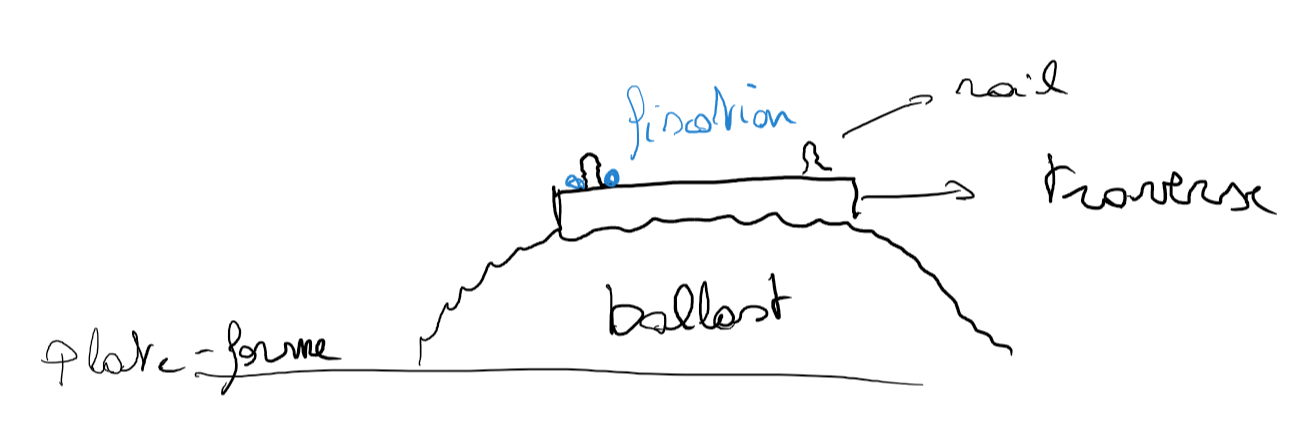
\includegraphics{infra_schema.PNG}
    \caption{Composants de la voie.}
    \label{infra_schema}
\end{figure}
\paragraph{Rail:}
Supporter la roue, guider la roue, répartir la charge sur les traverses. Leur surface de roulement doit être la plus lisse possible et leur géométrie est très importante dans le guidage des roues. Le rail doit supporter de très grandes forces (statiques et dynamiques) verticalement et latéralement. C'est pour cela qu'on utilise un alliage particulier.

\paragraph{Traverse:}
Supporter le rail, maintenir l'écartement, assurer la position de la voie, répartir la charge sur le ballast, garantir la position latérale de la voie.

\paragraph{Fixation du rail:}
 Fixer le rail, garantir l'écartement, isoler électriquement le rail, introduire de l'élasticité.
 
 \paragraph{Ballast:}
  Répartir la charge sur la plate-forme, garantir la stabilité de la traverse, évacuer les eaux de pluie, amortir les charges dynamiques, permettre l'adaptation et la correction de la géométrie de la voie.
  
  \paragraph{Plate-forme:}
  Garantir l'évacuation des eaux, relevage des courbes, ... .
  
  Tous les éléments ci-dessus ont comme fonction de soutenir les essieux d'un train et de répartir progressivement les efforts (Figure \ref{track_pressure}).
  \begin{figure}[H]
      \centering
      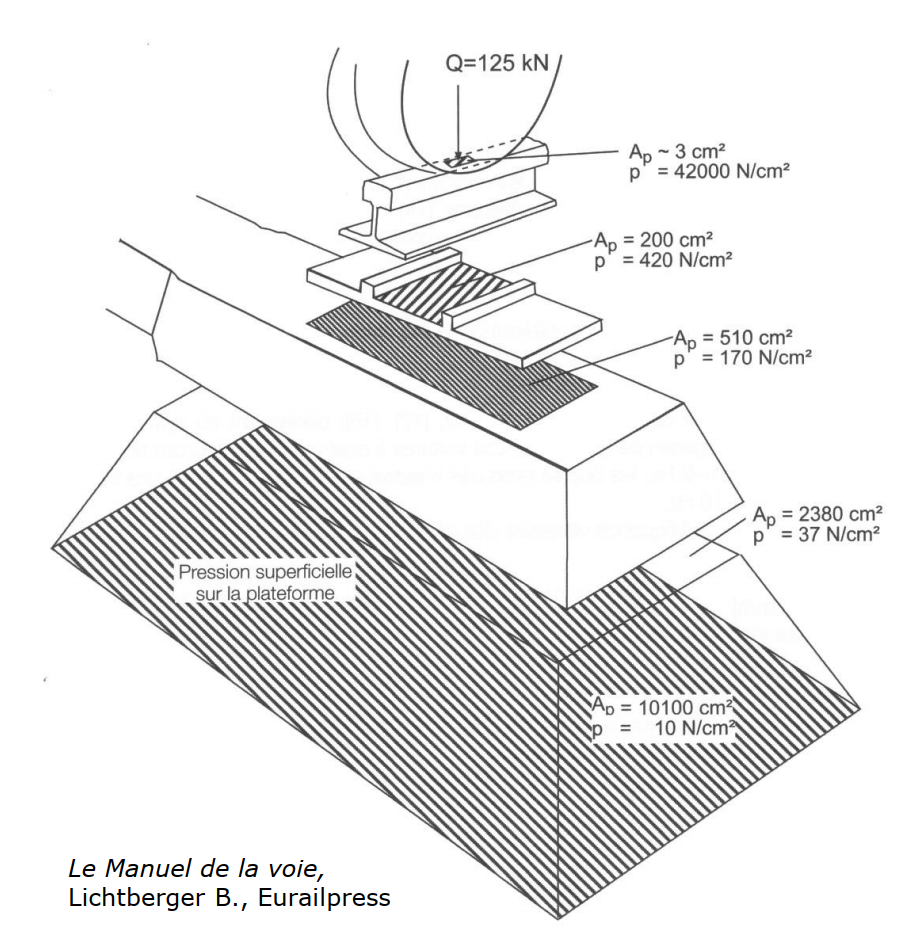
\includegraphics{track_pressure.PNG}
      \caption{Répartition de la pression due au passage d'un train sur les différents étages de la voie.}
      \label{track_pressure}
  \end{figure}
  
  \paragraph{Appareil de voie :}
  Nom donné aux aiguillages.
  
  \paragraph{Courbures :}
  Exemple de rayon de courbure minimal:
  \begin{itemize}
      \item 190 m pour des trains classiques
      \item 60 - 90 m pour des voie industrielles (usines, ...)
      \item 30 - 60 m pour les réseaux de métro
      \item 20 - 30 m pour les réseaux de tramways
  \end{itemize}
  
 Tout cela parce que un bogie classique n'a pas de mécanisme de direction!
 
 \paragraph{Dévers $h_t$ et angle de dévers $\phi_t$:}
Le dévers (Figure \ref{devers}) est utilisé pour compenser l'effet centrifuge en courbe. Les valeurs maximales de celui-ci sont généralement autour de $15 \ cm$ voire ($18$ ou même $20 \ cm$ pour les ligne uniquement passager). Cette compensation est utile pour réduire les efforts latéraux dans les rails, mais aussi pour augmenter le confort des passagers !
\begin{figure}[H]
    \centering
    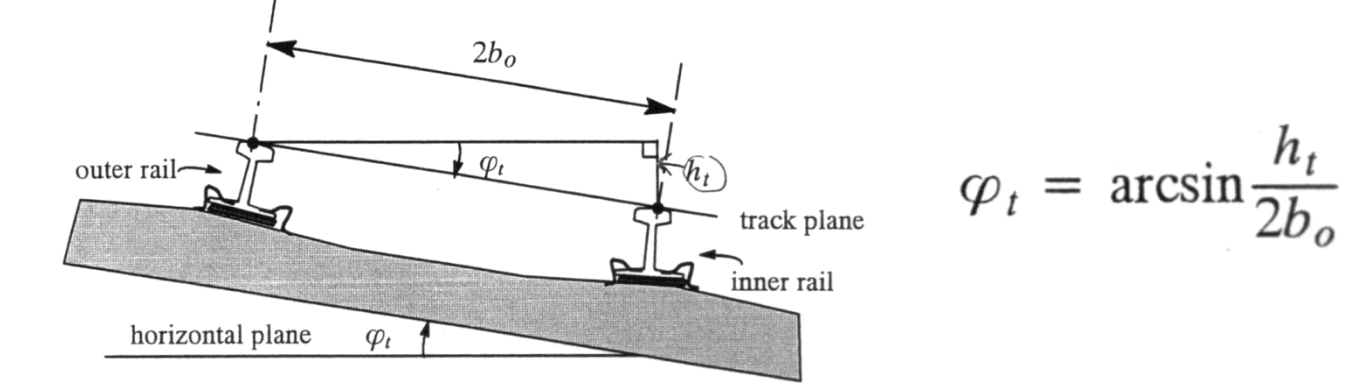
\includegraphics{devers.PNG}
    \caption{Dévers et angle de dévers.}
    \label{devers}
\end{figure}

\paragraph{Défauts de voie:}
En plus des défauts de rail possibles (irrégularités, défauts locaux), la voie complète peut avoir des défauts comme illustré sur la Figure \ref{track_pressure}. 
\begin{figure}[H]
    \centering
    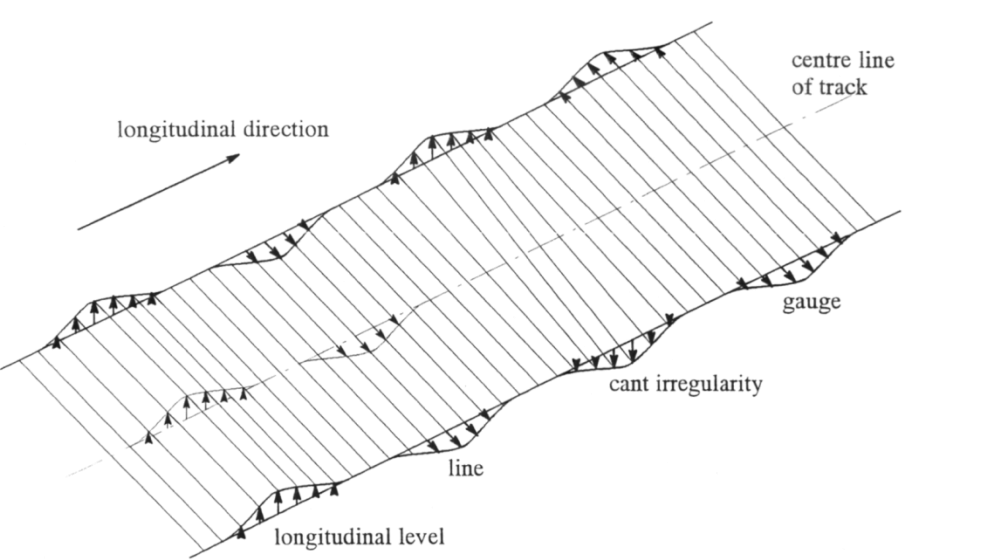
\includegraphics{default_track.PNG}
    \caption{Irrégularités de la voie}
    \label{default_track}
\end{figure}
Ces défauts peuvent être mesurés grâce à des trains spéciaux et étudiés en domaine temporel ou fréquentiel.

\paragraph{Flexibilité de la voie:}
La voie a une flexibilité verticale qui varient en fonction de nombreux paramètres (comme le moment dans l'année, le fait qu'il gèle ou pas, ...). Les traverses en bois sont plus flexibles que celles en béton. La déformation du rail entre les traverses est très faible, mais provoque tout de même des vibrations (qui sont beaucoup étudiées en recherche).
La flexibilité latérale est aussi importante pour les modèles dynamiques, même si celle-ci est assez peu étudiée !
On peut modéliser le rail comme posé sur un ressort amortisseur dont les raideurs/amortissement dépendent de la position en x (typiquement si on est sur ou entre des traverses) et un ressort amortisseur latéral constant complète le modèle.

\subsection{Critères de sécurité :}
En ferroviaire on s'intéresse généralement à deux forces: la force latérale $Y$ et la force verticale $Q$.
\begin{figure}[H]
    \centering
    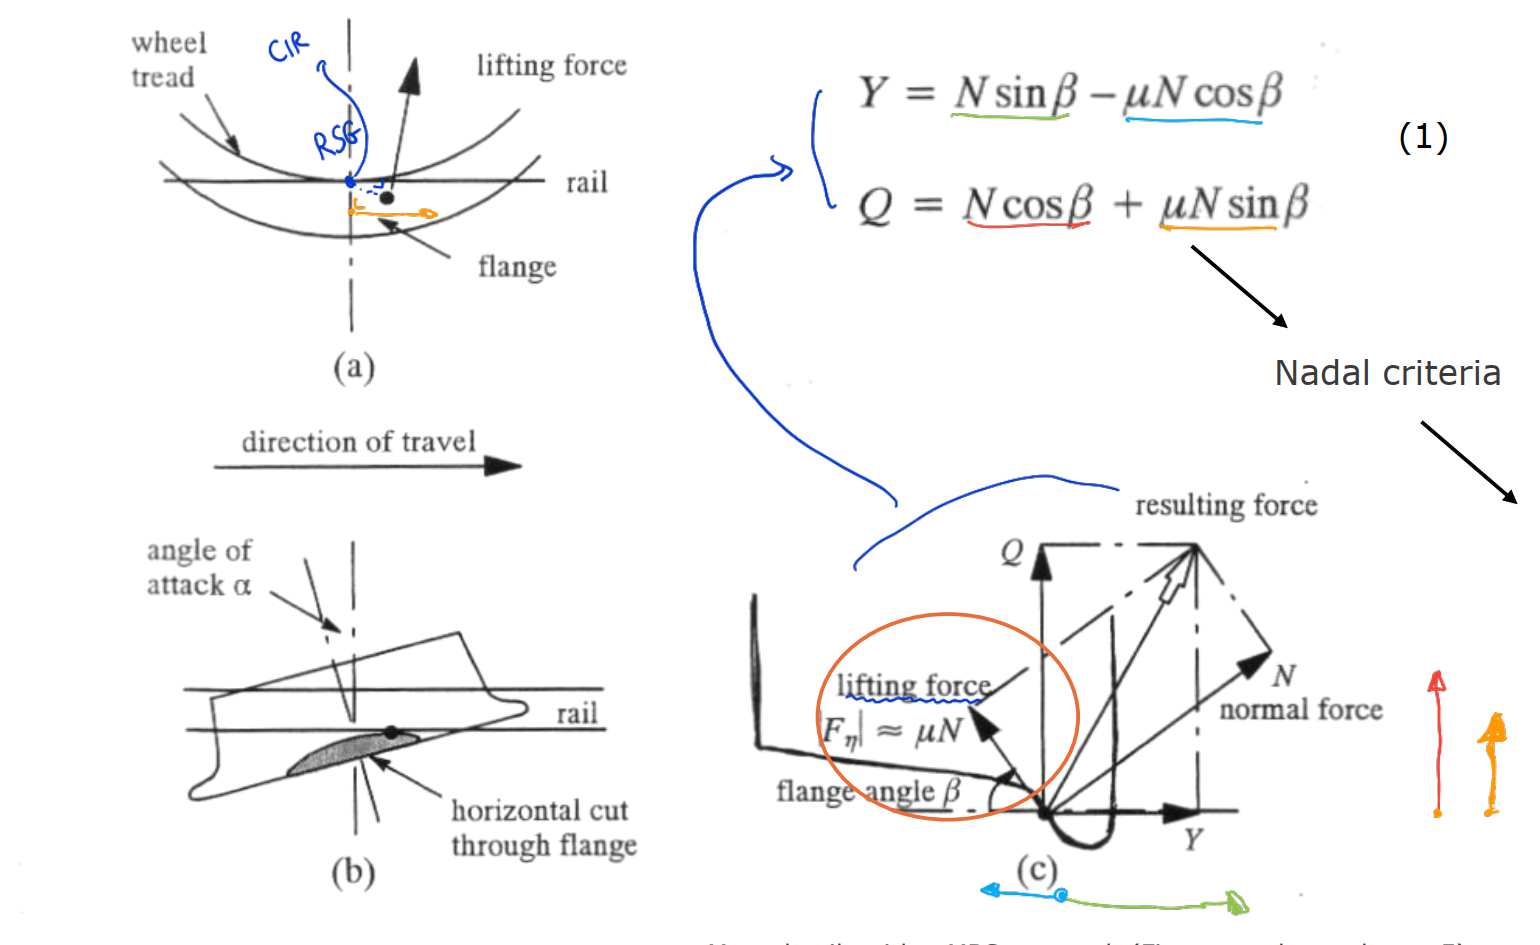
\includegraphics[width =0.8 \textwidth]{nadal1.PNG}
\end{figure}
\begin{figure}[H]
    \centering
    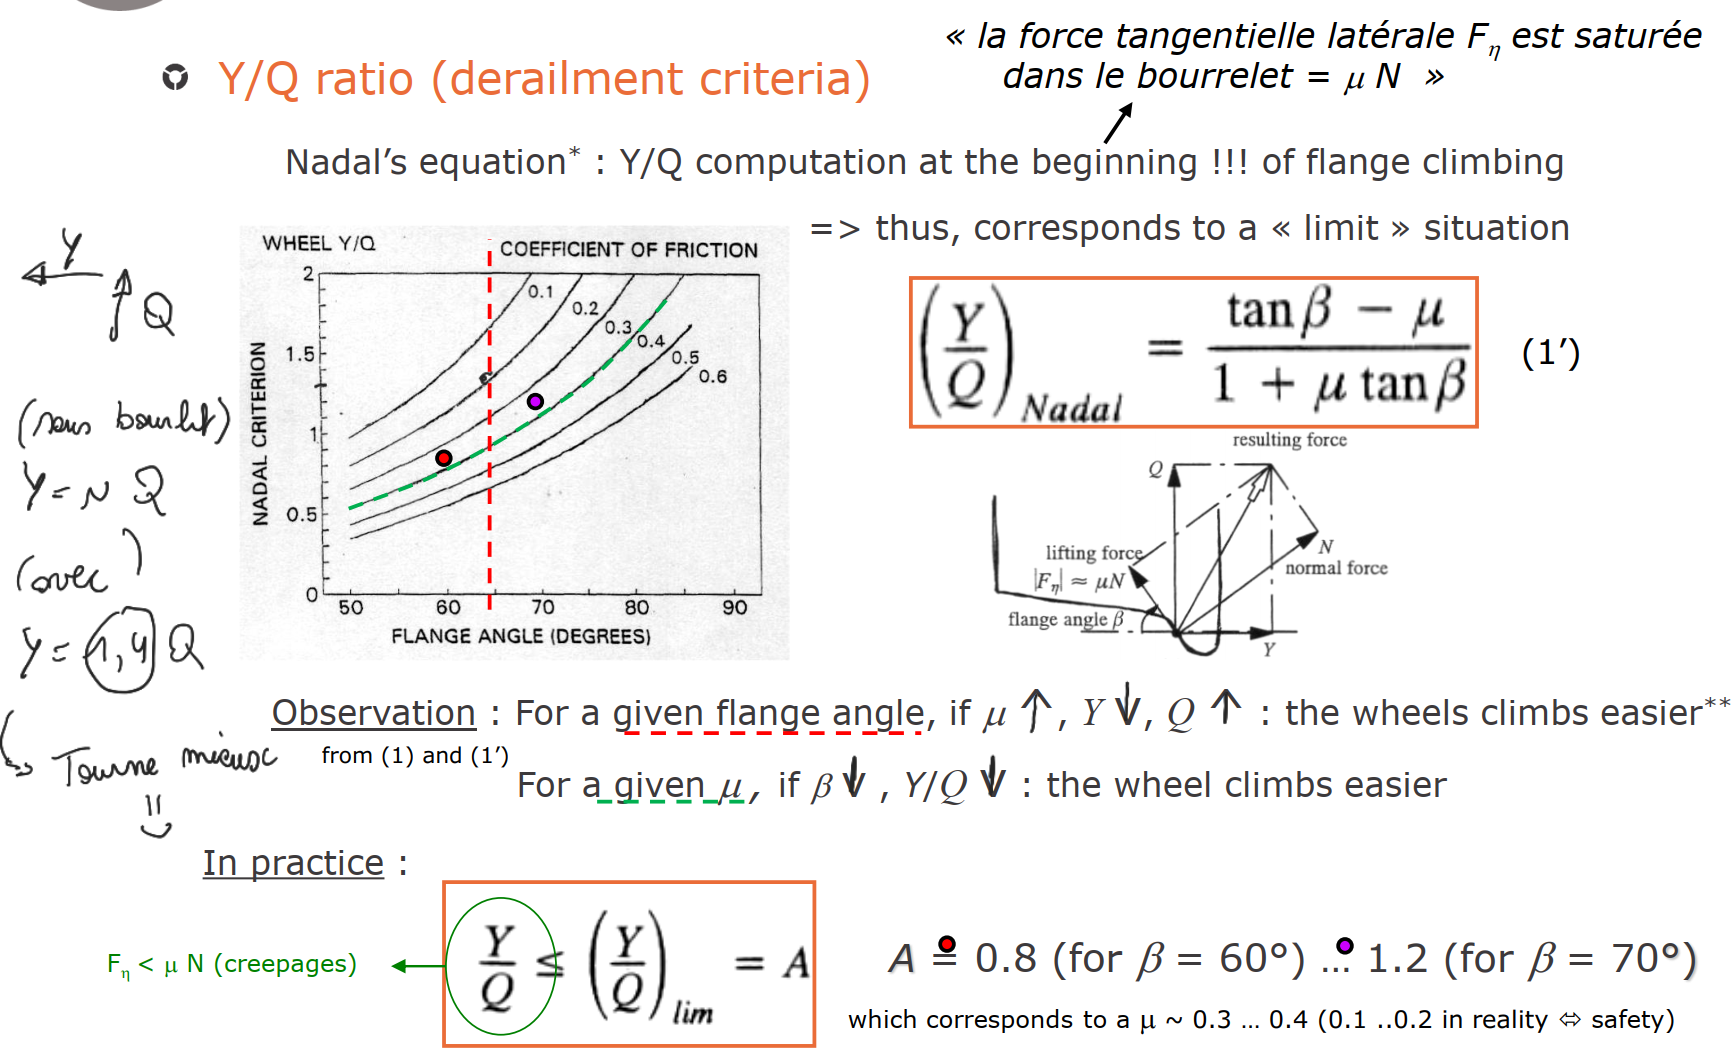
\includegraphics[width =0.8 \textwidth]{nadal2.PNG}
\end{figure}

On remarque que le $\cfrac{Y}{Q}$ diminue lorsque le coefficient de frottement augmente... c'est parce que le boudin accorche mieux au rail et monte dessus $\rightarrow$ grand Q! (Note: $\beta$ est l'angle que forme le boudin avec la surface de roulement). 

\begin{figure}[H]
    \centering
    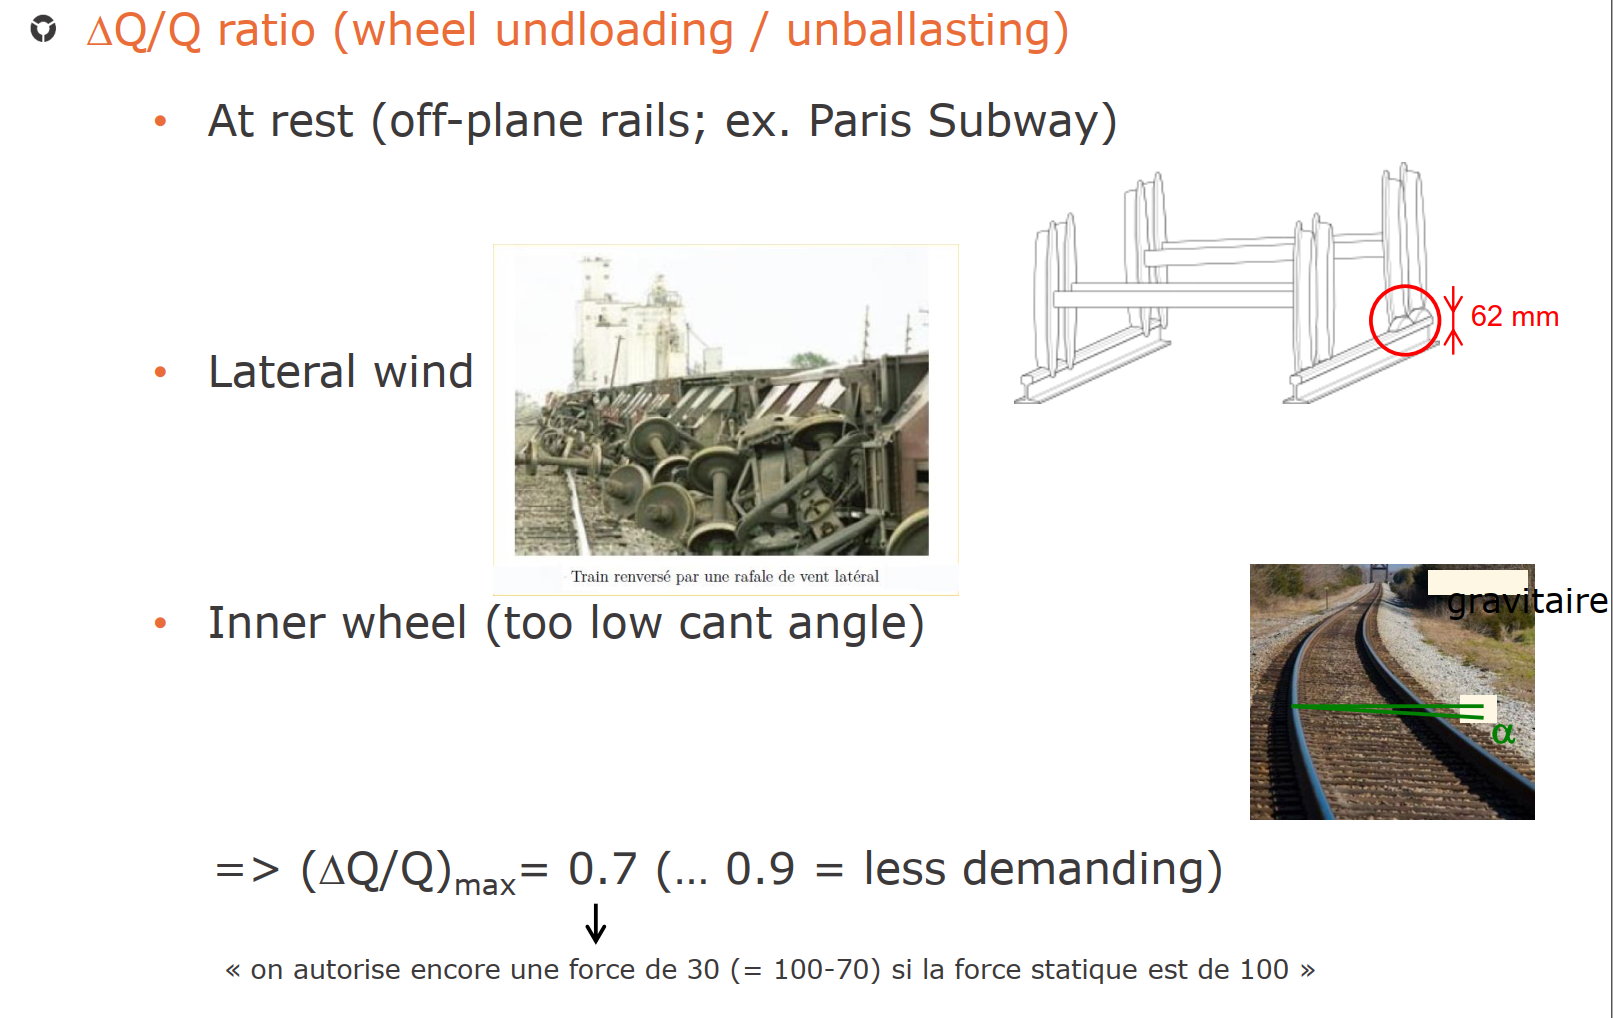
\includegraphics[width =0.8 \textwidth]{unballasting.PNG}
\end{figure}

Pour ce qui est du confort, tout est normé est les normes se basent essentiellement sur des valeurs RMS autour de certaines fréquences. Le niveau de la norme dépend du temps passé dans le véhicule (un tram peut être moins confortable qu'un TGV).

\section{Contact ferroviaire :}
La norme actuelle est pour des rail UIC60 combinés à des roues S1002.
Le calcul des points de contact entre les deux est un problème géométrique complexe, d'autant plus que lorsque les roues/rails sont neuf, ils présentent des points de contact discontinus $\rightarrow$ "jump" de points de contact.
Pour les tramways, le problème est légèrement différent puisqu'on a fréquement un double point de contact: un point au niveau de la bande de roulement qui reste tout le temps présent, et un point intermittent sur le boudin $\rightarrow$ contanct "Bang-Bang".

\subsection{Modèle cinématique simplifié}
On considère l'essieu comme un bi-cone. Les vitesses des centres des roues sont données par ($\delta_0$ est la conicité, $\omega$ la vitesse angulaire de l'essieu, $\psi$ l'angle de lacet de l'essieu, $2 l_0$ la voie):

\begin{minipage}{0.65 \textwidth}
    \begin{figure}[H]
        \centering
        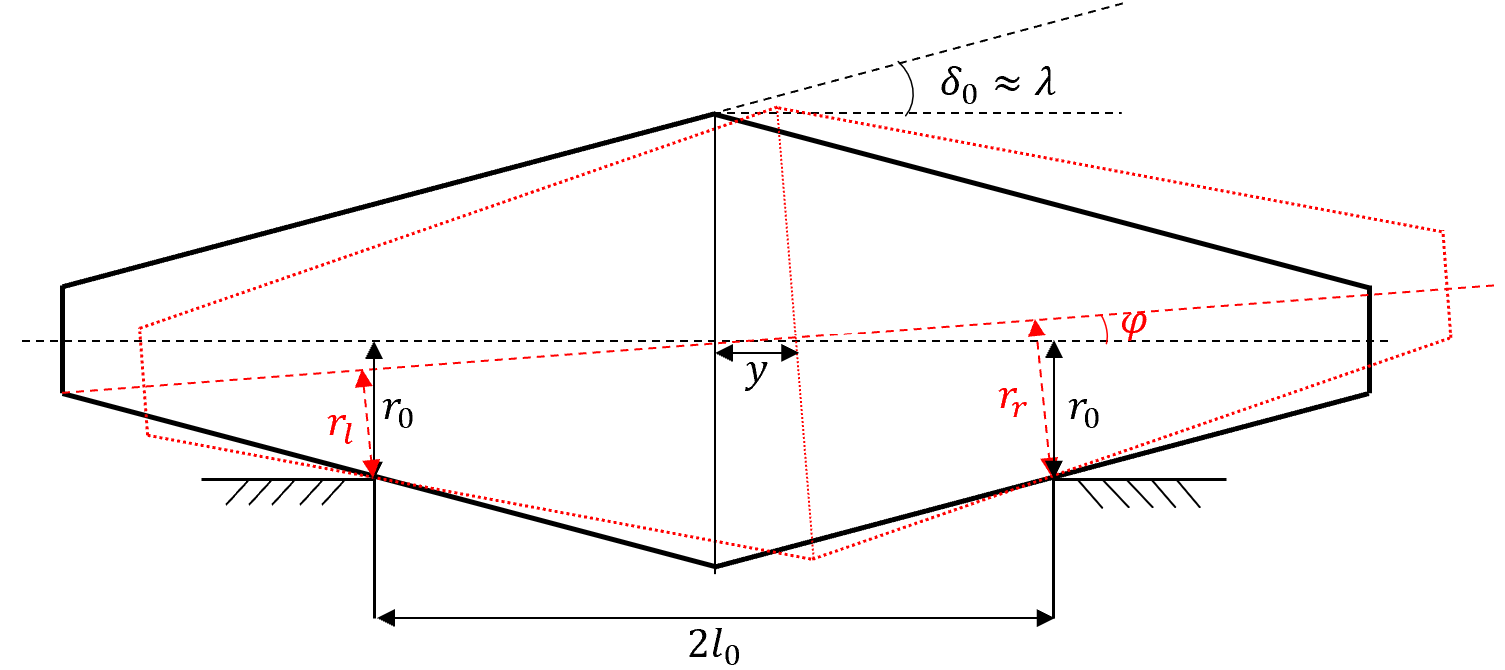
\includegraphics[scale=0.6]{cone_wheelset.png}
    \end{figure}
\end{minipage}
\hspace{1.7cm}
\begin{minipage}{0.3 \textwidth}
    \begin{align*}
        V_l &= \omega r_l \\
        V_r &= \omega r_r\\
        \lambda &= \tan{\delta_0}
    \end{align*}
\end{minipage}

Où les rayons $r_r$ et $r_l$ dépendent du déplacement latéral et de la conicité, on peut trouver leur valeur par approximation linéaire. En effet, si la conicité et petite. On peut représenter la situation de la manière suivante :

\begin{minipage}{0.45 \textwidth}
    \begin{figure}[H]
        \centering
        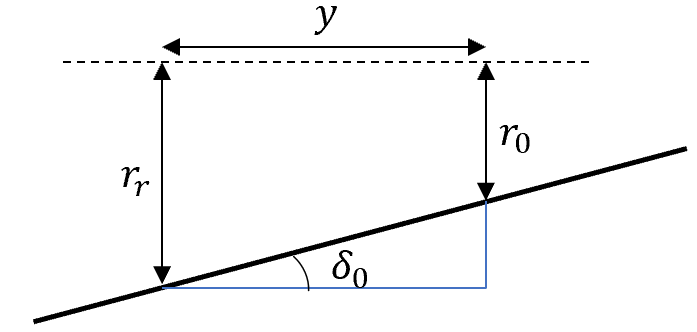
\includegraphics[scale=1]{cone_rayon.png}
    \end{figure}
\end{minipage}
\begin{minipage}{0.45 \textwidth}
    \begin{align*}
        \lambda &= \tan{\delta_0} \simeq \delta_0\\
        r_l &= r_0 - y \lambda \simeq r_0 - \delta_0 y\\
        r_r &= r_0 + y \lambda \simeq r_0 + \delta_0 y
    \end{align*}
\end{minipage}

Tandis que la vitesse de l'essieu est la moyenne des vitesses précédentes:
$$V = \cfrac{V_l + V_r}{2} = \omega r_0$$
Il est clair que si l'essieu a subit un (petit) dé-centrage latéral $y$ et un (petit) angle de lacet $\psi$, alors comme on l'a vu précédemment les rayons droite/gauche seront différent. Cela entraînera une différence de vitesse linéaire entre la partie droite et gauche de l'essieu entraînant une vitesse en lacet. 

De plus, la présence d'un angle de lacet entraîne une composante latérale de la vitesse du centre de l'essieu: 
\begin{align*}
    \overset{.}{y} &= V sin \psi \approx V \mathbf{\psi} \\
    \overset{.}{\psi} &= \cfrac{V_l - V_r}{2 l_0} = - \cfrac{\omega \Delta r}{2 l_0} = - \cfrac{V}{l_0 r_0} \lambda \mathbf{y}
\end{align*}
Ce modèle simplifié ne permet pas de prédire la stabilité car il s'agit bien d'un modèle cinétique, mais permet déjà de déterminer la fréquence de lacet de l'essieu (équations différentielles donc solution périodique) :
$$ f = \cfrac{V}{2 \pi} \sqrt{\cfrac{\lambda}{l_0 r_0}}$$

\subsection{Creepages}
Le terme creepage définit le contact de 2 matériaux lorsqu'ils ne sont ni tout à fait glissement pure l'un par rapport à l'autre ni en non-glissement. 
\paragraph{\textbf{Théorie de Hertz} :} 
Selon la théorie de Hertz, 2 corps élastique en contact forme une zone de contact elliptique dans laquelle, la pression est répartie suivant un champs parabolique. 

\begin{minipage}{0.45 \textwidth}
    \begin{figure}[H]
        \centering
        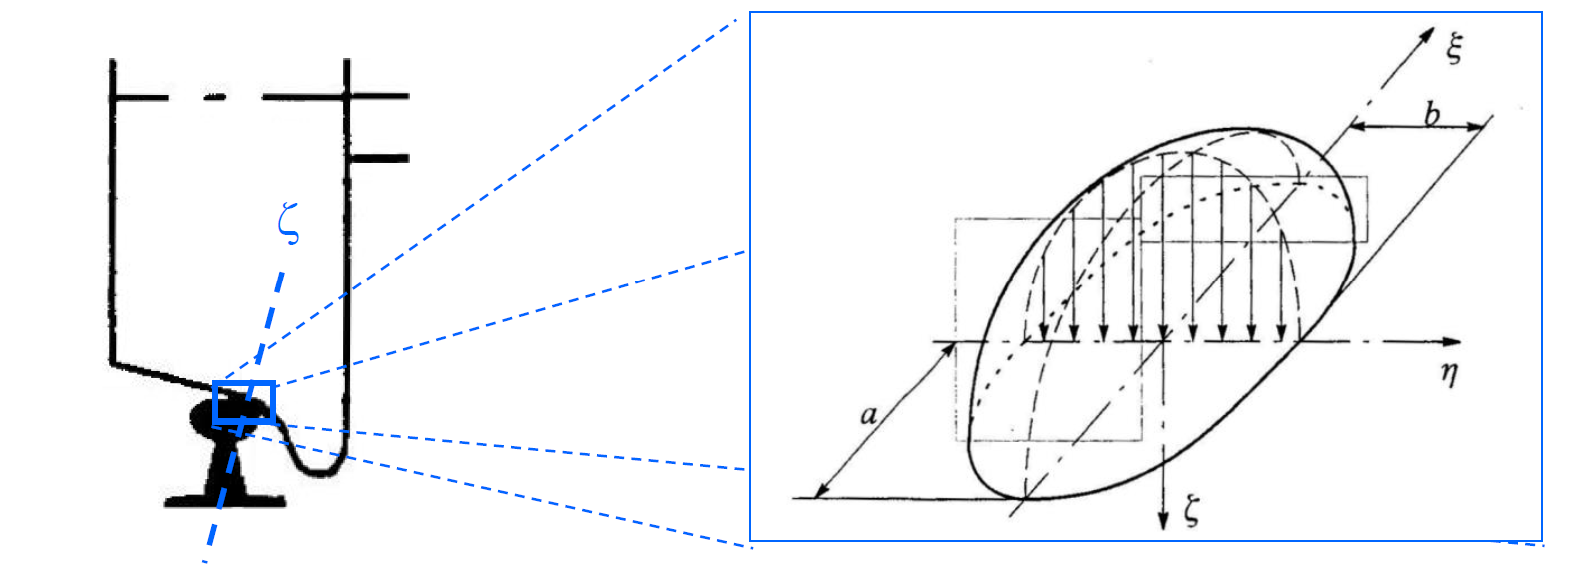
\includegraphics[scale=0.6]{Hertz.png}
    \end{figure}
\end{minipage}
\hspace{1.7cm}
\begin{minipage}{0.45 \textwidth}
    \begin{equation*}
        p(x,y) = \frac{3}{2}\frac{P}{2\pi ab} \sqrt[3]{1-\frac{x^2}{a^2}-\frac{y^2}{b^2}}
    \end{equation*}
\end{minipage}
    
\paragraph{\textbf{Théorie de Carter (1926)} :} 
Cette théorie introduit la notion de creepage : l'ellipse de contact à une partie d'adhésion et l'autre de glissement créant donc un "creep" longitudinal.

\begin{minipage}{0.45 \textwidth}
    \begin{figure}[H]
        \centering
        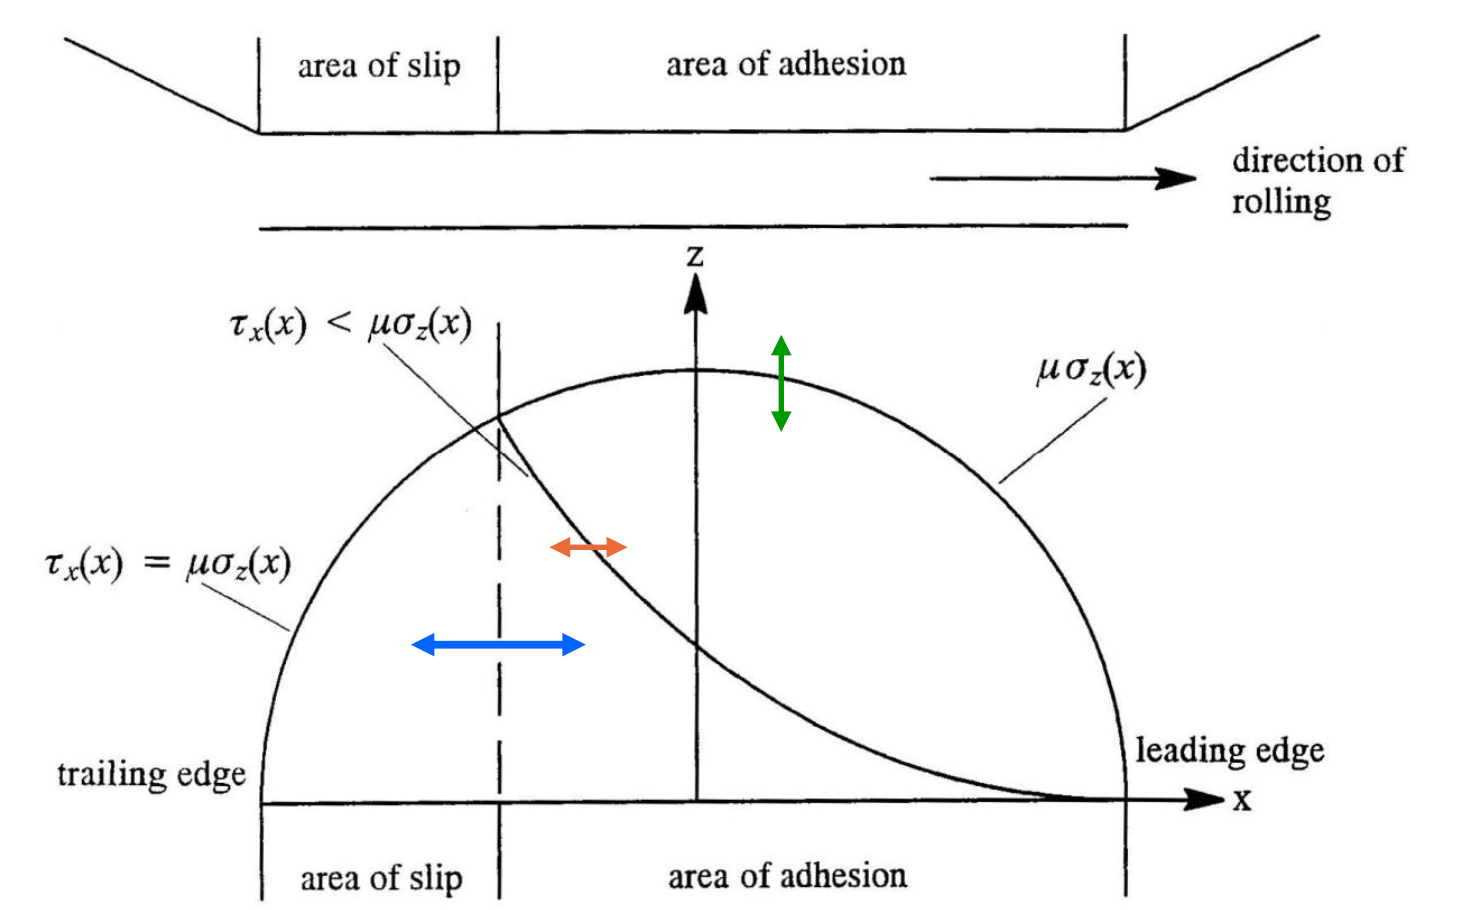
\includegraphics[scale=0.5]{brush.png}
    \end{figure}
\end{minipage}
\hspace{1.7cm}
\begin{minipage}{0.45 \textwidth}
    Explication via le modèle du pinceau, quand un poil entre dans la zone de contact, il commence à se déformer créant donc une contrainte $\tau(x)$. Ce poil va se déformer jusqu'au moment où $\tau(x)$ atteint la limite de friction $\mu \sigma_z(x)$, à partir de cet instant, le poil se met à glisser.
\end{minipage}

\paragraph{\textbf{Théorie de Johnson et Vermeulen (1958)} :} 
Elle étend la théorie précédente et permet le calcul des creepage longitudinaux et latéraux. Donc toujours pas de spin + mène à des erreurs de plus de 25\% par rapport aux résultats expérimentaux

\paragraph{\textbf{Théorie de Kalker (1967)} :}
En 1967 Kalker donne une étude exhaustive des différents cas de contact possibles entre deux sphères élastiques ayant un contact qui n'est pas un pur roulement sans glissement.
\begin{figure}[H]
    \centering
    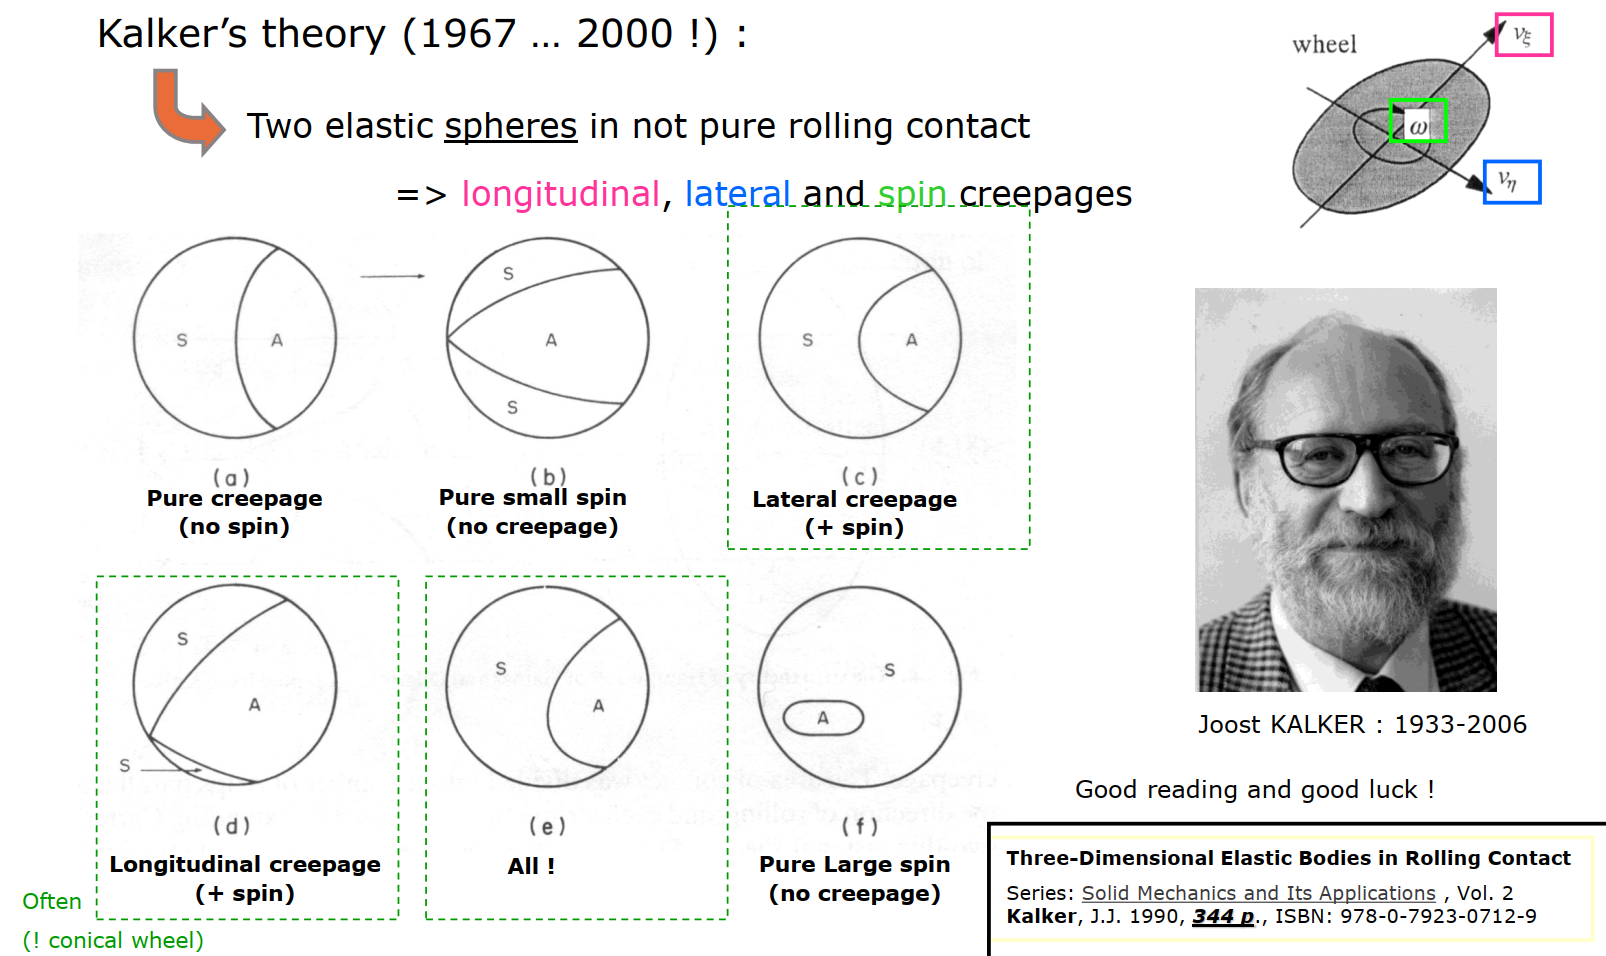
\includegraphics[width = 0.8\textwidth]{kalker1.PNG}
\end{figure}

Les creepages sont calculés par les expressions suivantes:
\begin{align}
\label{creepages}
    \gamma_{\epsilon} &= \cfrac{v_{\epsilon}}{v} \ [.]\\
    \gamma_{\eta} &= \cfrac{v_{\eta}}{v}  \ [.]\\
    \phi_{\zeta} &= \cfrac{\omega_{\zeta}}{v}  \ [1/m]
\end{align}
Où $v$ est la vitesse du centre de la roue et les directions sont prises par rapport au plan de contact. Les différentes vitesses prises au niveaux du contact peuvent être évaluées sur base de quelques hypothèses\footnote{ATTENTION : Ici, les $v_{\xi,l}$, $v_{\eta,l}$ et $\phi_{l}$ sont bien les creepages comme définit ci-avant et pas les vitesses matérielles du point de contact}:
\begin{figure}[H]
    \centering
    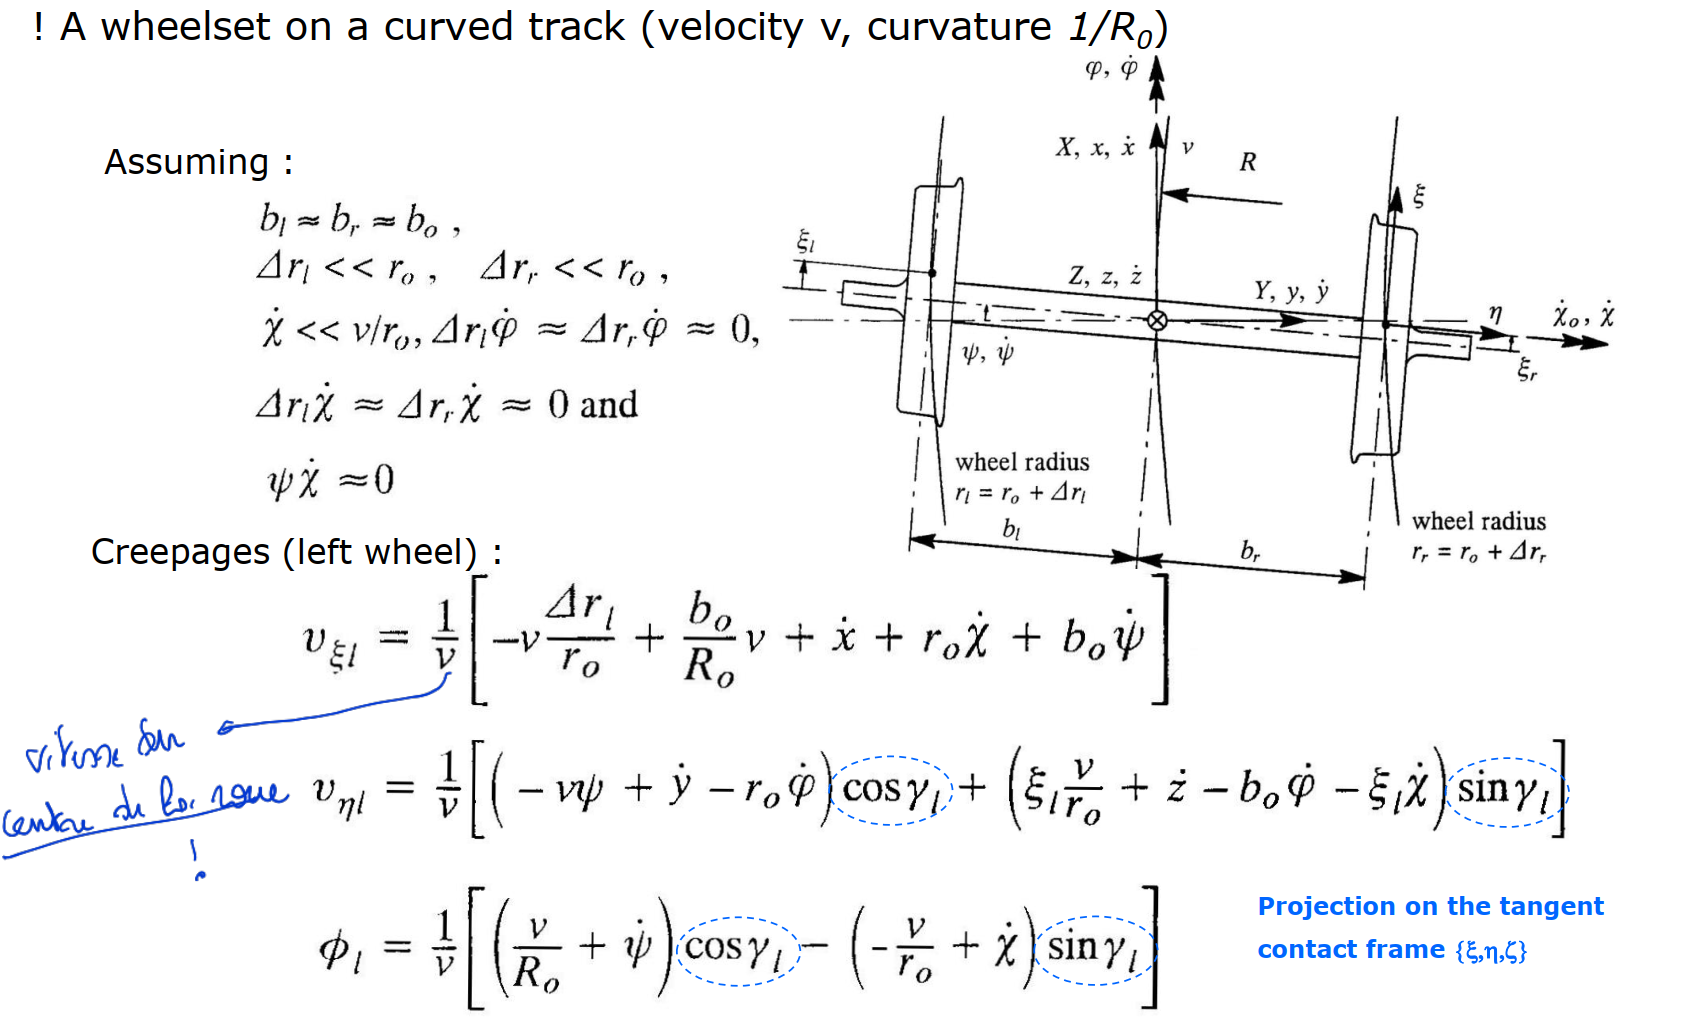
\includegraphics[width = 0.8\textwidth]{kalker2.PNG}
\end{figure}

Remarquons un point très important, les creepages sont définit par \textbf{rapport à la vitesse du centre de l'essieu}. La raison n'est pas d'adimentionnaliser ces grandeur à partir du moment ou cela ne marche pas pour le creepage angulaire $\phi_{\zeta}$ ($rad/s \cdot 1/(m/s)$). En effet, comme nous l'avons vu, les forces de contact sont dues aux déformations (en $mm$) et pas directement du glissement (en $mm/s$). Ainsi, avoir 2 fois plus de glissement en roulant deux fois plus vite reviens à la même chose (voir \autoref{2fois_plus_vite}). 
\begin{figure}[H]
    \centering
    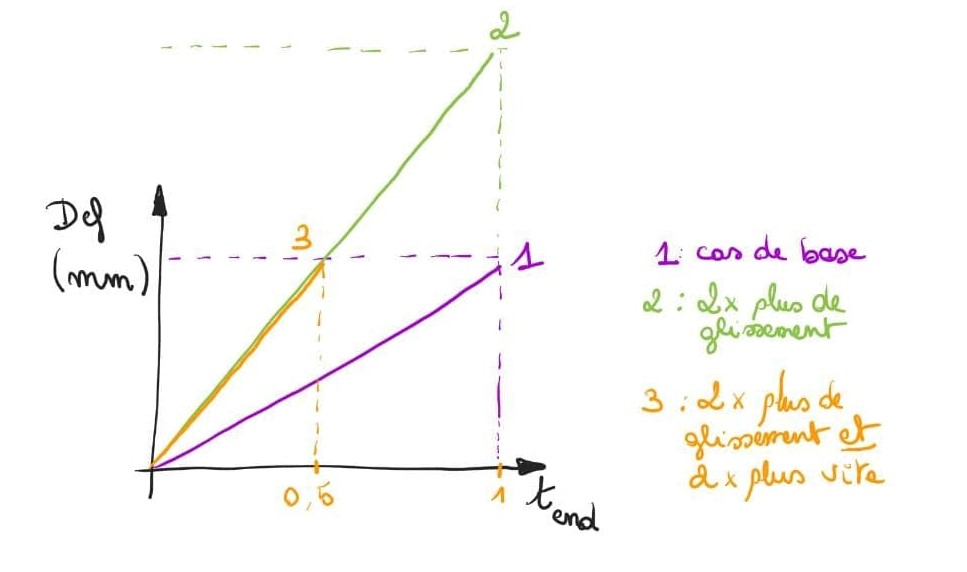
\includegraphics[width=0.7\textwidth]{2fois_plus_vite.jpg}
    \caption{2 fois plus de glissement 2 fois plus vite donne la même force longitudinale. Le contact dure deux fois moins longtemps et la déformation est donc identique.}
    \label{2fois_plus_vite}
\end{figure}

Pour obtenir les forces de contact (dues au creepages), la première étape est de partir de la théorie de Hertz::
\begin{align*}
    A &= \cfrac{1}{2} \Big ( \cfrac{1}{r_{\eta R}} - \cfrac{1}{r_{\eta}} \Big ) \\
    B &= \cfrac{1}{2} \Big ( \cfrac{1}{r_{\epsilon R}} - \cfrac{1}{r_{\epsilon}} \Big )  \\
    \theta &= arccos \Big(\cfrac{A-B}{A+B}\Big) \\
    a &= m \cdot \Big(\cfrac{3  \cdot (1 - \nu^2)\cdot F_N }{2 \cdot E \cdot (A+B)}\Big)^{1/3}\\
    b &= n \cdot \Big(\cfrac{3  \cdot (1 - \nu^2)\cdot F_N }{2 \cdot E \cdot (A+B)}\Big)^{1/3}
\end{align*}
Où $\nu$ est le coefficient de poisson du matériaux, $m$ et $n$ sont des coefficient de Herzt donnés par des tables (ou une interpolation de ces tables\footnote{Interpolation des tables de Hertz: \begin{align*}
    m &= 0.84 + 0.3981 \cdot 10^{-3} \cdot (4.05 - \theta)^{6.709}\\
    n &= 0.22 + 0.1383 \cdot (\theta + 0.88)^{1.845}
\end{align*}}) en fonction de l'angle $\theta$. 

Les coefficients de Kalker viennent eux de tables fonction de $m$ et $n$. \footnote{Un exemple d'interpolation est donné à titre illustratif (Berzeri Shabana and al., 2001):
\begin{align*}
    c_{11} &= 3.2893 + \cfrac{0.975 \cdot m}{n} - \cfrac{0.012 \cdot m^2}{n^2}\\
    c_{22} &= 2.4014 + \cfrac{1.3179 \cdot m}{n} - \cfrac{0.02 \cdot m^2}{n^2}\\
    c_{23} &= 0.4147 + \cfrac{1.0184 \cdot m}{n} + \cfrac{0.0565 \cdot m^2}{n^2} - \cfrac{0.0013 \cdot m^3}{n^3}\\
    c_{33} &= (0.16 + 0.3\frac{n}{m})\cdot 2 \cdot(1+0.3)\\
    \kappa_{11} &= G \cdot a \cdot b \cdot c_{11}\\
    \kappa_{22} &= G \cdot a \cdot b \cdot c_{22}\\
    \kappa_{33} &= G \cdot a^2 \cdot b^2 \cdot c_{33}\\
    \kappa_{23} &= G \cdot a \cdot b \cdot c_{23}\cdot \sqrt{a\cdot b}\\
    \kappa_{32} &= - \kappa_{23}\\
\end{align*}
Où $G$ est le module de cisaillement en $[N/m^2]$.}
Les force de roulements sont obtenue par les combinaisons linéaires suivantes :
\begin{align*}
    F_{\epsilon} &= - \kappa_{11} \cdot \gamma_{\epsilon} \\
    F_{\eta} &= - \kappa_{22} \cdot \gamma_{\eta} - \kappa_{23} \cdot \phi_{\zeta} \\
    M_{\zeta} &= - \kappa_{32} \cdot \gamma_{\eta} - \kappa_{33} \cdot \phi_{\zeta} 
\end{align*}

Pour approximer le comportement non-linéaire, une loi de saturation cubique peut être utilisée de sorte que la force totale de contact ne puisse dépasser $\mu \cdot F_N$. Pour se faire :

\begin{enumerate}
    \item On démarre de la loi linéaire de Kalker pour obtenir les forces de creepage
    \begin{eqnarray*}
        F'_{\xi} &=& - \kappa_{11} \cdot \gamma_{\epsilon} \\
        F'_{\eta} &=& - \kappa_{22} \cdot \gamma_{\eta} - \kappa_{23} \cdot \phi_{\zeta} \\
    \end{eqnarray*}
    
    \item On obtient la force total de creepage comme somme vectorielle :
    \begin{equation*}
        F'_v = \sqrt{\left(F'_{\xi}\right)^2 + \left(F'_{\eta}\right)^2 }
    \end{equation*}
    \item On définit la variable k tel que :
    \begin{equation*}
        k \triangleq \frac{F'_v}{\mu N}
    \end{equation*}
    \item On définit la loi de saturation cubique pour obtenir la "vraie" force totale de creepage :
    \begin{equation*}
        F_v = \begin{cases} 
        \mu N \left(k-\frac{1}{3}k^2+\frac{1}{27}k^3\right), & \mbox{si } k \leq 3 \\ 
        \mu N, & \mbox{si } k \ge 3 
        \end{cases}
    \end{equation*}
    \item On obtient la "vraie" force longitudinale et latérale de creepage en supposant un respect des proportions entre ($F_v$, $F'_v$), ($F_{\xi}$, $F'_{\xi}$) et ($F_{\eta}$, $F'_{\eta}$)
    
    \begin{minipage}{0.45 \textwidth}
        \begin{figure}[H]
            \centering
            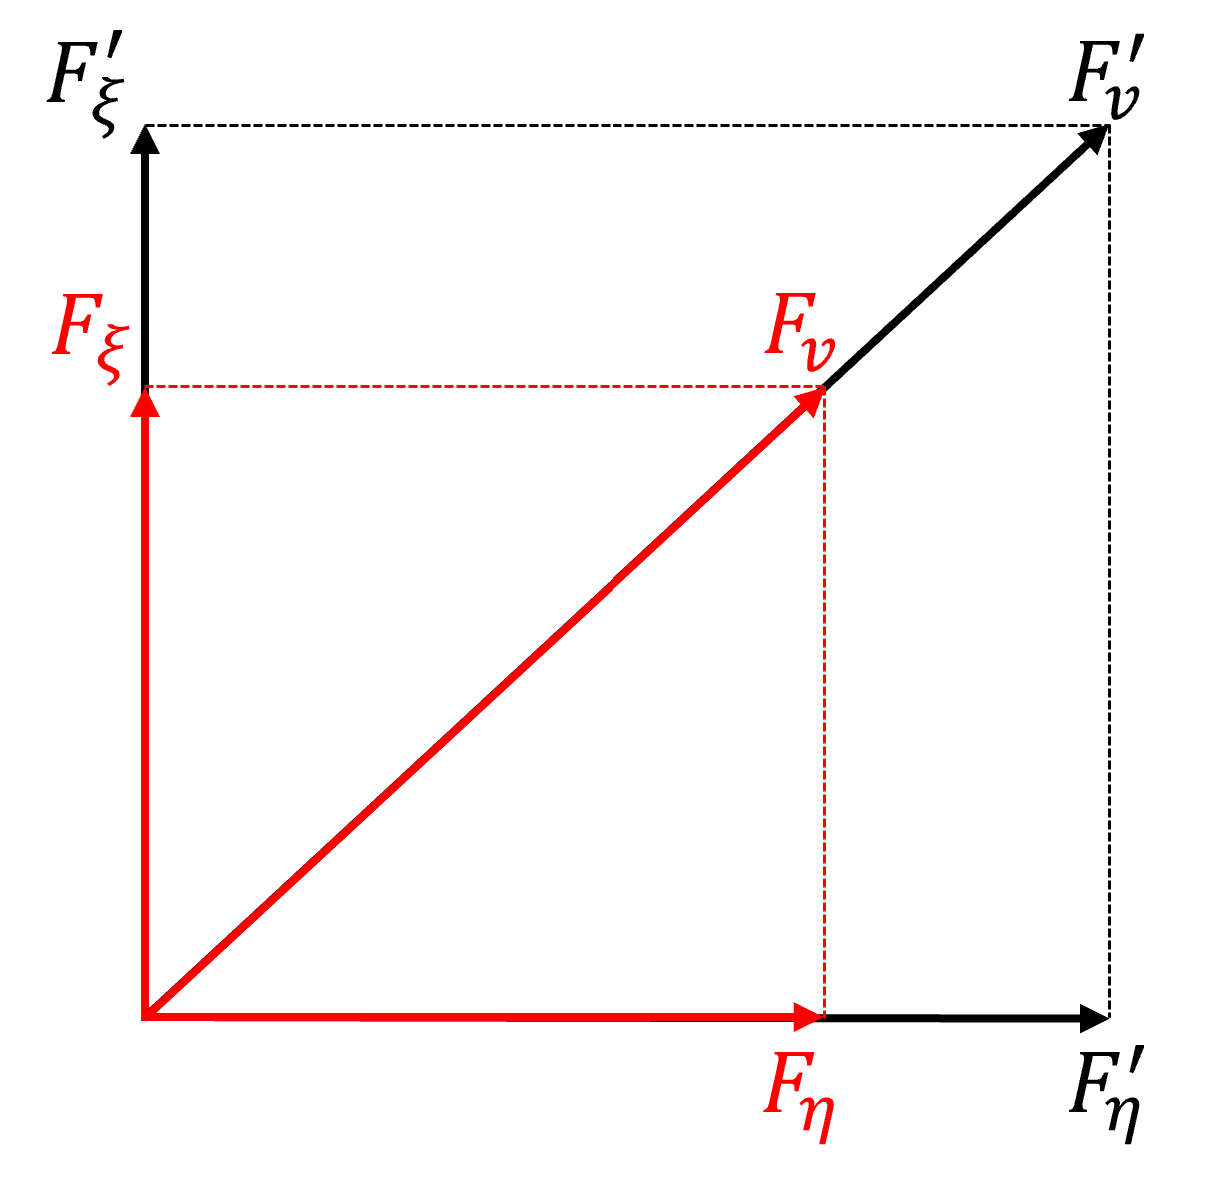
\includegraphics[scale=0.3]{Triangles_semblables.png}
        \end{figure}
    \end{minipage}
    \hspace{0.4cm}
    \begin{minipage}{0.45 \textwidth}
        Via le théorème de Thalès dans les triangles semblable rouge et noir, on a :
        \begin{equation*}
            \frac{F_{\eta}}{F'_{\eta}} = \frac{F_{\xi}}{F'_{\xi}} = \frac{F_{v}}{F'_{v}}
        \end{equation*}
    \end{minipage}
\end{enumerate}
On obtient donc l'expression des forces de creepages non-linéaires :
\begin{eqnarray*}
    F_{\xi} &=& \frac{F'_{\xi}}{F'_{v}} F_v \\
    F_{\eta} &=& \frac{F'_{\eta}}{F'_{v}} F_v \\
    M_{\phi} &=& - \kappa_{32} \cdot \gamma_{\eta} - \kappa_{33} \cdot \phi_{\zeta}
\end{eqnarray*}
Il faut bien remarquer qu'on a donc fait l'hypothèse de petit spin donc on n'a pas saturé le moment dû au creepage.

Une théorie de Kalker non-linéaire existe aussi ainsi que d'autre alternatives plus récentes !

\subsection{Essieu suspendu} 

\paragraph{\textbf{Dynamique linéaire :}}
Un train est un système dynamique très complexe. MAIS, 90\% de cette complexité provient du contact roue/rail. Donc, on peut analyser un essieu suspendu à vitesse constante sur un rail droit pour avoir une bonne idée de la dynamique générale du train.

\begin{figure}[H]
    \centering
    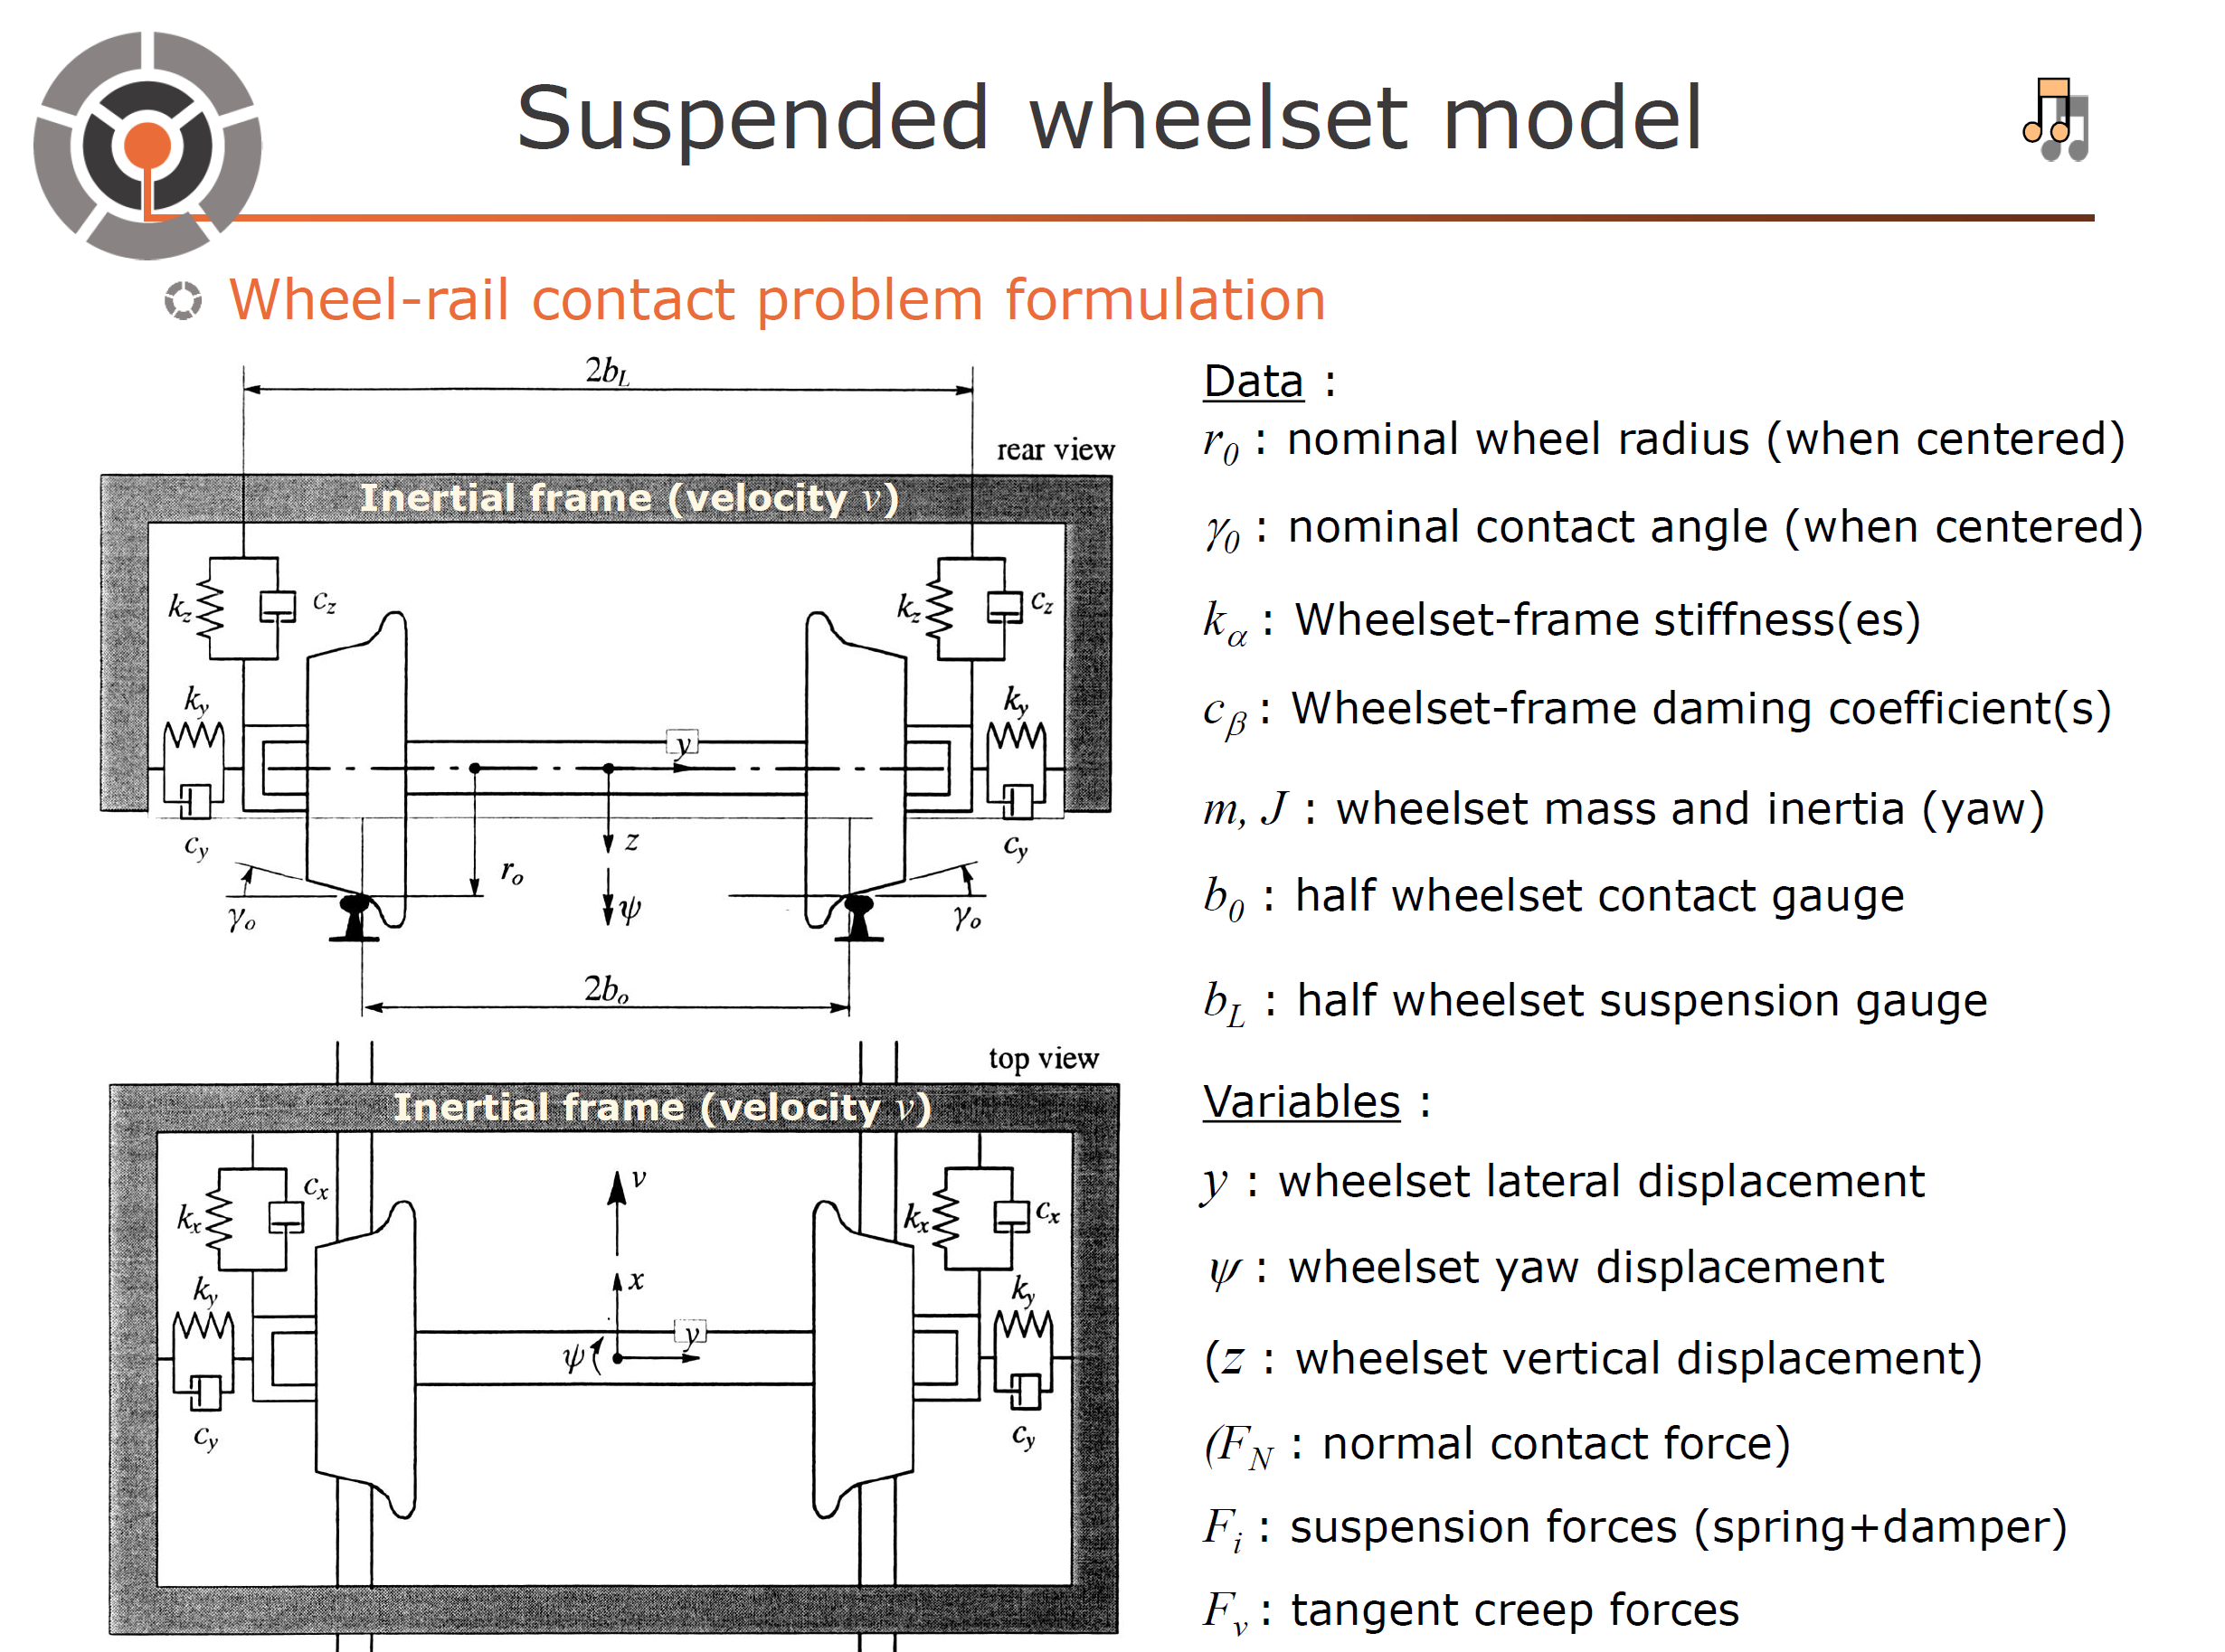
\includegraphics[width = 0.8\textwidth]{suspended_wheelset.png}
\end{figure}


Par ailleurs, nous prenons les hypothèses simplificatrices suivantes :
\begin{itemize}
    \item Le système n'a que 2 ddl en $y$ (mvt latéral) et $\psi$ (mvt de lacet)
    \item Linéarisation de toutes les quantités $(\cos{(\alpha)} = 1 \text{ et } \sin{(\alpha)} = \alpha)$
    \item Moment de spin négligé
    \item Force normale constante $(F_N = \frac{W}{2})$
\end{itemize}
Les équations du mouvement prennent donc la forme suivante : 
\begin{equation}
    \begin{bmatrix}
       m & 0 \\
       0 & J 
    \end{bmatrix} 
    \begin{bmatrix}
       \ddot{y} \\
       \ddot{\psi} 
    \end{bmatrix} 
    = 
    \begin{bmatrix}
       F_N 
    \end{bmatrix} +
    \begin{bmatrix}
       F_i 
    \end{bmatrix} +
    \begin{bmatrix}
       F_v
    \end{bmatrix} 
\end{equation}
Où 
\begin{itemize}
    \item $F_N = \begin{bmatrix} Y_N \\ 0 \end{bmatrix}$ décrit les forces normales de contact. Celles-ci n'induisent pas de couples car on les négliges,
    \begin{minipage}{0.45 \textwidth}
        \begin{figure}[H]
            \centering
            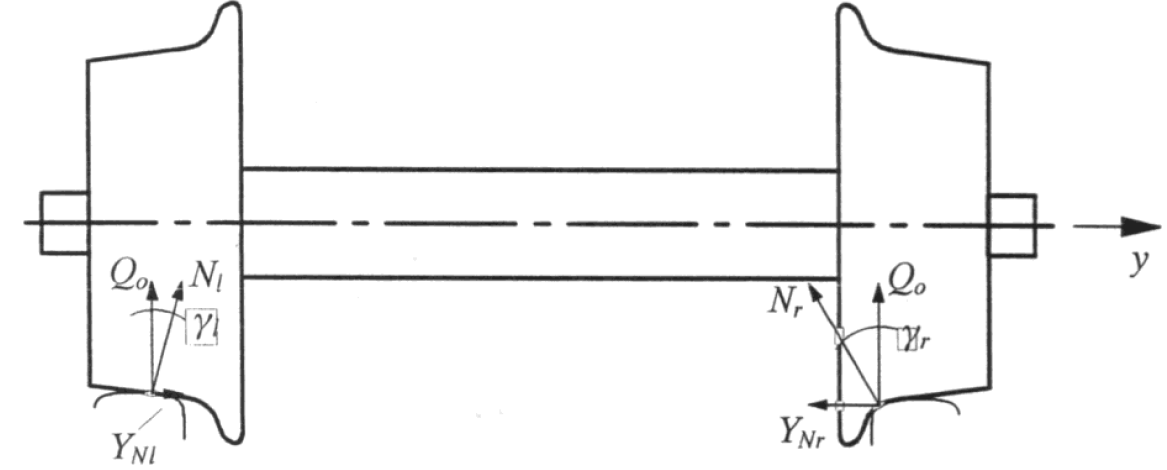
\includegraphics[scale=0.65]{grav_wheelset.png}
        \end{figure}
    \end{minipage}
    \hspace{1cm}
    \begin{minipage}{0.45 \textwidth}
        \begin{equation*}
            Y_N = -Q_0 (\tan{\gamma_r} - \tan{\gamma_l}) 
        \end{equation*}
    \end{minipage}
     On définit alors $\kappa = \frac{\tan{\gamma_r} - \tan{\gamma_l}}{2y}$, l'expression de la force peut alors s'écrire : 
        \begin{equation*}
            F_N = \begin{bmatrix} -2Q_0\kappa y  \\ 0 \end{bmatrix}
        \end{equation*}
    
     \item $F_i = \begin{bmatrix} F_{y,l} + F_{y,r} \\ M_{\psi}  \end{bmatrix}$ décrit les forces ressorts/amortisseurs, 
        
    \begin{minipage}{0.45 \textwidth}
        \begin{figure}[H]
            \centering
            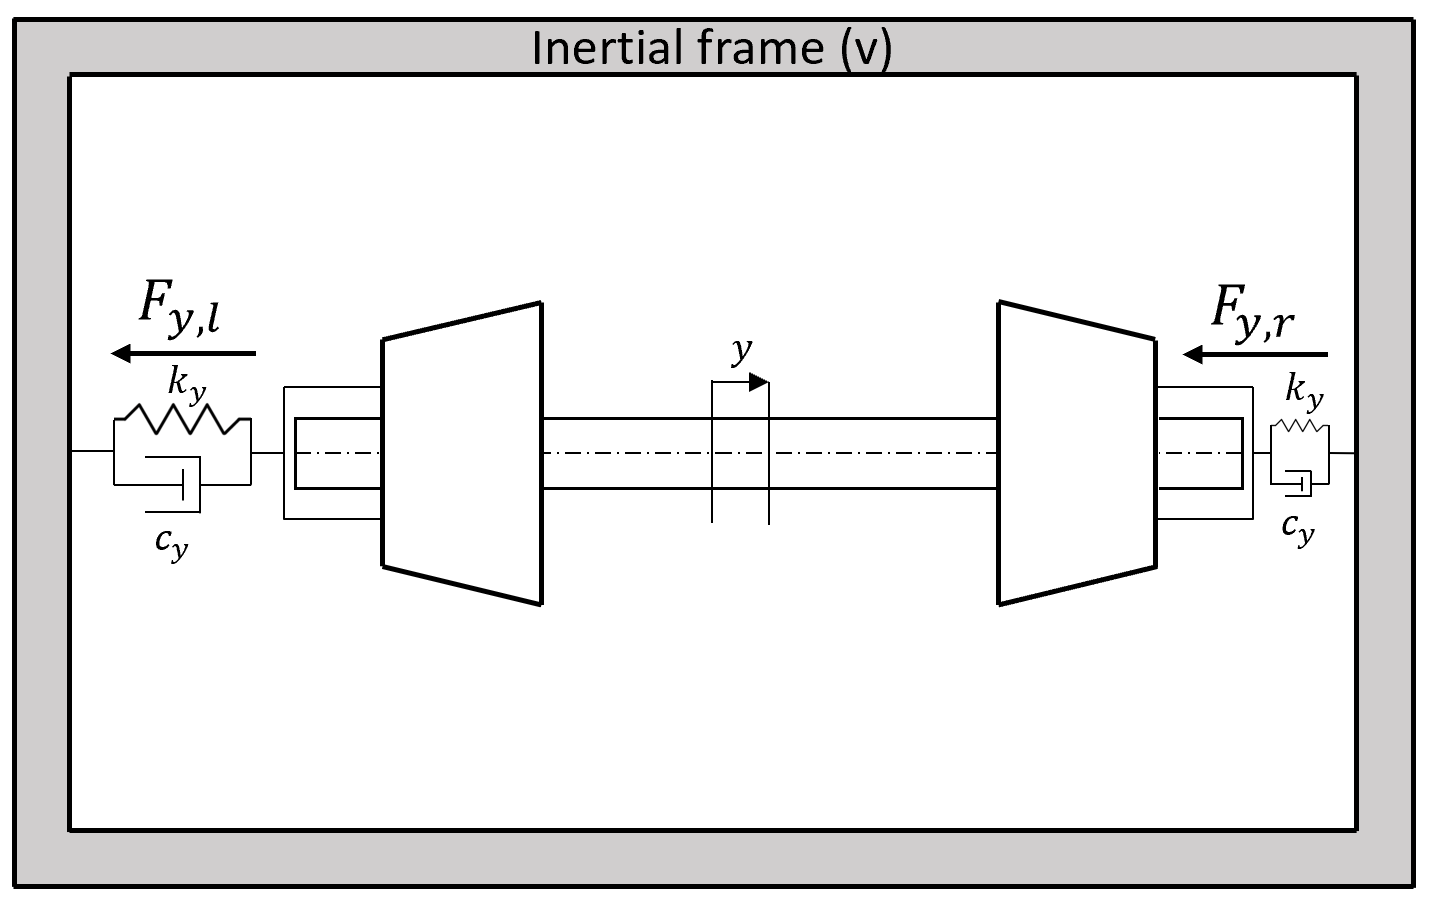
\includegraphics[scale=0.5]{Suspended_wheelset_lat.png}
        \end{figure}
    \end{minipage}
    \hspace{1cm}
    \begin{minipage}{0.45 \textwidth}
        \begin{eqnarray*}
            F_{y,l} &=& - \underbrace{\left( k_{y,l} \cdot y\right)}_{\text{Ressort}} - \underbrace{\left( c_{y,l} \cdot \dot{y}\right)}_{\text{Amortisseur}} \\
            F_{y,r} &=& - \underbrace{\left( k_{y,r} \cdot y\right)}_{\text{Ressort}} - \underbrace{\left( c_{y,r} \cdot \dot{y}\right)}_{\text{Amortisseur}} 
        \end{eqnarray*}
    \end{minipage}
    
    \begin{minipage}{0.45 \textwidth}
        \begin{figure}[H]
            \centering
            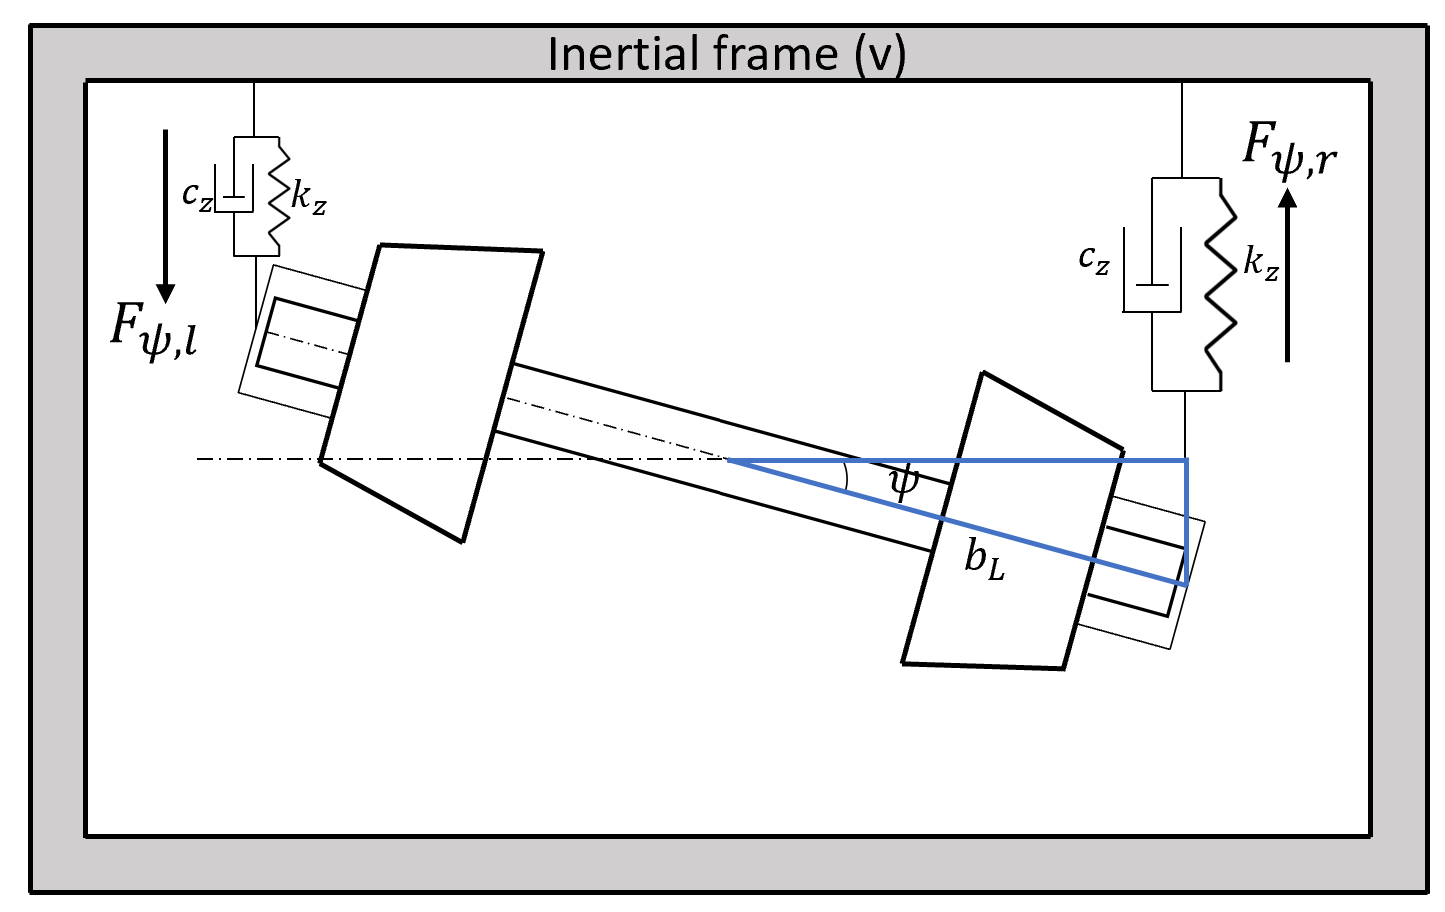
\includegraphics[scale=0.5]{Suspended_wheelset_lacet.png}
        \end{figure}
    \end{minipage}
    \hspace{1cm}
    \begin{minipage}{0.45 \textwidth}
        \begin{eqnarray*}
            M_{\psi} &=& b_L \left(F_{\psi,l} + F_{\psi,r}\right) \\
            &F_{\psi,l}& = - \underbrace{\left( k_{z,l} \cdot b_L \sin{\psi}\right)}_{\text{Ressort}} - \underbrace{\left( c_{z,l} \cdot b_L \dot{\psi}\right)}_{\text{Amortisseur}}\\
            &F_{\psi,r}& = - \underbrace{\left( k_{z,r} \cdot b_L \sin{\psi}\right)}_{\text{Ressort}} - \underbrace{\left( c_{z,r} \cdot b_L \dot{\psi}\right)}_{\text{Amortisseur}}
        \end{eqnarray*}
    \end{minipage}
    
    Étant donné que les coefficients de raideur et d'amortissement sont les mêmes à droite et à gauche, ainsi que par linéarisations ($\sin{\psi} = \psi$), les équations deviennent :
    
    \begin{equation*}
        F_i = \begin{bmatrix} -2\left(k_y\cdot y + c_y \cdot \dot{y}\right)  \\ -2b_L^2\left(k_x\cdot \psi + c_y \cdot \dot{\psi}\right)  \end{bmatrix}
    \end{equation*}
     
    \item $F_v = \begin{bmatrix} F_{v,y} \\ M_{v,\psi}  \end{bmatrix}$ décrit les forces tangentes de creepage, 
    
    \begin{minipage}{0.45 \textwidth}
        \begin{figure}[H]
            \centering
            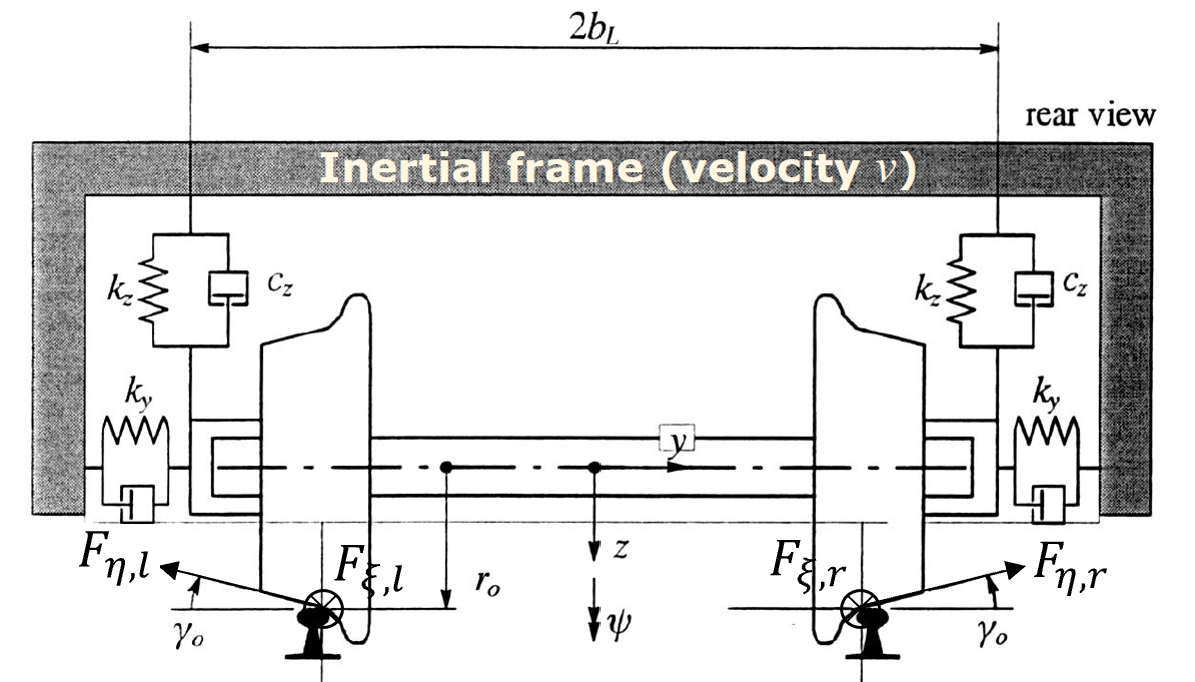
\includegraphics[scale=0.6]{Suspended_wheelset_creep.png}
        \end{figure}
    \end{minipage}
    \hspace{1cm}
    \begin{minipage}{0.45 \textwidth}
        \begin{eqnarray*}
            F_{v,y} &=&  \left(F_{\eta,l} + F_{\eta,r}\right) \cos{\gamma_0}\\
            M_{v,\psi} &=& \left(F_{\xi,l} - F_{\xi,r}\right) b_0
        \end{eqnarray*}
    \end{minipage}
    
    La force due aux creepages peut alors se réécrire :
    
    \begin{equation*}
        F_v = \begin{bmatrix} \left(F_{\eta,r} + F_{\eta,l}\right) \cos{\gamma_0} \\ -\left(F_{\xi,r} - F_{\xi,l}\right) b_0  \end{bmatrix}
    \end{equation*}
\end{itemize}
Ensuite, si on exprime les forces de creepages au moyen de la théorie linéaire de Kalker en se souvenant qu'il n'y a que 2 degrés de liberté, on peut obtenir le système suivant :

\begin{gather*}\renewcommand{\arraystretch}{2}
    \begin{bmatrix}
       m & 0 \\
       0 & J 
    \end{bmatrix} 
    \begin{bmatrix}
       \ddot{y} \\
       \ddot{\psi} 
    \end{bmatrix} 
    + 
    \begin{bmatrix}
       2c_y & 0 \\
       0 & 2b_L^2c_x 
    \end{bmatrix} 
    \begin{bmatrix}
       \dot{y} \\
       \dot{\psi} 
    \end{bmatrix} 
    + \frac{1}{v}
    \begin{bmatrix}
       2\kappa_{22} & 2\kappa_{23} \\
       0 & 2b_0^2\kappa_{11} 
    \end{bmatrix} 
    \begin{bmatrix}
       \dot{y} \\
       \dot{\psi} 
    \end{bmatrix} 
    + 
    \begin{bmatrix}
       2k_y + 2\kappa \left(Q_0 - \frac{\kappa_{23}}{r_0}\right) & -2\kappa_{22} \\
       \frac{2b_0\kappa_{11}\lambda}{r_0} & 2b_L^2k_x 
    \end{bmatrix} 
    \begin{bmatrix}
       y \\
       \psi
    \end{bmatrix} 
    =
    \begin{bmatrix}
       0 \\
       0
    \end{bmatrix} \\
    M \ddot{u} + C_i \dot{u} + \frac{1}{v} C_k \dot{u} + Ku = 0 
\end{gather*}

\textbf{Remarques : }
\begin{itemize}
    \item La matrice K est non-diagonale (c.à.d. couplage entre mouvement de lacet et mouvement latéral) et non-symétrique $\Rightarrow$ \textbf{Existence de solution(s) instable(s)},
    \item L'amortissement causé par les forces de "creep" (matrice $C_k$) est inversement proportionnel à la vitesse d'avance du train (c.à.d. Plus le train va vite, plus l'amortissement est faible) $\Rightarrow$ \textbf{Existence d'une vitesse critique pour l'essieu},
    \item Une grande partie de la raideur gravitationnelle ($2\kappa Q_0 y$) est neutralisée par le terme $2\kappa \frac{\kappa_{23}}{r_0}y$ et donc par les froces de "creep". Dès lors, la raideur gravitationnelle est souvent inefficace pour ramener le véhicule à sa position initiale $\Rightarrow$ \textbf{Pas beaucoup d'effet stabilisant pour les roues indépendantes (bogie 2000)}.
\end{itemize}

Le système dynamique étant linéaire, on peut analyser sa stabilité par l'étude des valeurs propres. Ce dernier a donc 4 valeurs propres (car système d'ordre 2), on peut voir que :

\begin{minipage}{0.45 \textwidth}
    \begin{figure}[H]
        \centering
        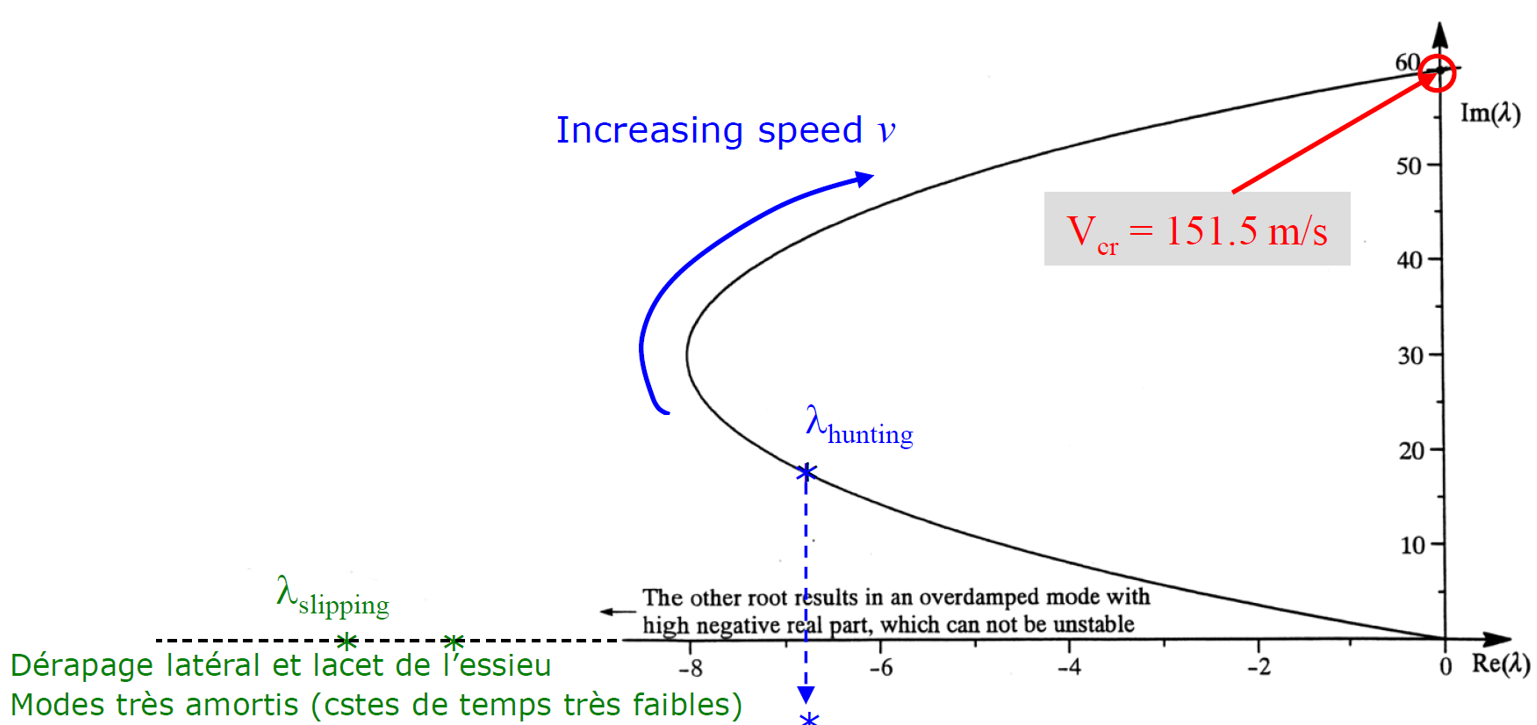
\includegraphics[scale=0.4]{root_locus.png}
    \end{figure}
\end{minipage}
\hspace{1cm}
\begin{minipage}{0.45 \textwidth}
    \begin{itemize}
        \item 2 d'entre elles sont réelles et très négatives. Elles correspondent donc à des modes amortis où l'essieu "dérape" soit en lacet soit en latéral,
        \item les 2 autres sont complexes conjuguées et dépendent de la vitesse. On remarque donc que c'est 2 mode sont à la base des instabilités qui peuvent survenir.
    \end{itemize}
\end{minipage}

Il est alors intéressant de remarquer que plusieurs paramètres influence la stabilité du système et donc la valeur de la vitesse critique. 

\begin{itemize}
    \item \textbf{La conicité équivalente} : Plus $\lambda_{eq}$ est grand plus la vitesse critique sera petite. En effet, la conicité équivalente intervient directement dans le couplage entre le mouvement de lacet et le le mouvement latéral. Donc si $\lambda_{eq} = 0$ pas d'effet stabilisateur (roue cylindrique) mais si $\lambda_{eq}$ est trop grand, système instable.
    \item \textbf{La suspension primaire $(k_x, k_y)$} : Plus la raideur de la suspension primaire est grande plus la valeur de la vitesse critique augmente (si nul, système instable). \textbf{MAIS}, augmenter la raideur de la suspension primaire diminue la raideur latéral équivalente donc le déplacement de l'essieu est plus grand pour une même force latérale $\Rightarrow$ dangereux (vent, imperfection voie, ...)   
\end{itemize}

\paragraph{\textbf{Dynamique non-linéaire :}}

L'étude du système non-linéaire\footnote{Notons que les non-linéarités viennent des forces de creepage, il est donc nécessaire d'utiliser le modèle non-linéaire de Kalker} permet de mettre en évidence la présence d'un cycle limite. C'est à dire, qu'au-delà d'une certaines vitesse limite ($v_{lim}$), le comportement de l'essieu sera stable ou instable en fonction de l'amplitude de la perturbation. 

\begin{figure}[H]
    \centering
    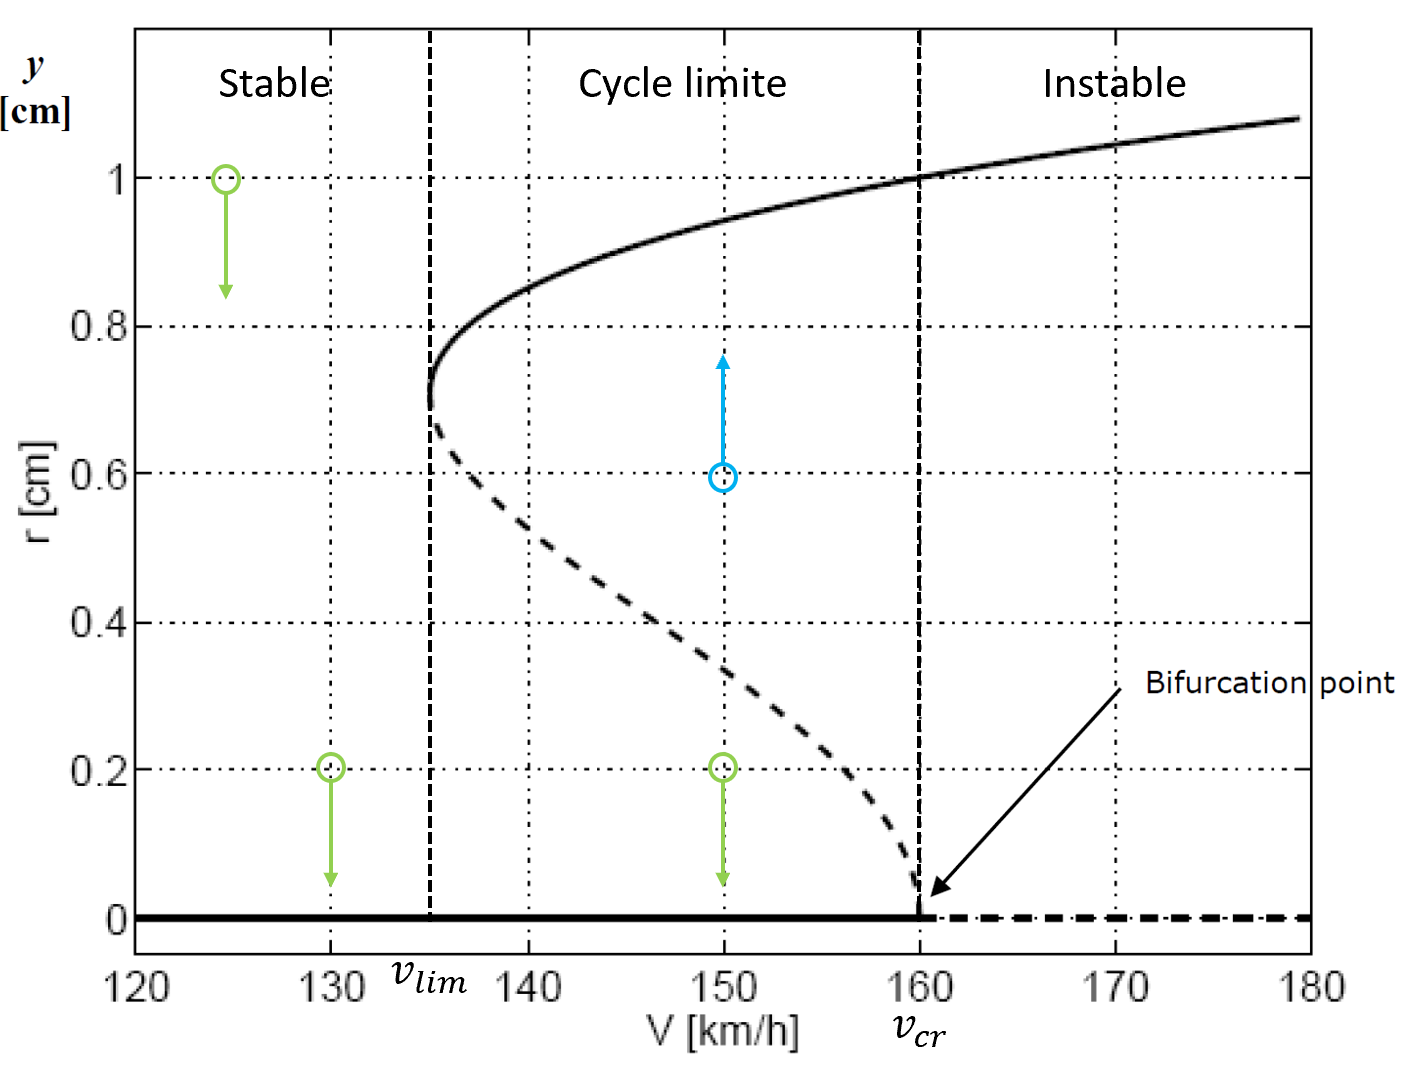
\includegraphics[scale=0.65]{Cycle_limite.png}
\end{figure}

En pratique, la vitesse du train sera limité à ne jamais dépasser sa vitesse limite afin d'éviter tout problème.


\section{MBS ferroviaire}
Un essieu sur des rail a 4 degrés de libertés et 2 contraintes:
\begin{itemize}
    \item $x$ : longitudinal,
    \item $y$ : latéral,
    \item $\psi$ : lacet,
    \item $\gamma$ : rotation.
\end{itemize}
Une roue seule a 5 ddl et une contrainte: elle a un mouvement de roulis $\phi$ supplémentaire possible.
Les différents repères sont utiles afin de définir les contraintes de contact:
\begin{figure}[H]
    \centering
    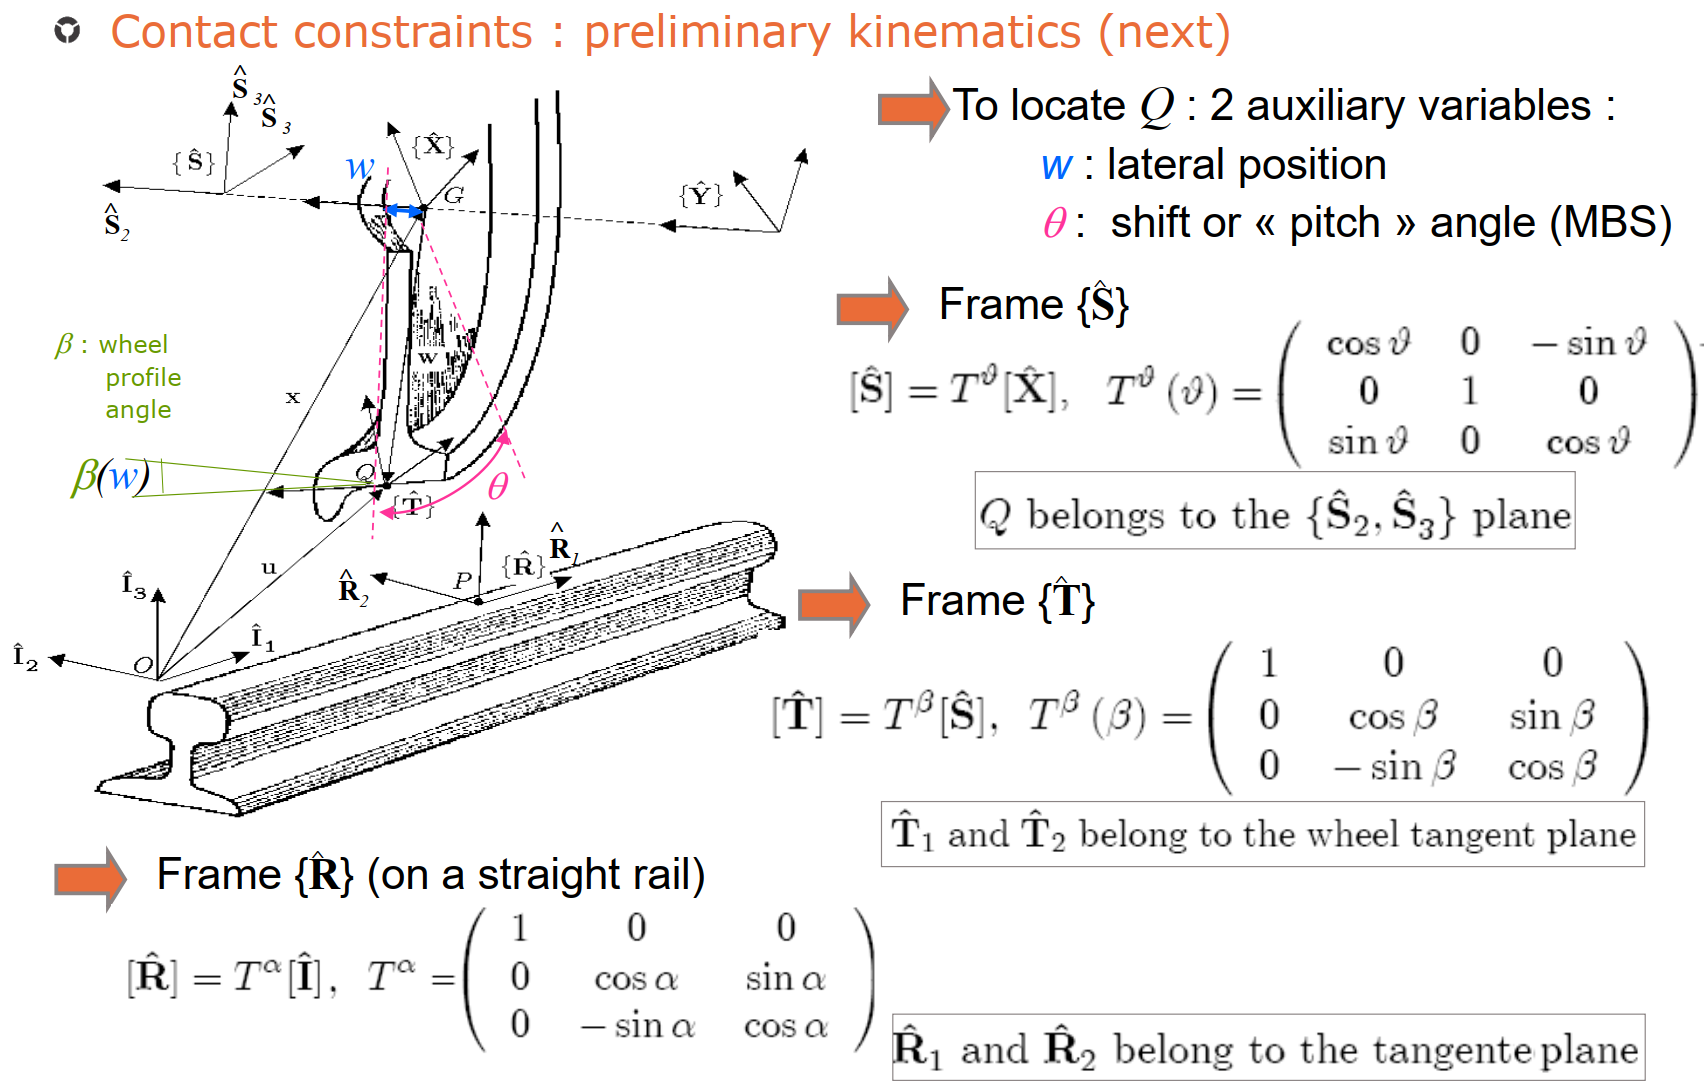
\includegraphics[width = 0.8\textwidth]{rail_mbs.PNG}
\end{figure}


Sachant que pour positionner un point de contact sur la roue, deux paramètres s'ajoutent ($w$ et $\theta$) le contact d'une seule roue s'exprime par les 3 contraintes suivantes:
\begin{align*}
    h_1(q,w,\theta) &= u_3 - \mu(u_2) = 0 \ \text{Le point de contact est sur le rail}\\
    h_2(q,w,\theta) &= \mathbf{\hat{T}_3} \cdot \mathbf{\hat{R}_1} = 0 \ \text{Tangence de la roue (perpendicularité T3 - R1)}\\
    h_3(q,w,\theta) &= \mathbf{\hat{T}_3} \cdot \mathbf{\hat{R}_2} = 0 \ \text{Tangence de la roue (perpendicularité T3 - R2)}\\
\end{align*}
Pour résoudre ces 3 contraintes, on fait appel à trois méthodes différentes. 
\begin{itemize}
    \item $h_1(q,w,\theta)$ est résolue en utilisant la méthode de Newton-Raphson comme c'est déjà le cas pour résoudre toute autre contraintes de système dynamique,
    \item $h_2(q,w,\theta)$ peut être résolu analytiquement. De fait, en utilisant les définitions des différents repères et en exprimant $\mathbf{\hat{T}_3}$ et $\mathbf{\hat{R}_1}$ dans $\mathbf{\hat{I}}$, la contrainte donne lieu à la relation suivante :
    \begin{equation*}
        R^G_{11}\sin{\theta} + R^G_{31}\cos{\theta} = R^G_{21}\tan{\beta} 
    \end{equation*}
    Qui a 2 solutions connues en $(\sin{\theta}, \cos{\theta})$ dont une mène à $\cos{\theta} < 0$ correspondant à un point de contact localisé sur la partie supérieur de la roue étant donc une solution non pertinente.
    \item $h_3(q,w,\theta)$ ne peut pas être calculée analytiquement. De la même manière que précédemment, on peut montrer que la contrainte se simplifie en l'expression suivante :
    \begin{equation*}
        \tan{\alpha} = -\frac{R^G_{12}\sin{\theta} - R^G_{22}\tan{\beta} + R^G_{32}\cos{\theta}}{R^G_{13}\sin{\theta} - R^G_{23}\tan{\beta} + R^G_{33}\cos{\theta}}
    \end{equation*}
    Qui n'a pas de solution analytique direct. Il faut donc obtenir cette solution numériquement. Cependant, pour des raison de problème de convergence, on n'utilise pas la méthode ne Newton-Raphson mais un méthode dichotomique.
\end{itemize}

\begin{figure}[H]
    \centering
    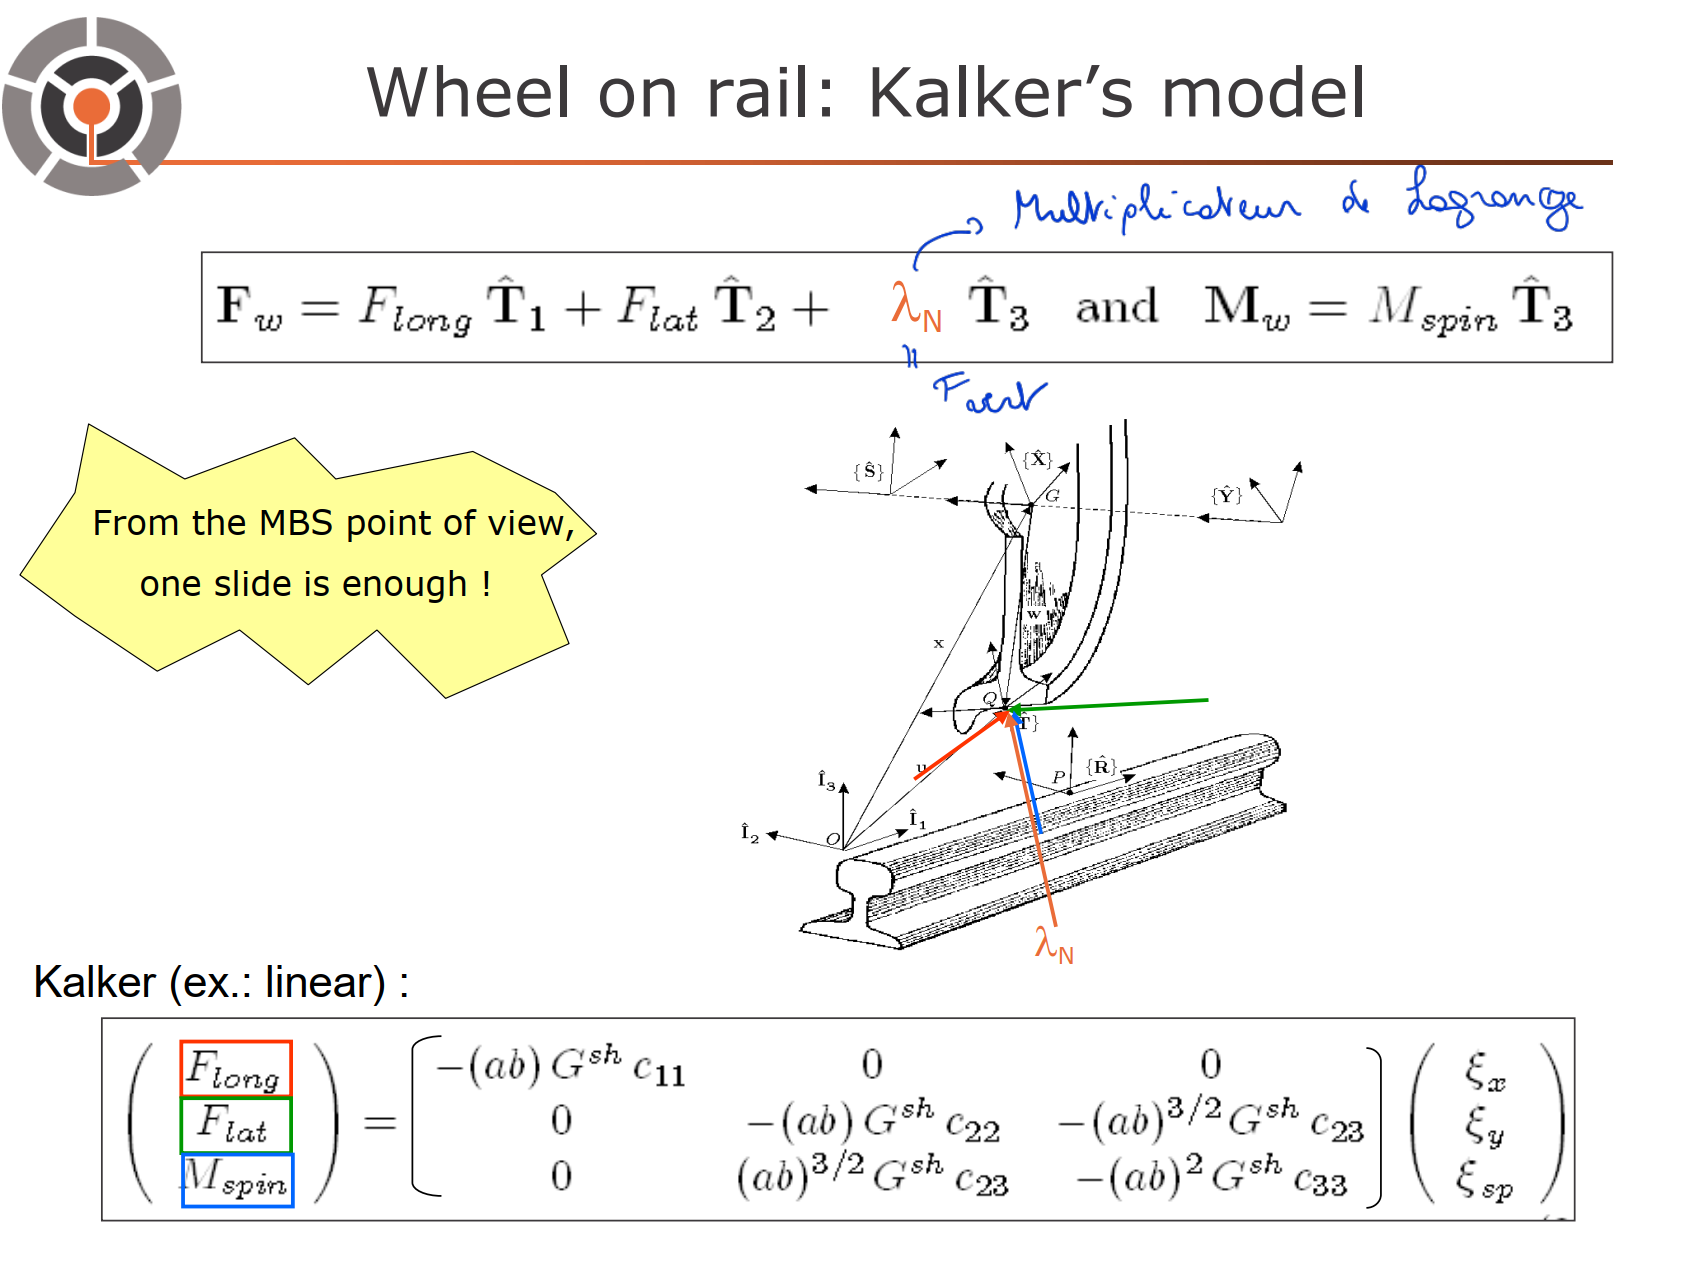
\includegraphics[width = 0.8\textwidth]{rail_mbs2.PNG}
\end{figure}



\paragraph{Implémentation du boudin de la roue:}
Il est possible de représenter le boudin comme un ressort-amortisseur qui entre en action si:
$$ y_{wheel} > y_{wheel-max} \ , \ F_{N-flange} = K_r \cdot (y_{wheel} - y_{wheel-max}) + D_r \cdot y_{wheel} \ ; \ \text{else     } F_{N-flange} = 0 $$
$$y_{wheel-max} \approx 6 \ mm \ , \ K_r \approx 1e^7 \ N/m \ , \ D_r \approx K_r / 100 \ N\cdot s/m $$

\section{Véhicules routiers :}
Les paramètres caractéristiques liés au châssis sont les suivant:
\begin{itemize}
    \item Basse fréquence :
    \begin{itemize}
        \item \textbf{Angle de roulis $\phi$:} $\dot{\phi}$ est le plus ressenti par les conducteurs, il est lié à la position de l'axe de roulis.
        \item \textbf{Angle de tangage $\gamma$ :} Bien maîtrisé par les suspensions et le long empattement. On parle de "cambrage" à l'accélération et de "plongée" au freinage.
    \end{itemize}
    \item Autres :
    \begin{itemize}
        \item \textbf{Angle de lacet $\psi$:} Aucun intérêt dynamique (comme $x$ et $y$) par contre $\dot{\psi}$ participe au caractère de conduite (entrée de courbe) et est utile pour le système d'ESP.
        \item \textbf{Angle de drift $\beta$:} Angle cinématique entre une position et une vitesse. Illustre le caractère globalement sur- ou sous- vireur du véhicule.
        \item \textbf{Empattement :} Distance entre essieux, influence le rayon de braquage. Ordre de grandeur $\approx 2.5 \ m$.
        \item \textbf{Voie :} Distance entre les roues d'un même essieu. Joue évidement sur la taille et l'habitabilité du véhicule. Influence la stabilité en roulis. Généralement identique à l'avant et à l'arrière. Ordre de grandeur $\approx 1.5 \ m$.
        \item \textbf{Pinçage (angle) :} Pincement ou ouverture. Si angle $> 0.5^{o}$: usure prématurée des pneus. Un léger pinçage en roulage est généralement bénéfique et améliore le temps de réponse du train avant (mais réduit la stabilité) parce qu'en virage la roue extérieure est "déjà" dans la courbe. Ordre de grandeur $\approx 0.2^o$ à l'avant.
        \item \textbf{Carrossage (angle) :} Généralement négatif ou contre-carrossage (plans des roues se croisent au-dessus du sol). Ordre de grandeur entre $0^o$ et $4^o$. Un carrossage négatif améliore la stabilité: tel un cône roulant sur le sol, une force pointe vers l'intérieur du véhicule. Utile en courbe !
        \item \textbf{Angle d'inclinaison de l'axe de pivot :}
        \begin{figure}[H]
            \centering
            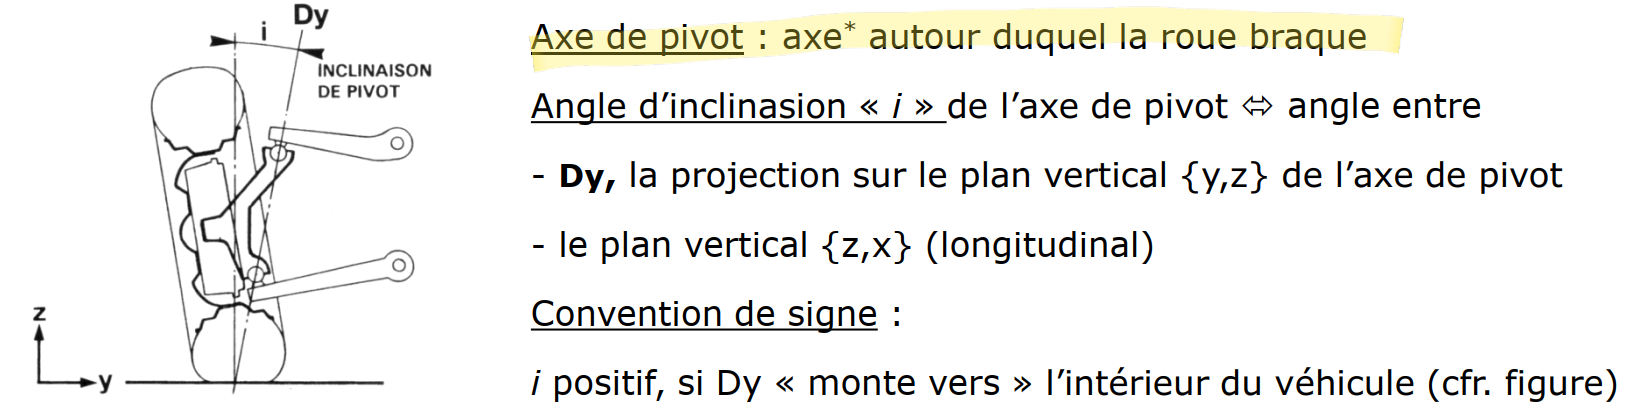
\includegraphics[width = 0.8\textwidth]{angle_pivot.PNG}
        \end{figure}
        
        
        Si l'angle positif, une rotation de la roue autour du pivot soulève le châssis $\rightarrow$ rappel gravitaire qui ramène en ligne droite. Ordre de grandeur $\approx 10^o \cdots 13^o$. Donne de la stabilité, mais implique des efforts de direction accrus!
        
        Le \textbf{déport au sol} (\autoref{deport}) est causé par l'angle de pivot. Un déport au sol négatif est stabilisateur en cas de freinage (\autoref{deport2}). Un déport nul est plus confortable aux chocs (car pas d'à-coups dans le volant) mais un déport non nul rend le braquage plus aisé (à l'arrêt).
        \begin{figure}[H]
            \begin{minipage}[b]{0.4\linewidth}   
            \centering
            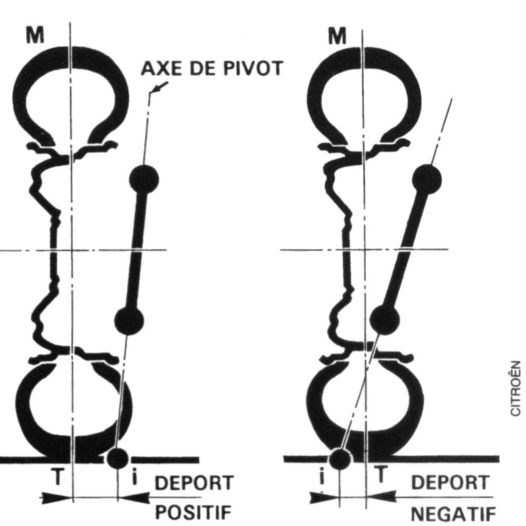
\includegraphics[width = 0.6\textwidth]{deport.PNG}
            \caption{Le déport au sol dépends de l'angle d'inclinaison de l'axe de pivot}
            \label{deport}
            \end{minipage}
            \hfill
            \begin{minipage}[b]{0.55\linewidth} 
            \centering
            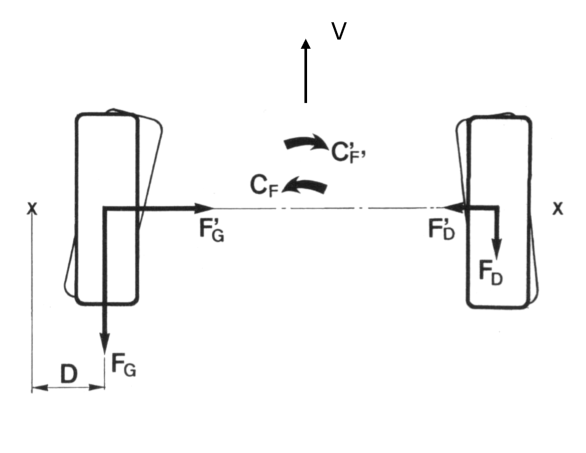
\includegraphics[width = 0.6\textwidth]{deport2.PNG}
            \caption{En cas de forces de freinages inégales, le déport au sol provoque un couple sur la direction qui s'oppose au couple provoqué par la différence entre les forces longitudinales.}
            \label{deport2}
            \end{minipage}
        \end{figure}
        
        \item \textbf{Angle de chasse de l'axe de pivot :} Ordre de grandeur $\approx +3 \cdots 4^o$.
        \begin{figure}[H]
            \centering
            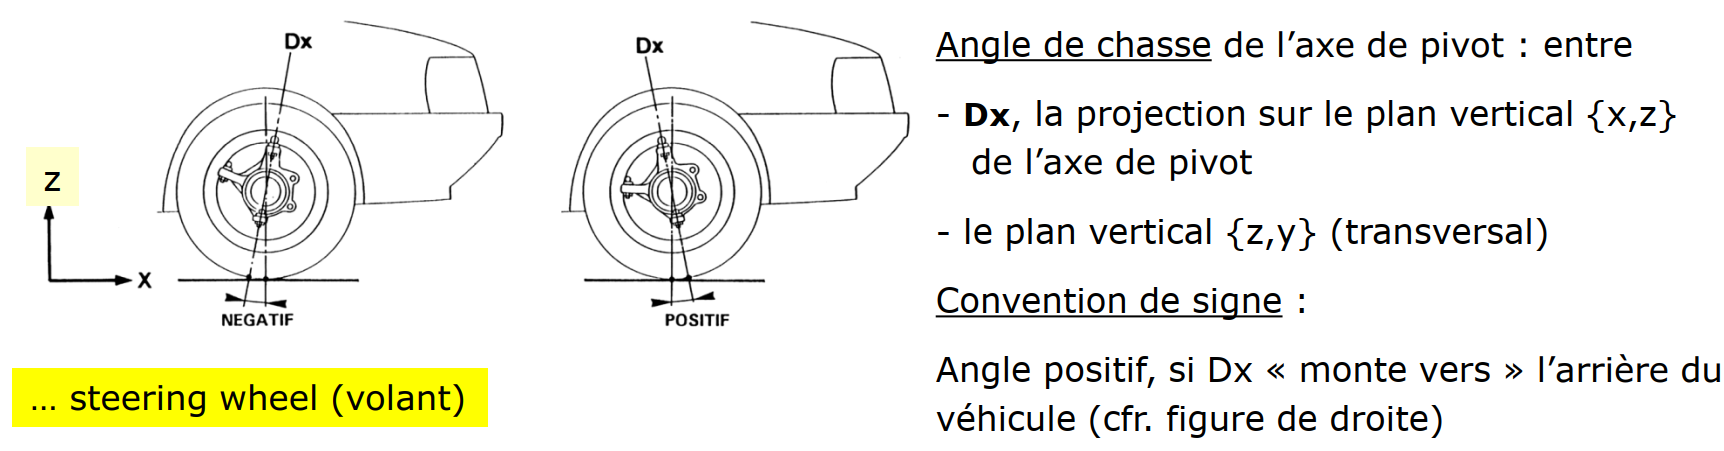
\includegraphics[width = 0.8\textwidth]{angle_chasse.PNG}
        \end{figure}
        
        L'angle de chasse est directement lié à \textbf{la chasse} qui est la distance entre le point de percée de l'axe de pivot avec le sol et le point de contact roue/sol. Une chasse positive a un effet auto-stabilisateur car la force de contact tend à ré-aligner la roue (comme une roue de caddie). Un désavantage est l'apparition d'un rappel gravitaire inversé = instabilité (comme la fourche d'une moto ou d'un vélo qui tombe toute seule d'un côté ou de l'autre à basse vitesse).
        \item \textbf{Angle de dérive $\alpha$:} Angle formé par l'intersection de:
        \begin{itemize}
            \item l'intersection du plan médian de la roue et du sol
            \item la projection du vecteur vitesse du centre de la roue dans le plan du sol
        \end{itemize}
        
        \begin{figure}[H]
            \centering
            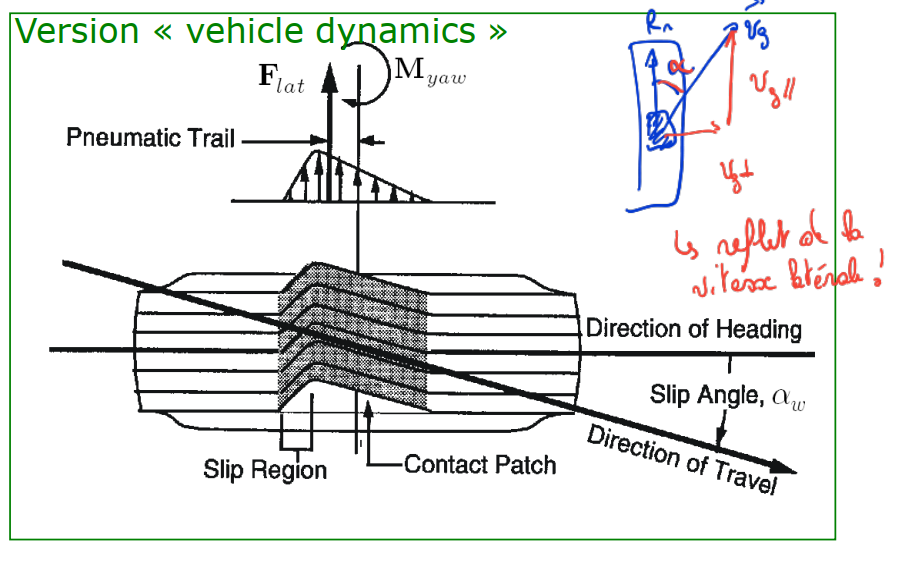
\includegraphics[width = 0.5\textwidth]{angle_slip.PNG}
        \end{figure}
        \vspace{-0.5cm}
        \item \textbf{Centre de roulis (CR):} Centre instantané de rotation (CIR) du châssis par rapport au sol, définit dans le plan transversal $\{y,z\}$ au droit d'un essieu.
        
        Une manière pratique pour l'évaluer est d'appliquer une force sur la "bisectrice" de l'essieu et de la déplacer jusqu'à ce qu'elle ne provoque plus de mouvement de roulis du châssis.
        Le \textit{théorème de Kennedy} permet de trouver le centre de roulis rapidement en stipulant que celui-ci est alligné avec le CIR roue/châssis et le CIR roue/sol.
         \item \textbf{Axe de roulis :} Axe reliant les deux centres de roulis des essieux.
    \end{itemize}
\end{itemize}

\paragraph{Épures cinématiques et élastocinématiques:}
L'épure \textbf{cinématique} observe l'évolution de la demi-voie, du carrossage, du parallélisme et de l'empattement pour différentes hauteurs de caisses. Cela permet d'étudier comment ces paramètres change lorsque les suspensions "travaillent".
L'étude \textbf{élastocinématique} présente le même type de résultats, mais issus d'équilibres quasi-statiques.

\subsection{Transfert de charge}
Afin de pouvoir calculer le transfert de charge en ligne droite, on peut utiliser le principe des puissances potentielles ou PPP (notons qu'il est parfaitement possible de s'en passer en utilisant un équilibre des forces et des masses ! ).

\begin{equation}\label{eq:ppp}
    \sum_{i=1}^N \Big ( m^i \mathbf{\ddot{x}}^i - \mathbf{F}^i \Big) \cdot \Delta \mathbf{\dot{x}}^i + \sum_{i=1}^N \Big (  \mathbf{\dot{H}}^i - \mathbf{L}^i \Big) \cdot \Delta \mathbf{\dot{\omega}}^i = 0
\end{equation}
Où $\Delta \mathbf{\dot{x}}^i$ et $\Delta \mathbf{\dot{\omega}}^i$ sont des changement virtuels de vitesses. Ceux-ci peuvent être :
\begin{itemize}
    \item \textbf{Compatible} avec les contraintes de sorte que (par exemple):
    \begin{gather*}
        \Delta \mathbf{\dot{x}} = \Delta \dot{q} \mathbf{\hat{X}}_j\\
        ( m \mathbf{\ddot{x}} - \mathbf{F}) \cdot \Delta \dot{q} \mathbf{\hat{X}}_j = 0
    \end{gather*}
    \textit{La contribution de toute force ou couple de contrainte au changement virtuel de puissance est nulle pour tout choix de changement virtuel de vitesse compatible avec les contraintes.}
    
    \item \textbf{Non compatible} avec une ou plusieurs contraintes. Un tel choix va donc faire apparaître la contribution de la (des) force(s) liée(s) avec la (les) contraintes non respectée(s).
\end{itemize}

\paragraph{\textbf{Cas d'une voiture "monobloc", donc avec suspension rigide :}} Dans notre cas, on souhaite faire apparaître la force de contrainte sol/roue avant et arrière. Pour se faire, un choix \textbf{non compatible} de vitesse virtuelle serait :
\begin{itemize}
    \item Pour faire apparaître la force de contact sol/roue avant serait $\Delta \mathbf{\dot{x}} = \Delta \overrightarrow{\Omega}_{O_{AR}} \mathbf{\Hat{I}_2}$ et $\Delta \mathbf{\dot{\omega}} = 0$ pour ne faire apparaître que la force. On fait donc tourner la voiture autour de $O_{AR}$. 
    
    Les PPP (\ref{eq:ppp}) se réécrivent :
    \begin{equation*}
        \sum_{i=1}^N \Big ( m^i \mathbf{\ddot{x}}^i - \mathbf{F}^i \Big) \cdot \Delta \mathbf{\dot{x}}^i = 0
    \end{equation*}
    Avec :
    \begin{equation*}
        \Delta \mathbf{\dot{x}}^i = \Delta \overrightarrow{\Omega}_{O_{AR}} \mathbf{\Hat{I}_2} \times  \overrightarrow{O_{AR}O_i}
    \end{equation*}
    Où $\overrightarrow{O_{AR}O_i}$ définit le vecteur position entre $O_{AR}$ et le centre de masse du corps i (car $O_{AR}$ est un point fixe) .
    
    \item Pour faire apparaître la force de contact sol/roue arrière serait $\Delta \mathbf{\dot{x}} = \Delta \overrightarrow{\Omega}_{O_{AV}} \mathbf{\Hat{I}_2}$ et $\Delta \mathbf{\dot{\omega}} = 0$ pour ne faire apparaître que la force. On fait donc tourner la voiture autour de $O_{AV}$. 
    
    Les PPP (\ref{eq:ppp}) se réécrivent :
    \begin{equation*}
        \sum_{i=1}^N \Big ( m^i \mathbf{\ddot{x}}^i - \mathbf{F}^i \Big) \cdot \Delta \mathbf{\dot{x}}^i = 0
    \end{equation*}
    Avec :
    \begin{equation*}
        \Delta \mathbf{\dot{x}}^i = \Delta \overrightarrow{\Omega}_{O_{AV}} \mathbf{\Hat{I}_2} \times  \overrightarrow{O_{AV}O_i}
    \end{equation*}
    Où $\overrightarrow{O_{AV}O_i}$ définit le vecteur position entre $O_{AV}$ et le centre de masse du corps i (car $O_{AV}$ est un point fixe).
\end{itemize}

Sur base de calculs de PPP ou de plusieurs équilibres Forces/Moments on peut déterminer la répartitions des masses en 2D comme la somme d'un force statique due au poids et d'un terme de charge qui dépendra de l'accélération du véhicule $\ddot{R}$ :
\begin{figure}[H]
    \centering
    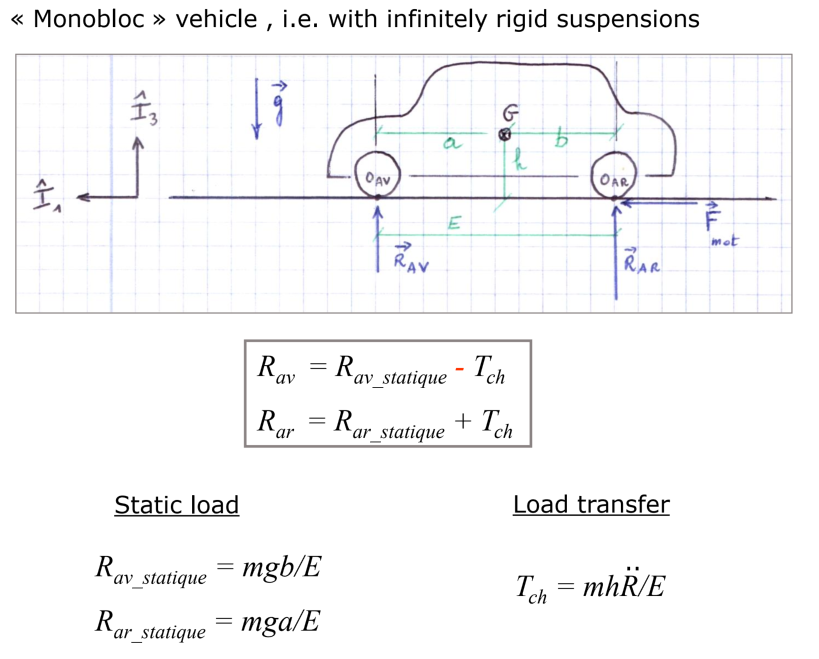
\includegraphics[width = 0.6\textwidth]{load_transfert.PNG}
\end{figure}

On peut en faire de même latéralement, avec $\ddot{q} = \Omega^2 \, R$ l'accélération centripète et $v$ la voie :

\begin{minipage}{0.6 \textwidth}
    \begin{figure}[H]
        \centering
        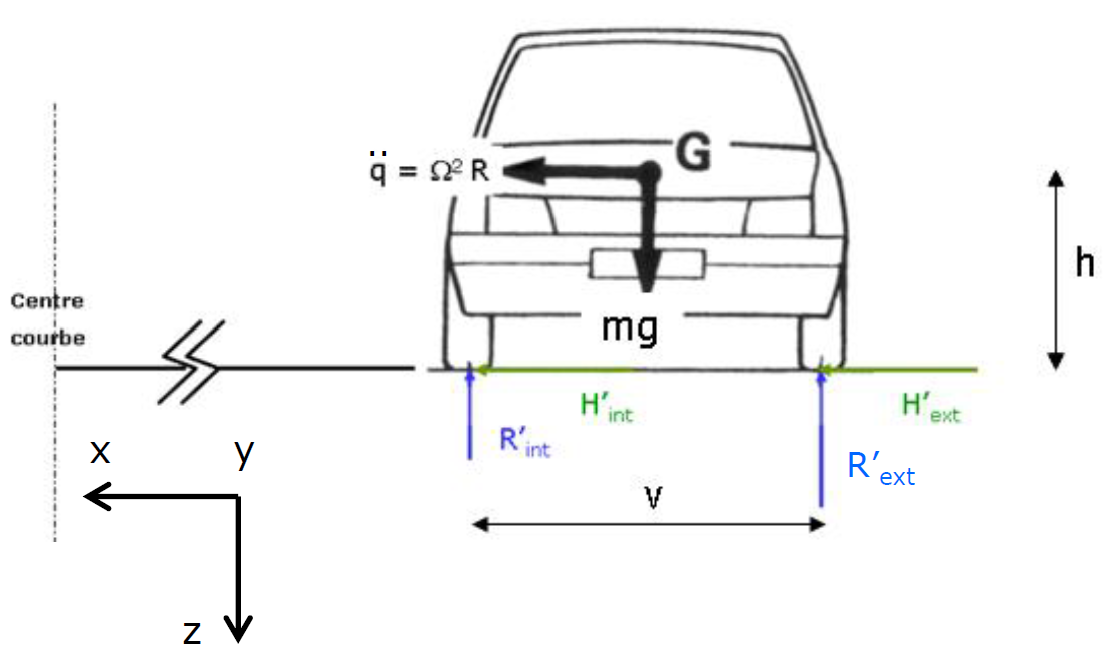
\includegraphics[scale=0.6]{transfert_lat.png}
    \end{figure}
\end{minipage}
\hspace{1cm}
\begin{minipage}{0.35 \textwidth}
    \begin{align*}
        R_{int} &= \cfrac{m g}{2} - \cfrac{m h \ddot{q}}{v}\\
        R_{ext} &= \cfrac{m g}{2} + \cfrac{m h \ddot{q}}{v}
    \end{align*}
\end{minipage}

Où le terme de transfert de charge est bien $T_{ch} = \cfrac{m h \ddot{q}}{v}$.

\paragraph{\textbf{Cas d'une voiture avec suspension en roulis dans un tournant :}} Dans le cas d'un virage ( donc avec du roulis $\phi$) la technique reste toujours la même mais nécessite d'avantage de paramètres et de forces en jeu. De fait, pour obtenir le transfert de charge de ce véhicule, on procède en 3 équilibres :

\begin{enumerate}
    \item Équilibre latéral, vertical et de roulis de l'essieu avant :
    \begin{eqnarray*}
        &y& : F_1^{ext} + F_1^{int} - F_1^{e} = m^e q^e\\ 
        &z& : N_1^{ext} + N_1^{int} = P_1^e \Rightarrow N_1^{ext} \triangleq \frac{P_1^{e}}{2} + T_1 \text{ \& } N_1^{int} \triangleq \frac{P_1^{e}}{2} - T_1\\
        &\phi& : K_1\phi + N_1^{int}\frac{v_1}{2} - N_1^{ext}\frac{v_1}{2} + F_1^e h_1 = 0
    \end{eqnarray*}
    \vspace{-0.5cm}
    \item Équilibre latéral et de lacet du châssis :
    \begin{eqnarray*}
        &\psi& : F_1^{ch}a_1 - F_2^{ch}a_2 = 0\\ 
        &y& : F_1^{ch} + F_2^{ch} = m^{ch} q^{ch}
    \end{eqnarray*}
    \vspace{-0.5cm}
    \item Équilibre en roulis du châssis :
    \begin{equation*}
        \phi : M_1^{ch} + M_2^{ch} - F_1^{ch} (H' + \Delta h) - P_1^{ch} (H' + \Delta h)\phi - F_2^{ch} (H' - \Delta h) - P_2^{ch} (H' - \Delta h)\phi
    \end{equation*}
\end{enumerate}

\begin{figure}[H]
    \centering
    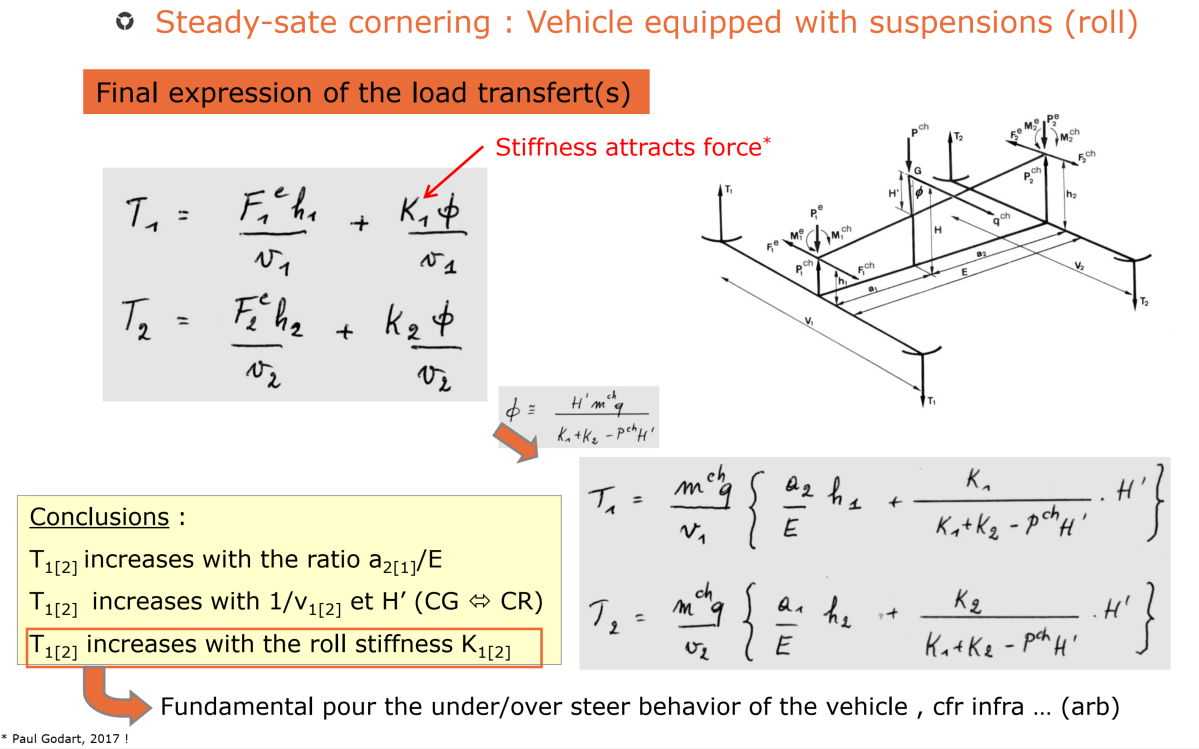
\includegraphics[width = 0.8\textwidth]{load_transfert3D.PNG}
\end{figure}

Notons que les équations ci-dessus permettent d'observer l'impact d'une barre anti-roulis qui augmenterai les raideurs en roulis $K_1$ et $K_2$.
Une barre anti-roulis rend une voiture sous-vireuse car augmente $K_1$ et/ou $K_2$ donc augmente $T_1$ et/ou $T_2$ ce qui augmente la charge du côté extérieur de la voiture ayant pour conséquence de faire moins tourner la voiture.

\begin{figure}[H]
    \centering
    \includegraphics[scale=0.2]{sous_sur_vireuse.jpg}
\end{figure}

$F_{lat,moyen}$ plus petit si K augmente donc $a_{centrip\grave{e}te}$ plus petite. Or, $a_{c} = \omega^2 R = \frac{v^2}{R}$ si v est inchangé (car même configuration) alors R doit augmenter $\Rightarrow$ sous-vireuse. 

\subsection{Morphologies d'essieu :}
\paragraph{Mc Pherson}
Le Mc Pherson intégral est une structure quelque-peu minimaliste dans laquelle le ressort-amortisseur à également un rôle de guidage (ce qui implique un sur-dimensionnement de celui-ci) car la fusée y est solidaire. Le bras de suspension est simple ce qui impose d'utiliser la barre anti-roulis pour le guidage. 'axe de braquage de la roue est formé par un pivot entre le bras de suspension et la fusée et le point d'appuis supérieur du ressort-amortisseur $\Rightarrow$ deux organes de suspension participent donc au guidage !
\begin{figure}[H]
        \begin{minipage}[b]{0.40\linewidth}   
        \centering
        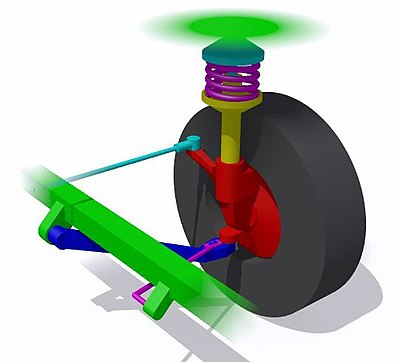
\includegraphics[width = \textwidth]{McPherson.jpg}
        \caption{Vue schématique du McPherson intégral. (turquoise) bielle de direction, (bleu) bras de suspension, (rouge) fusée, (mauve) barre anti-roulis.}
        \label{McPherson}
        \end{minipage}
        \hfill
        \begin{minipage}[b]{0.55\linewidth} 
        \centering
        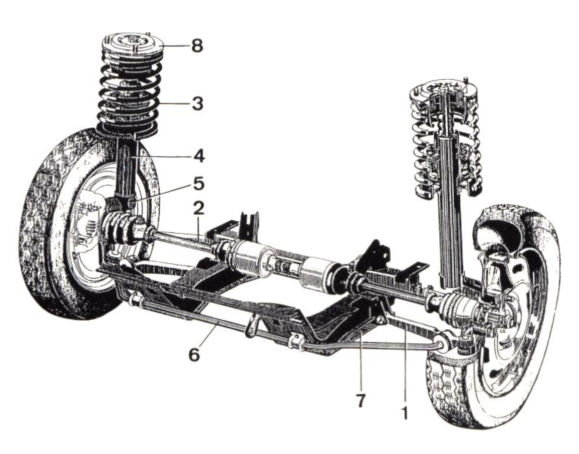
\includegraphics[width = \textwidth]{McPherson.PNG}
        \caption{(1) bras de suspension, (2) bielle de direction, (3-4) ressort-amortisseur, (5) fusée, (6) barre anti-roulis, (7) châssis, (8) Appuis supérieur à bille.}
        \label{McPherson2}
        \end{minipage}
\end{figure}
    Les avantages se situent dans la simplicité et la compacité (donc un prix plus bas) du système. Cependant, le guidage est médiocre, les épures limitées et des frottements ont lieu dans la suspension.
\paragraph{Pseudo McPherson}
Le principe est le même mais la bielle de suspension est remplacée par un triangle, ce qui permet de décharger la barre anti-roulis du guidage.

\begin{figure}[H]
        \begin{minipage}[b]{0.45\linewidth}   
        \centering
        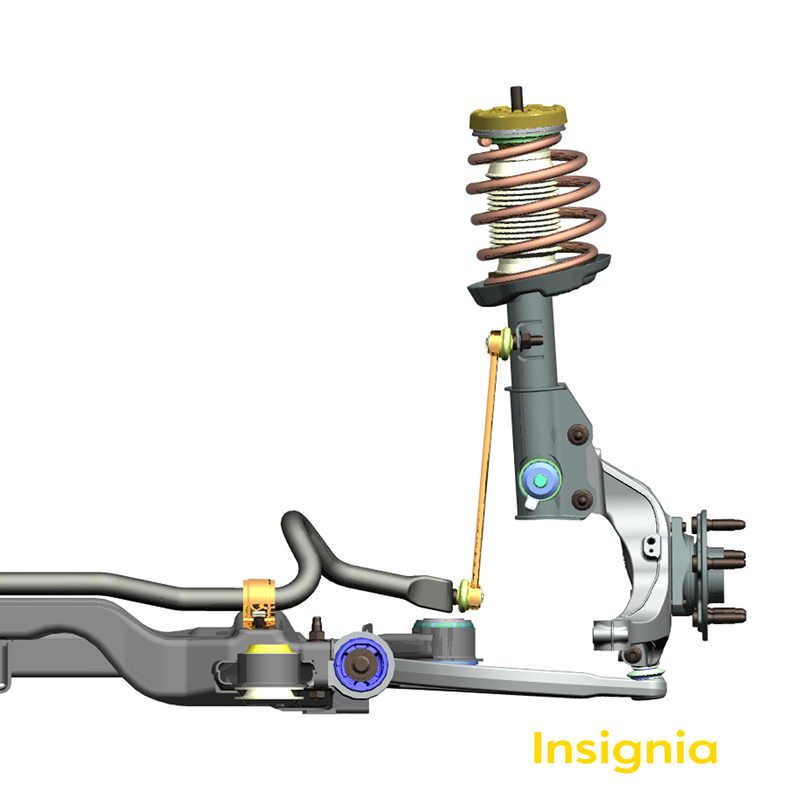
\includegraphics[width = \textwidth]{Pseudo-Mac-Pherson.jpg}
        \caption{Pseudo-MacPherson : vue de la biellette reliant la barre anti-roulis au ressort-amortisseur.}
        \label{PseudoMcPherson}
        \end{minipage}
        \hfill
        \begin{minipage}[b]{0.45\linewidth} 
        \centering
        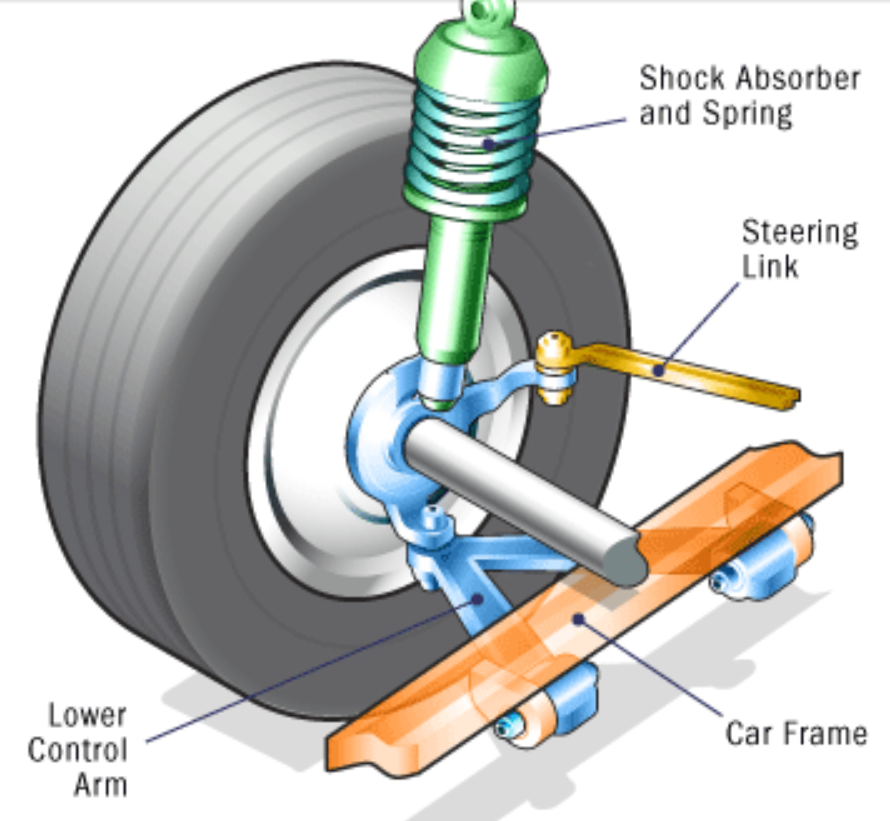
\includegraphics[width = \textwidth]{Pseudo-Mac-Pherson.png}
        \caption{Pseudo-MacPherson : vue du triangle de suspension (en bleu) et de la façon la bielle de direction vient s'attacher à la fusée.}
        \label{PseudoMcPherson2}
        \end{minipage}
\end{figure}
Il 'agit d'un des essieux les plus utilisés dans les voiture de tourisme ! Le guidage des roues est bon et il reste simple et compact (peu cher).

\paragraph{Essieu anti-cabreur, anti-plongée :}
Pour un macpherson, mais aussi pour d'autres types de suspensions. Il se réalise en inclinant vers l'avant l'axe du bras (triangle) de suspension (sur le schéma ci-dessous: 3 et 4 = axe de rotation, 5 = triangle de suspension).
\begin{itemize}
    \item Lors de la compression la rotule (2) monte et avance,
    \item Lors de la détente la rotule (2) descend et recule.
\end{itemize}
\begin{figure}[H]
    \centering
    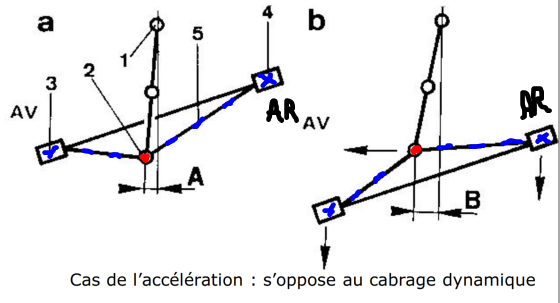
\includegraphics[width = 0.5\textwidth]{anti_cabreur.PNG}
\end{figure}

Dynamiquement la force horizontale lors d'une accélération/d'un freinage tends à s'opposer au cabrage/plongée. Mais lors de la prise d'une bosse l'effet nuit au confort. $\rightarrow$ compromis à trouver !


\paragraph{Pseudo-MacPherson à pivot indépendant :}
Encore une amélioration du MacPherson... ! Création d'un axe de pivot ( pour le braquage de la roue) indépendant de la suspension. Le ressort-amortisseur ne tourne plus. Cela permet de découpler les réglages du pivot de l'épure (demi-voie, carrossage, centre de roulis).
\begin{figure}[H]
        \begin{minipage}[b]{0.4\linewidth}   
        \centering
        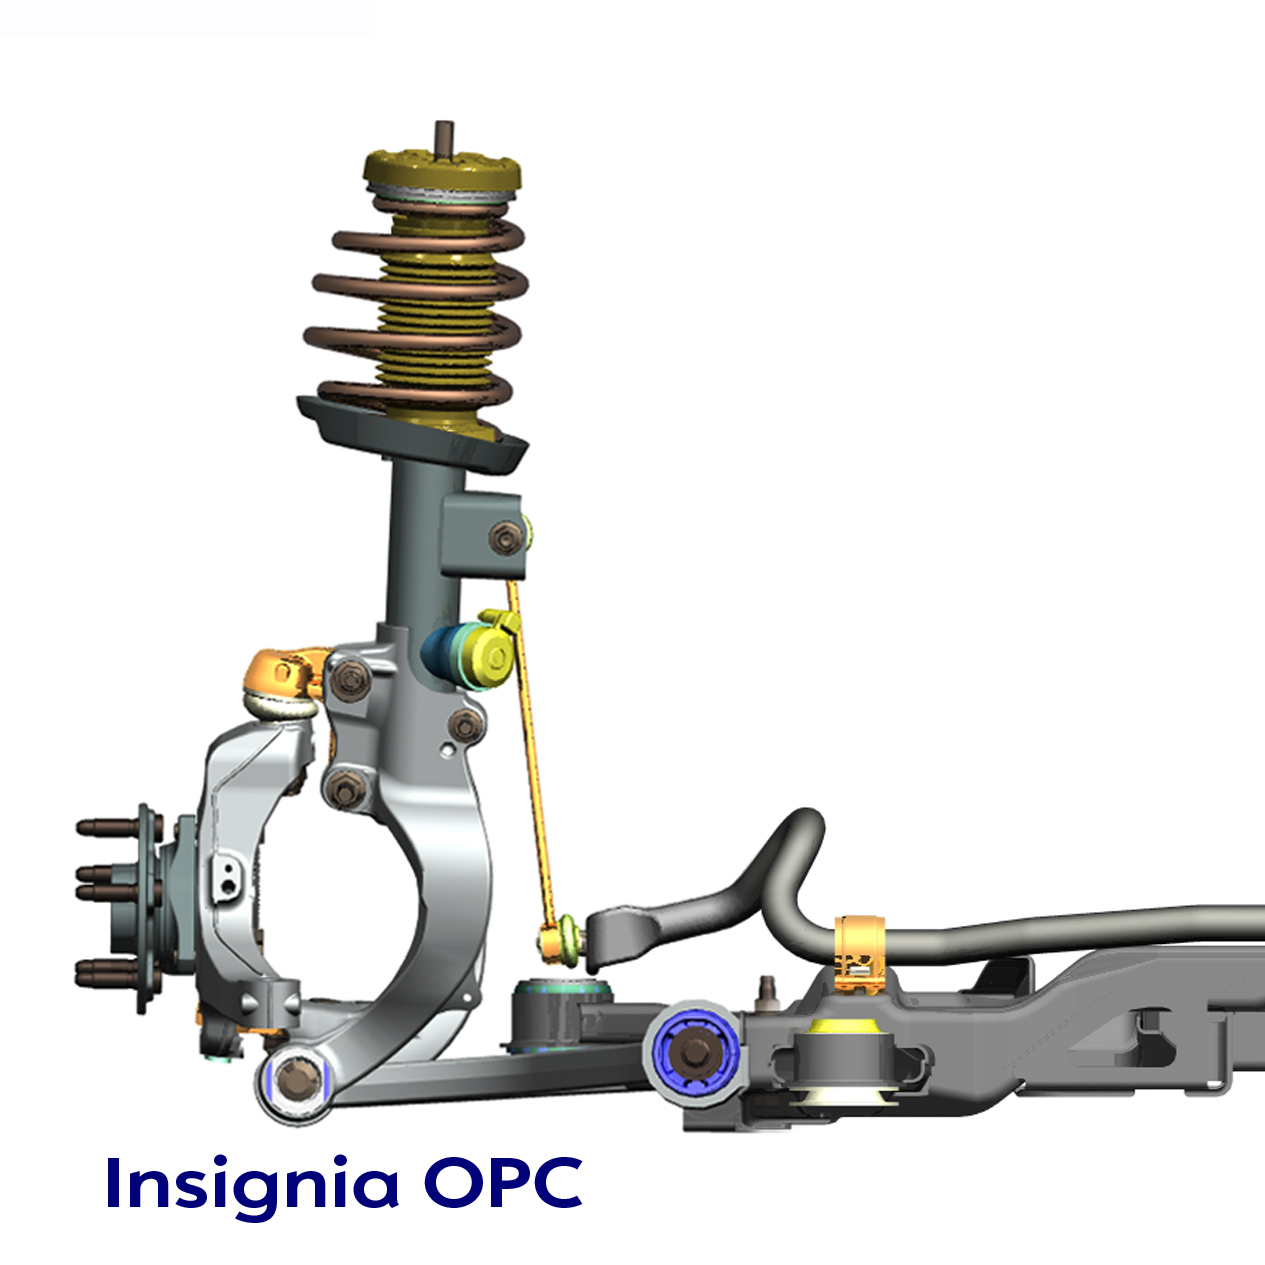
\includegraphics[width = \textwidth]{Pseudo-Mac-Pherson-Pivot-Independant.jpg}
        \caption{Pseudo-MacPherson à pivot indépendant.}
        \label{PseudoMcPhersonInd}
        \end{minipage}
        \hfill
        \begin{minipage}[b]{0.55\linewidth} 
        \centering
        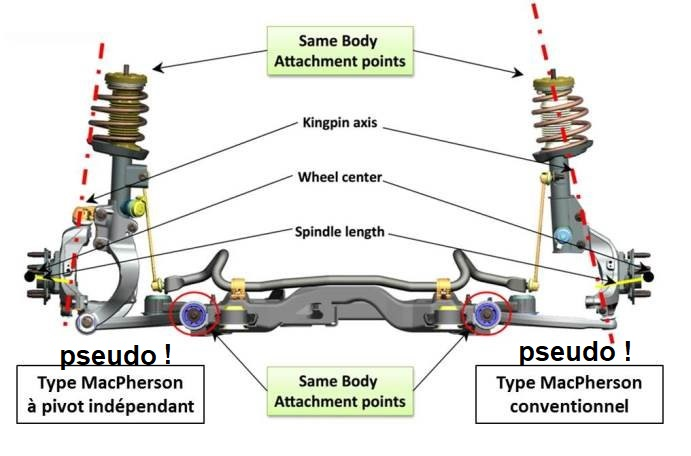
\includegraphics[width = \textwidth]{pivot_independant.jpg}
        \caption{Comparaison Pseudo MacPherson et Pseudo MacPherson à pivot indépendant.}
        \label{PseudoMcPhersonInd2}
        \end{minipage}
\end{figure}


\paragraph{Rôle de la barre anti-roulis :}
La barre anti-roulis augmente la raideur en roulis entre la caisse et l'essieu. La barre agit comme un ressort en torsion. Elle ne modifie cependant pas la raideur en pompage. Le montage peut se faire sur le triangle ou sur l'élément porteur (comme dans la \autoref{PseudoMcPherson2}). L'inconvénient est qu'elle engendre des mouvements de roulis lors du passage d'obstacles asymétrique (un compromis dois donc être fait) et tend à rendre une voiture sous-vireuse.

\paragraph{Essieux à bras superposés :}
Comme le nom l'indique, deux bras s'occupent du guidage de sorte que le ressort-amortisseur fait uniquement le soutien. Ils sont très bon en guidage et permettent des réglages simples des épures. L'inconvénient est l'encombrement transversal et le prix de reviens.

\paragraph{Essieu multi-bras :}
La fusée est reliée au châssis par plusieurs bielles. Peuvent être très différents en fonctions des configurations choisies.

\paragraph{Essieux rigides :}
Capacité de charge, robustesse et aspect "économique" avant l'agrément de conduite. Les roues sont reliées rigidement par l'essieu qui est relié à la caisse par des ressorts à lame ou un système de bielles et de ressorts.

\paragraph{Essieux à bras tirés :}
Essieux rigide en flexion mais souple en torsion tiré par des bras reliés à la caisse.
Notons qu'une variante où les roues sont indépendante est possible (exemple: VW Sharan 2009).

\paragraph{Essieux directionnels :}
\begin{itemize}
    \item Version passive, sans actionneur, où tout est géré par un choix judicieux des éléments élastiques.
    \item Version active, lié à la rotation du volant.
    \item Version active avec actionneurs électro-hydrauliques et capteurs.
\end{itemize}

\section{Contact pneu/sol :}
Le contact est implémenté comme une force résultante de la position et du mouvement du pneu par rapport au sol.
Les phénomènes physiques en jeu sont:
\begin{itemize}
    \item Glissement et frottement dans la zone de contact,
    \item Déformation du pneu.
\end{itemize}
Deux angles sont importants pour la suite: l'angle de carrossage $\gamma$ et l'angle de glissement ou drift $\alpha$.
\textbf{Attention :} il y a deux normes pour le système d'axe utilisé : SAE avec l'axe $\overrightarrow{z}$ vers le bas et ISO avec l'axe $\overrightarrow{z}$ vers le haut. 
Voici ci-dessous les noms des différentes forces et couples en jeu :
\begin{figure}[H]
    \centering
    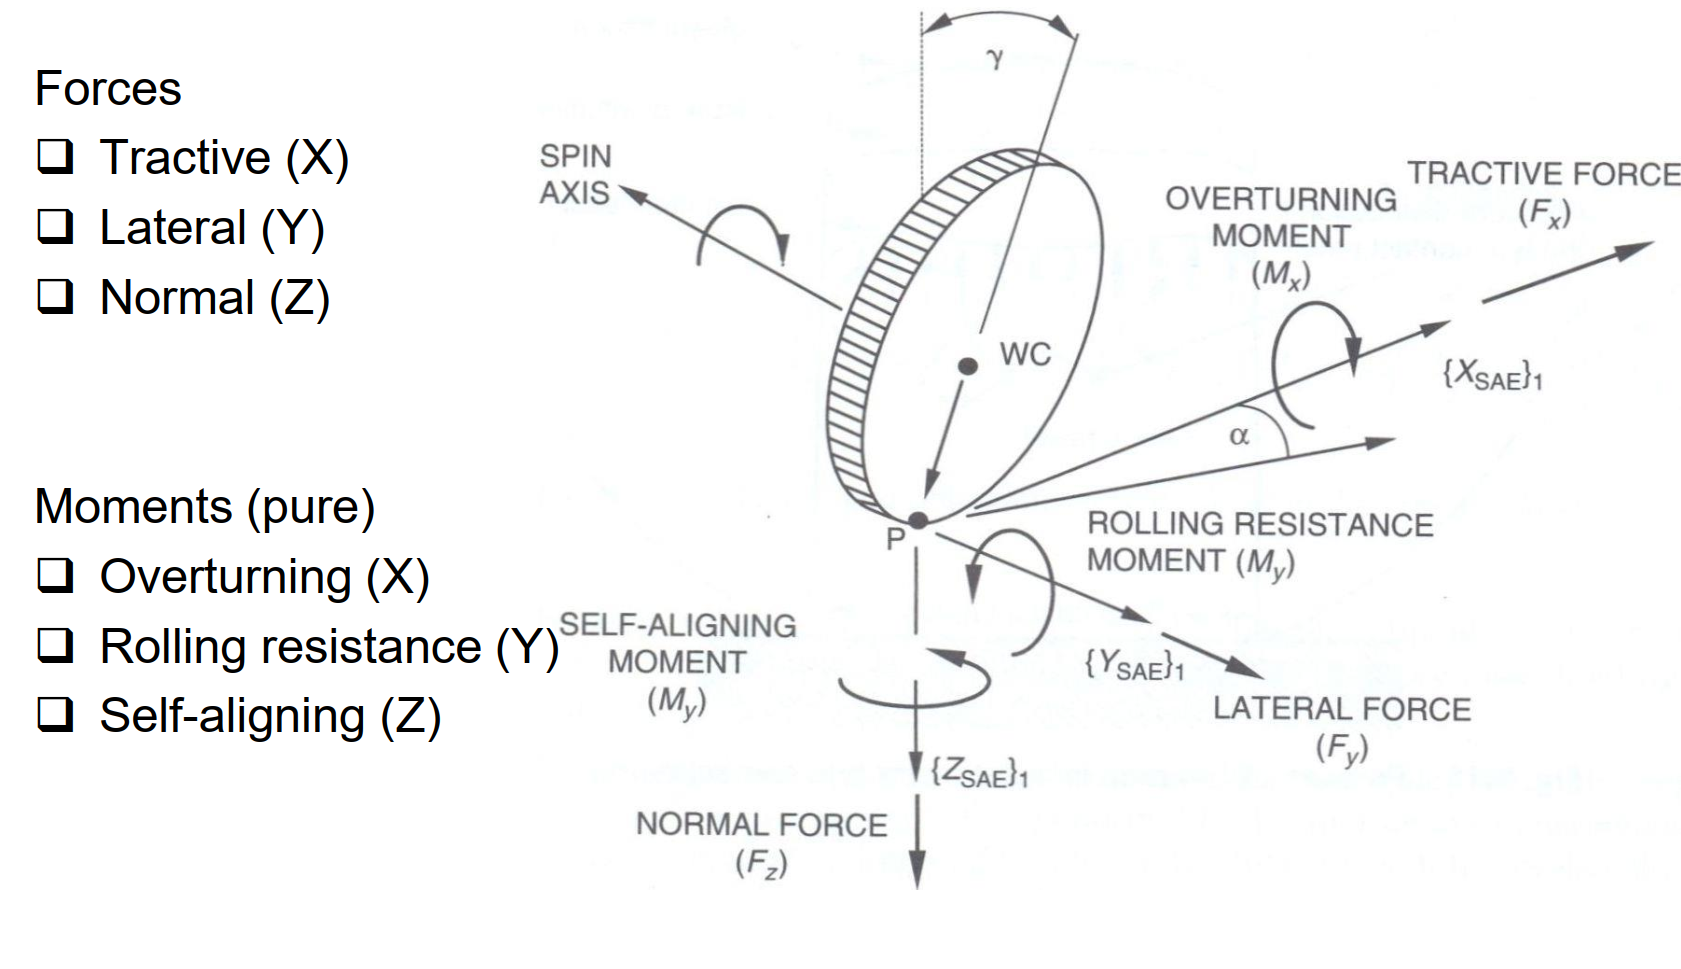
\includegraphics[width = 0.6\textwidth]{contact_pneu.PNG}
\end{figure}

\paragraph{Force normale :} On considère le pneu comme un ressort-amortisseur,

\paragraph{Résistance au roulement :} La résistance au roulement est égale à la force verticale $F_V$ multipliée par un coefficient de frottement $\mu_R$ : $F_R = \mu_R \cdot F_V$.

\paragraph{Phénomène du frottement :} 
Un pneu sur le sol est un contact non-ponctuel, ce qui implique du glissement dans la surface de contact. De plus, le pneu se déforme : l'avant du pneu se comprime lorsque l'arrière se détend. Donc frottements inter-cristallins = dissipation d'énergie cinétique. Par ailleurs, les éléments composant le pneu ne se déforme pas de la même manière en compression et en détente. 

\begin{equation*}
    F_{d\acute{e}tente} < F_{compression}
\end{equation*}

Cette différence va alors entraîner un couple de freinage.

\begin{figure}[H]
    \centering
    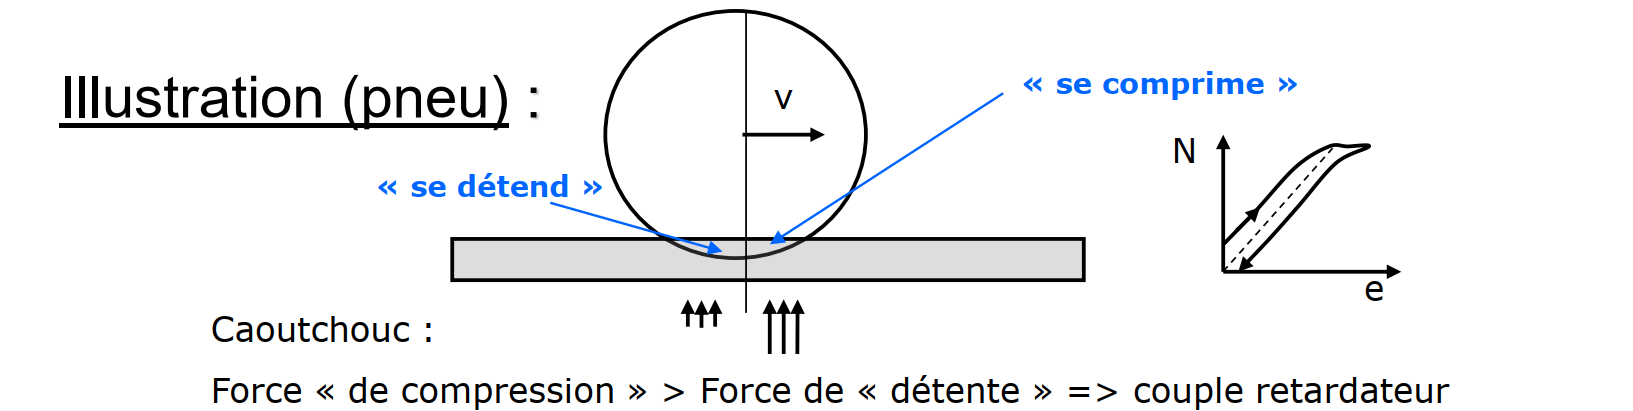
\includegraphics[width = 0.8\textwidth]{contact_pneu2.PNG}
\end{figure}

\paragraph{Pure cornering, braquage simple :} pas d'accélération/freinage, pas de carrossage. L'angle de drift provoque une force latérale et un couple d'alignement.
\begin{figure}[H]
    \centering
    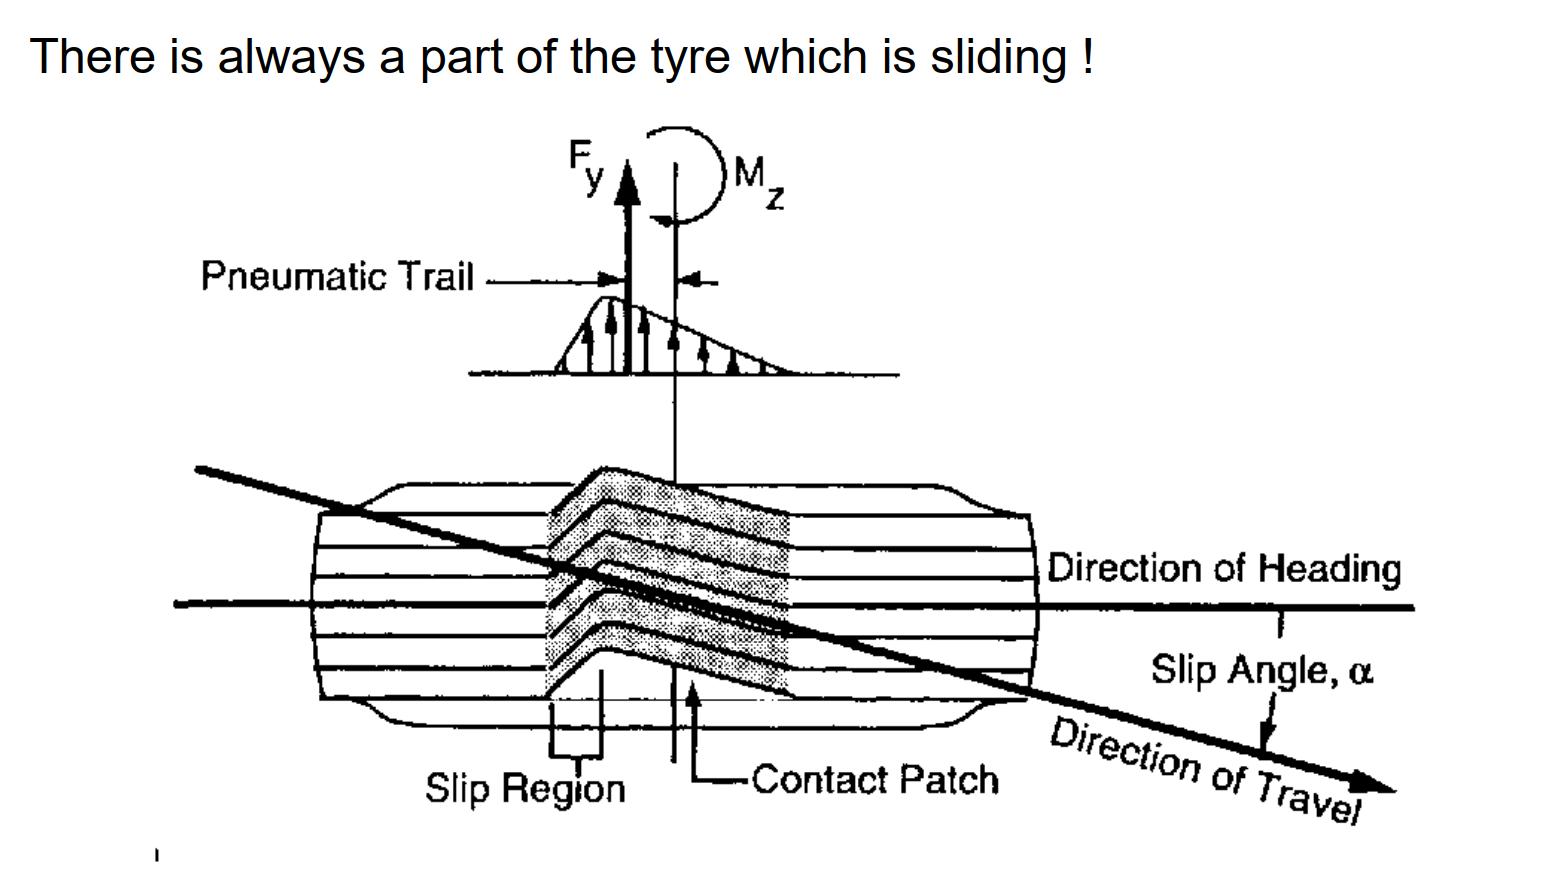
\includegraphics[width = 0.6\textwidth]{contact_pneu3.PNG}
    \caption{Modèle de Calspan}
    \label{Calspan}
\end{figure}

Le modèle de \textbf{Fromm} donne une explication sur la force latéral et le moment auto-stabilisateur dû à l'angle de glissement basé sur l'hypothèse que le pneu se comporte comme une série de ressort latéraux.

\begin{equation*}
    F_y = (C_y \cdot \Delta x) \cdot \delta(x)    
\end{equation*}

Avec $C_y$ en $[N/(m_xm_y)]$.

\vspace{-0.5cm}
\begin{figure}[H]
    \centering
    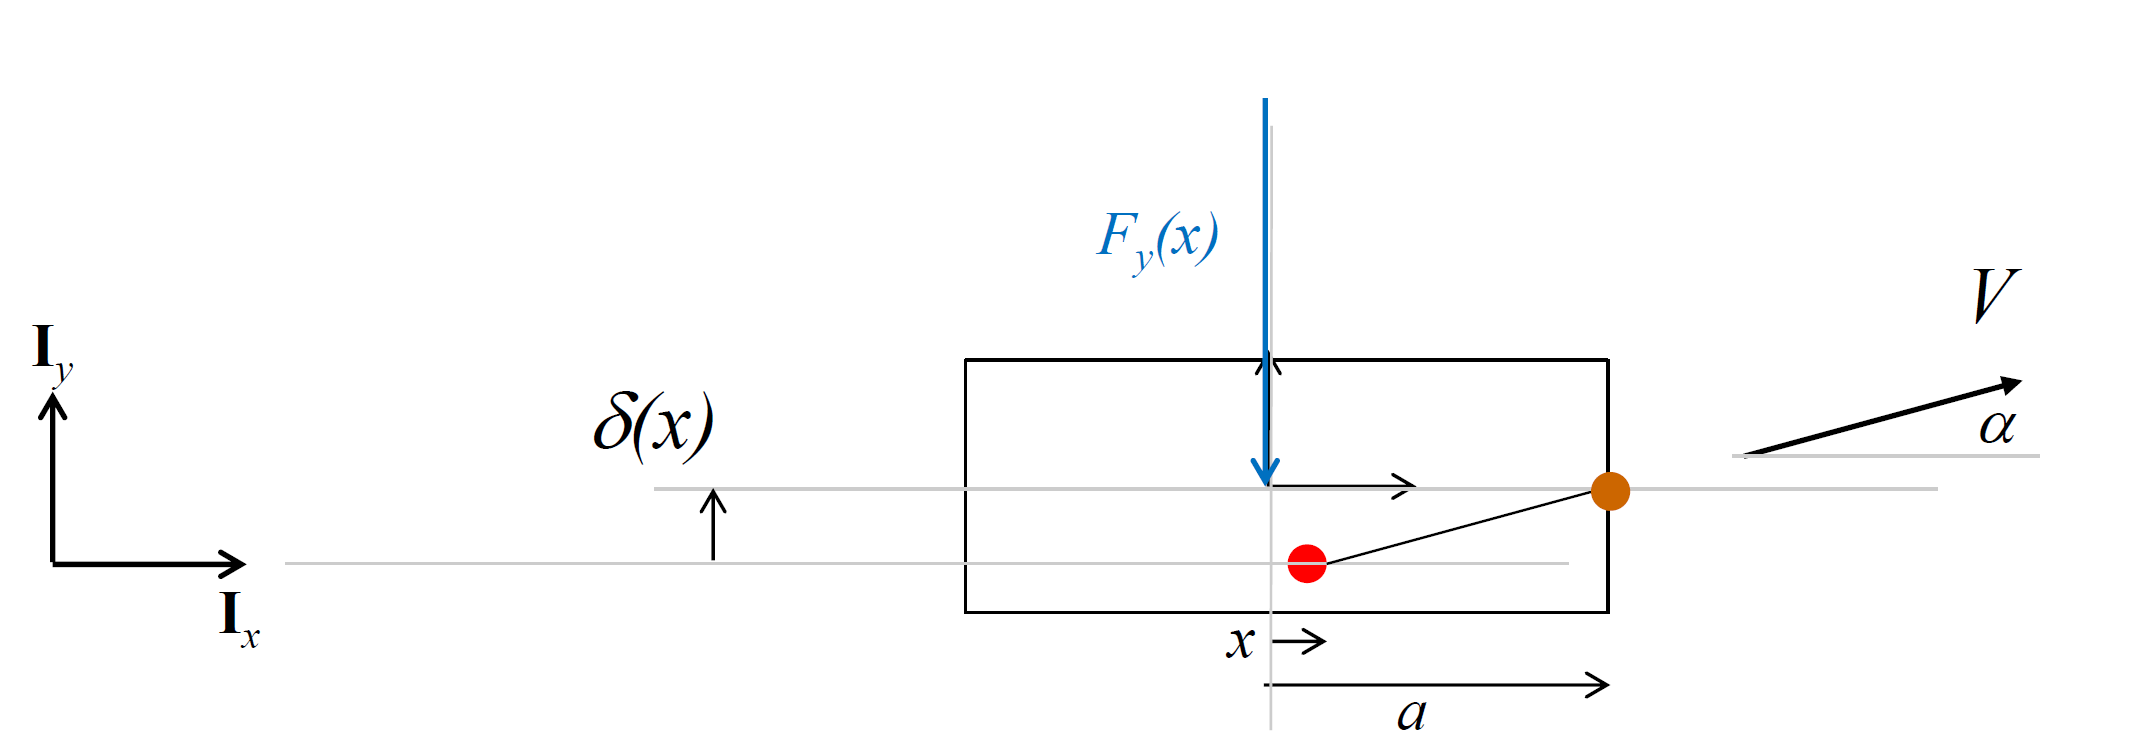
\includegraphics[width = 0.6\textwidth]{Couple_auto_stab.png}
\end{figure}

\vspace{-0.5cm}
\begin{equation*}
    \Delta F_y(x) = -C_y \delta(x) \Delta x = - C_y (a-x) tan(\alpha) \Delta x
\end{equation*}

La pression\footnote{$p(x)$ n'a pas vraiment les unités d'une pression comme en atteste la formule mais plutôt de [N/m]} est considérée comme distribuée paraboliquement selon l'axe longitudinal:
$$ p(x) = \cfrac{3 F_z}{4a}(1 - \cfrac{x^2}{a^2})$$

Donc d'après la loi de Coulomb, la force résultante ne peut pas dépasser :
$$\Delta F_{frot} \leq \mu \cdot | p(x) \Delta x | $$

Par ailleurs, comme on analyse un mouvement de braquage simple, la seul composante de la force de frottement est la force latéral ($\Delta F_{frot} = \Delta F_{y}(x)$). La condition de Coulomb donne donc lieu à :

\begin{figure}[H]
    \centering
    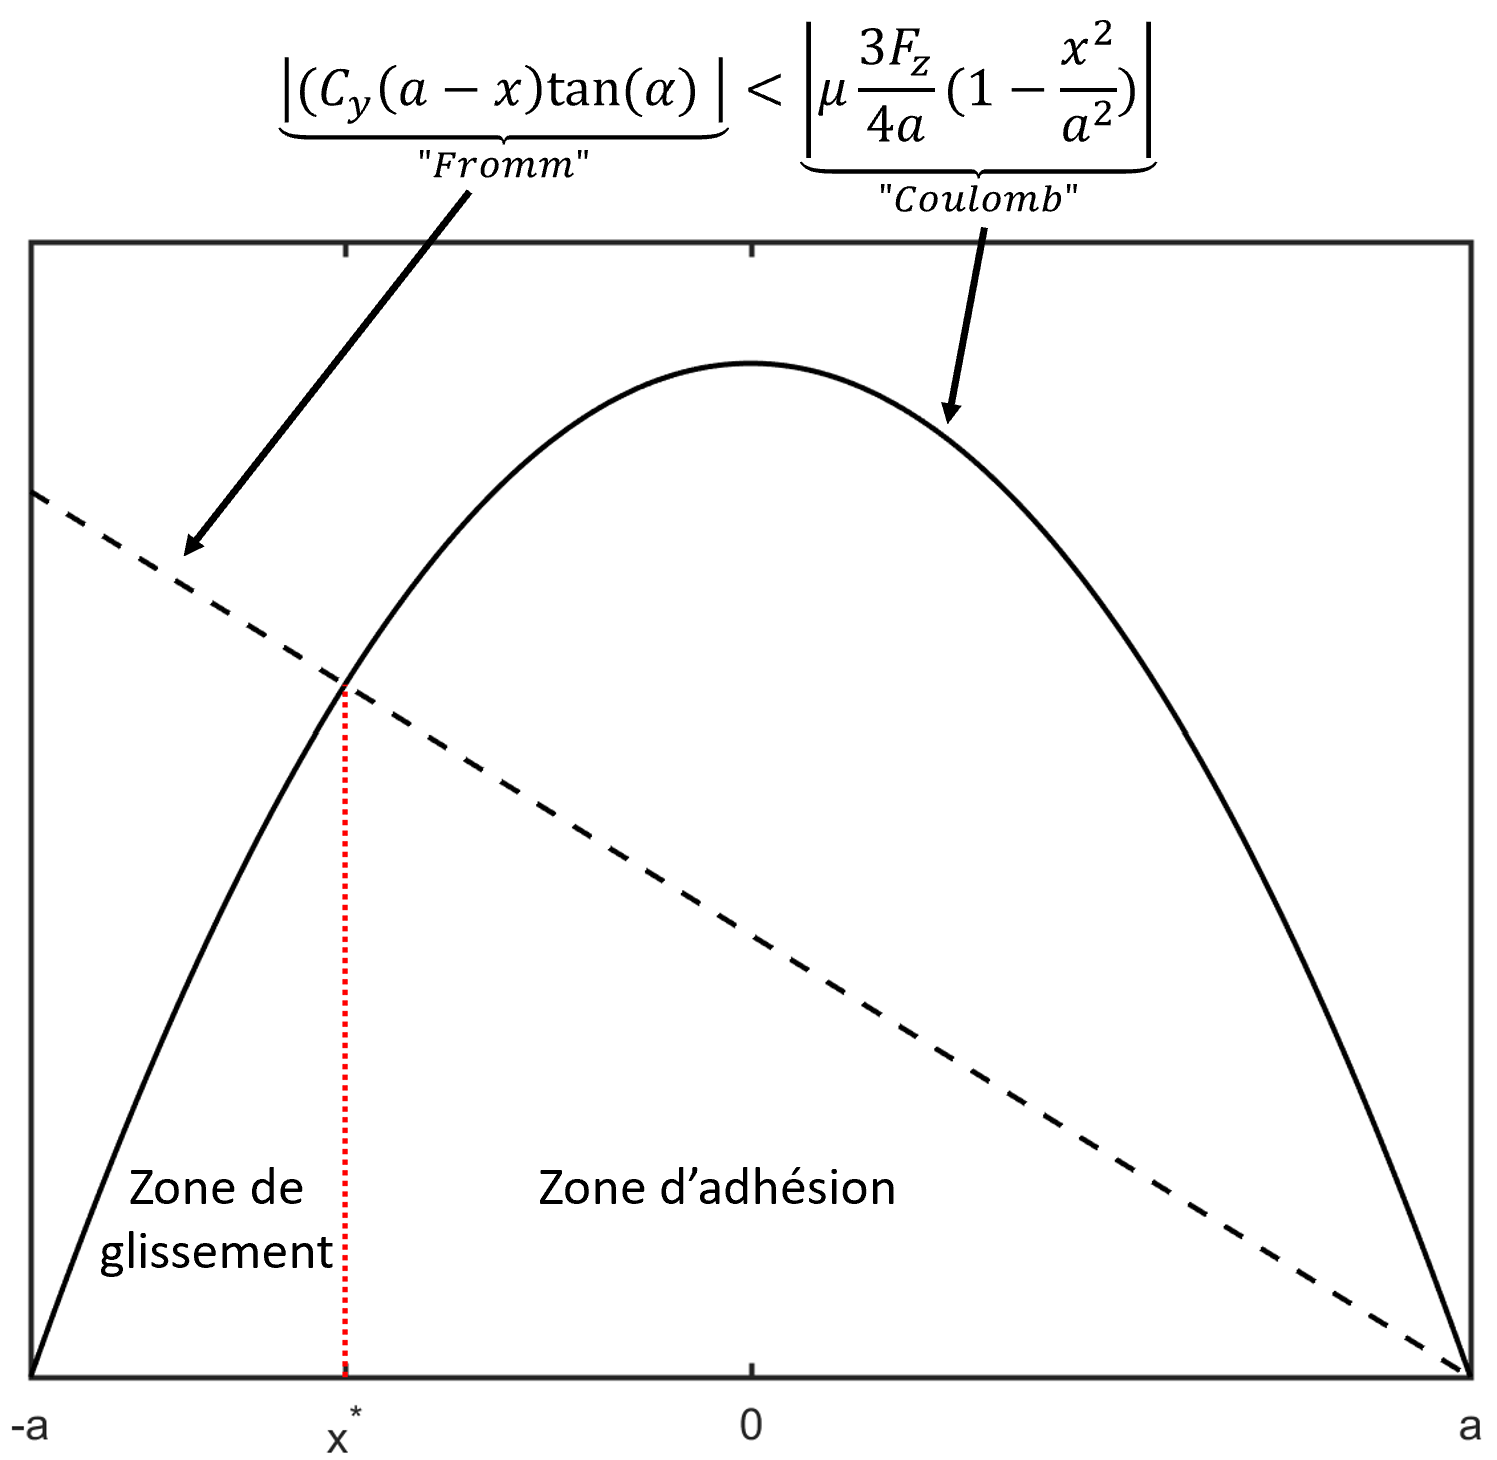
\includegraphics[width = 0.5\textwidth]{F_y.png}
\end{figure}

En calculant le point de transition $x^*$ ("Fromm" = "Coulomb"), il est possible de déterminer l'angle de glissement maximum ! C'est-à-dire l'angle $\alpha$ à partir duquel le pneu est en glissement pure.

Par ailleurs, la force latéral total est calculé en intégrant la relation de Fromm sur la zone d'adhérence et la relation de Coulomb sur la zone de glissement et en sommant les 2 :

\begin{equation*}
    F_y = - \int_{-a}^{x^*} \frac{3\mu F_z}{4a}\left(1-(\frac{x}{a})^2\right)dx - \int_{x^*}^{a} C_y(a-x)\tan{(\alpha)}dx
\end{equation*}

Le couple total lui est obtenu de la même manière (intégration sur les 2 zones) mais en multipliant $\Delta F_{y,Fromm}$ et $\Delta F_{y,Coulomb}$ par le bras de levier c'est-à-dire la distance à l'origine ou encore $x$ :

\begin{equation*}
    M_z = - \int_{-a}^{x^*} \frac{3\mu F_z}{4a}\left(1-(\frac{x}{a})^2\right) \cdot x \text{ }dx - \int_{x^*}^{a} C_y(a-x)\tan{(\alpha)} \cdot x \text{ }dx
\end{equation*}

Remarquons alors que ce couple est toujours positif ou nul. En effet, vu que la limite de Coulomb est symétrique par rapport à 0 :
\begin{itemize}
    \item Soit on est en total adhérence ($\alpha = 0 \Rightarrow$ ligne droite). Dès lors, résultante des forces latérales nul $\Rightarrow M_z = 0$
    \item Soit limiter par Fromm qui est d'autant plus restrictif que l'on se trouve proche du début de la zone de contact donc à droite de 0. Donc, la résultante de force du côté gauche de la zone de contact sera toujours plus grand la résultante du côté droit $\Rightarrow M_z > 0$
\end{itemize}

Ce couple va donc dans tous les cas tendre à réduire l'angle de glissement à 0 (c.à.d aligner la roue avec le vecteur vitesse). D'où son nom de couple auto-stabilisant.

\textbf{ATTENTION :} Il faut bien remarquer que le modèle de Fromm n'est qu'un modèle simplifié. En effet, en réalité, le couple auto-stabilisant peut devenir négatif lorsque le glissement devient trop important. On appelle se phénomène le "fusible mécanique" car il permet d'avertir le conducteur avisé que son véhicule se rapprochant dangereusement de la limite glissement (passage à full glissement). 

\paragraph{Glissement longitudinal simple :} pas d'angle (variation) de drift, pas de carrossage. Le glissement longitudinal provoque une force longitudinale. Dans le graphe ci-dessous, on remarque que pour de faibles angles de drift (angle de glissement), il y a un pic de force longitudinale pour un faible glissement. C'est ce pic qui est exploité par l'ABS !
\begin{figure}[H]
    \centering
    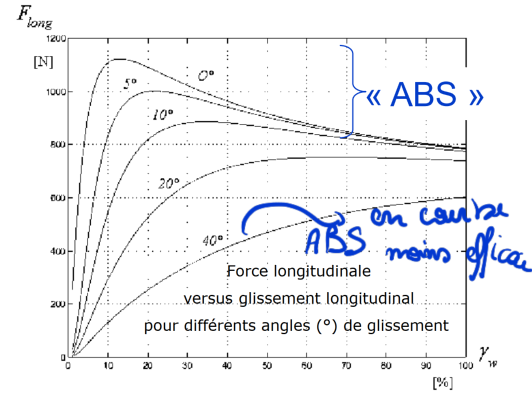
\includegraphics[width = 0.4\textwidth]{pure_longitudinal.PNG}
\end{figure}

\paragraph{Carrossage simple :} pas d'accélération/freinage, pas d'angle de drift. L'angle de carrossage provoque, à cause de la forme de cône du pneu sur le sol et de sa déflection (déformation), une force latérale et un couple d'alignement.

\subsection{Modèles de contact pneu-sol :}
\paragraph{Modèle "exaustif" :}
Permet de mixer les différents phénomènes décris ci-dessus. Notons que la force résultante est limitée par coulomb !
$$\sqrt{F_x^2 + F_y^2} < \mu \cdot |F_z| $$
Il s'agit d'un modèle paramétrique dérivé de celui de Fromm-Fiala.
Il est utile dans les cas où peu de données sont disponibles (bus, camion, Kiffy, ...) car il se base sur seulement 10 paramètres :
\begin{figure}[H]
    \begin{minipage}[b]{0.4\linewidth}
    \centering
        \begin{itemize}
            \item géométrie du pneu ($R_1$, $R_2$)
            \item résistance au roulement ($f_R$) 
            \item raideur et amortissement radial ($k_Z$,$c_Z$)
            \item coefficients de frottement ($f_s$,$f_d$)
            \item coefficients de raideur $C_\alpha$, $C_S$ et $C_\gamma$
        \end{itemize}
    \end{minipage}\hfill
    \begin{minipage}[b]{0.55\linewidth}
    \centering
        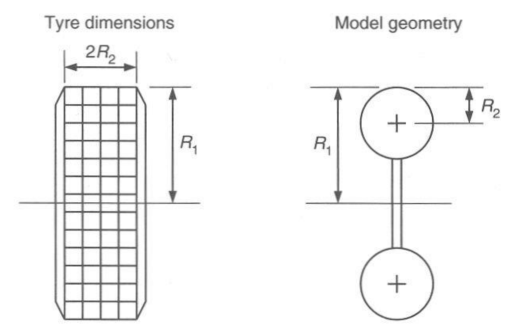
\includegraphics[width=0.8\linewidth]{modele_pneu.png}
    \end{minipage}
\end{figure}
\paragraph{Modèle semi-empirique :}
Basé sur la "formule magique" de Bakker-Pacejka. 
\textbf{Modèle basés sur des tests et donc valable pour un pneu particulier!}
Il y a plus de 100 coefficients à déterminer par mesure.

\paragraph{Modèles plus avancés :}
D'autres modèles sont possibles :
\begin{itemize}
    \item Basé sur la souplesses (raideur) de mouvement du pneu sur sa jante.
    \item Modèle de "corde(s)" qui se déforme(nt).
    \item Modèle d'éléments finis.
\end{itemize}

\subsection{Comportement en virage :}
\paragraph{Modèle "vélo" :}
On aplatit la voiture pour considérer le comportement moyen par essieux. Pour cela on commence par déterminer l'angle de braquage moyen (angle de Ackermann) :

\begin{equation*}
    \cot{\delta} = \frac{\cot{\delta_{int}} + \cot{\delta_{ext}}}{2}
\end{equation*}

Qui sous l'hypothèse de petits angles, donne :

\begin{equation*}
    \delta = \frac{L}{R}
\end{equation*}

Dans laquelle, $L$ est l'empattement, $R$ est le rayon de courbure. Sachant que les angles de braquage de la roue intérieure et extérieure sont respectivement (fonction de la voie $v$):
\begin{align*}
    \delta_{int} &= \cfrac{L}{(R-v/2)} \\
    \delta_{ext} &= \cfrac{L}{(R+v/2)}
\end{align*}
\begin{figure}[H]
    \centering
    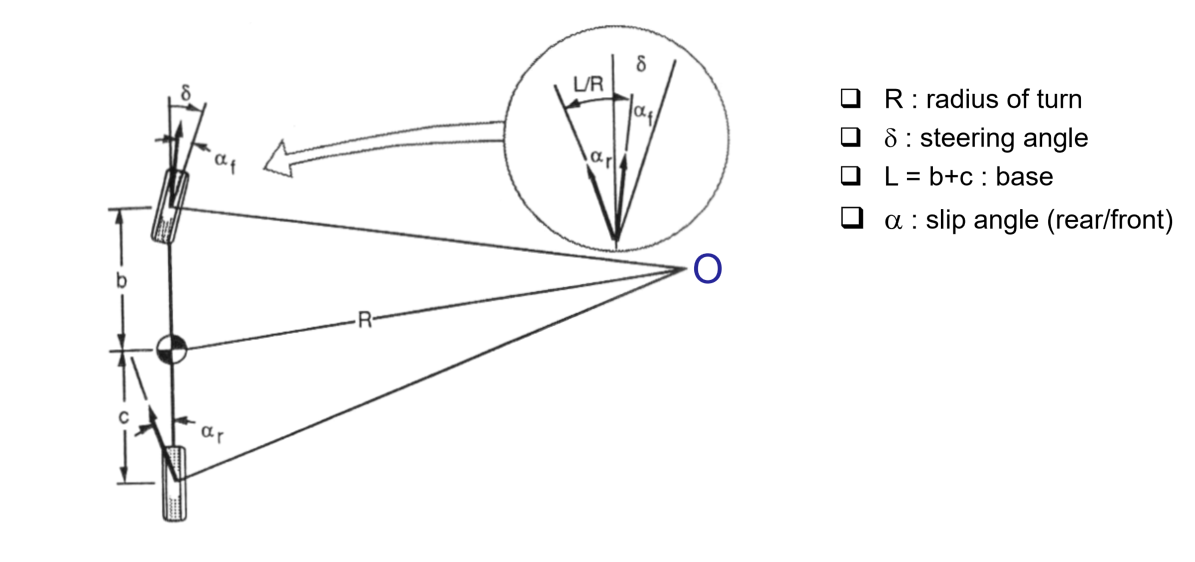
\includegraphics[width=0.8\textwidth]{velo.PNG}
    \caption{Voiture "aplatie".}
    \label{velo}
\end{figure}
En virage (voir schéma angles \autoref{velo}):
\begin{equation}
\label{braquage_velo}
    \text{Angle volant :   } \delta = 57,3 L/R + \alpha_f + \alpha_r 
\end{equation} 
Le tout en degré ($57,3 = $ degrés par radian)!
L'angle du volant doit être d'autant plus grand que l'on glisse de l'avant, et d'autant plus petit que l'on glisse de l'arrière. 
En utilisant Newton et Euler, supposant que $F_y = C_\alpha \cdot \alpha$ et en définissant le poids sur l'avant $W_f$ (idem pour l'arrière) tel que:
$$m \cdot \cfrac{c}{L} = \cfrac{M_G}{g} \cdot \cfrac{c}{L} = \cfrac{W_f}{g} $$
On détermine les angles de drift (glissement):
\begin{align*}
    \alpha_f &= \cfrac{W_f V^2}{C_{\alpha f} g R}\\
    \alpha_r &= \cfrac{W_r V^2}{C_{\alpha r} g R}
\end{align*}
Ce qui permet de réécrire \autoref{braquage_velo} :
\begin{equation}
\label{braquage_velo2}
    \delta = 57,3 L/R + \Big ( \cfrac{W_f}{C_{\alpha f}} - \cfrac{W_r}{C_{\alpha r}}\Big ) \cdot \cfrac{V^2}{g R} = 57,3 L/R + K \cdot \alpha_y
\end{equation} 
$K = \Big ( \cfrac{W_f}{C_{\alpha f}} - \cfrac{W_r}{C_{\alpha r}}\Big )$ est le gradient de sous-virage. La voiture est:
\begin{itemize}
    \item \textbf{$K$ positif : }Sous-vireuse
    \item \textbf{$K$ négatif : }Sur-vireuse
\end{itemize}
Remarquons que si la voiture est sur-vireuse, il existera une vitesse critique à laquelle $\delta=0$ et où la voiture tournera toute seule sans braquage... !

\section{MBS Routier :}
Géométriquement, la roue (+ le pneu) est un disque sans épaisseur de rayon variable $r_W$. Celle-ci a un point de contact $\mathbf{Q}$ avec le sol dont le profil est une fonction de la position $(x,y)$ :
$$ z = \mu(x,y)$$
Les forces et couples de contact s'appliquent en ce point $\mathbf{Q}$. Le point de contact sur le sol est nommé $\mathbf{P}$. Comme pour le contact roue/rail, on considère un repère géométrique $\mathbf{\hat{X}}$ (qui ne tourne pas) et un repère attaché à la roue $\mathbf{\hat{Y}}$. Le repère $\mathbf{\hat{T}}$ est le repère tangent au niveau du point de contact.
\begin{figure}[H]
    \centering
    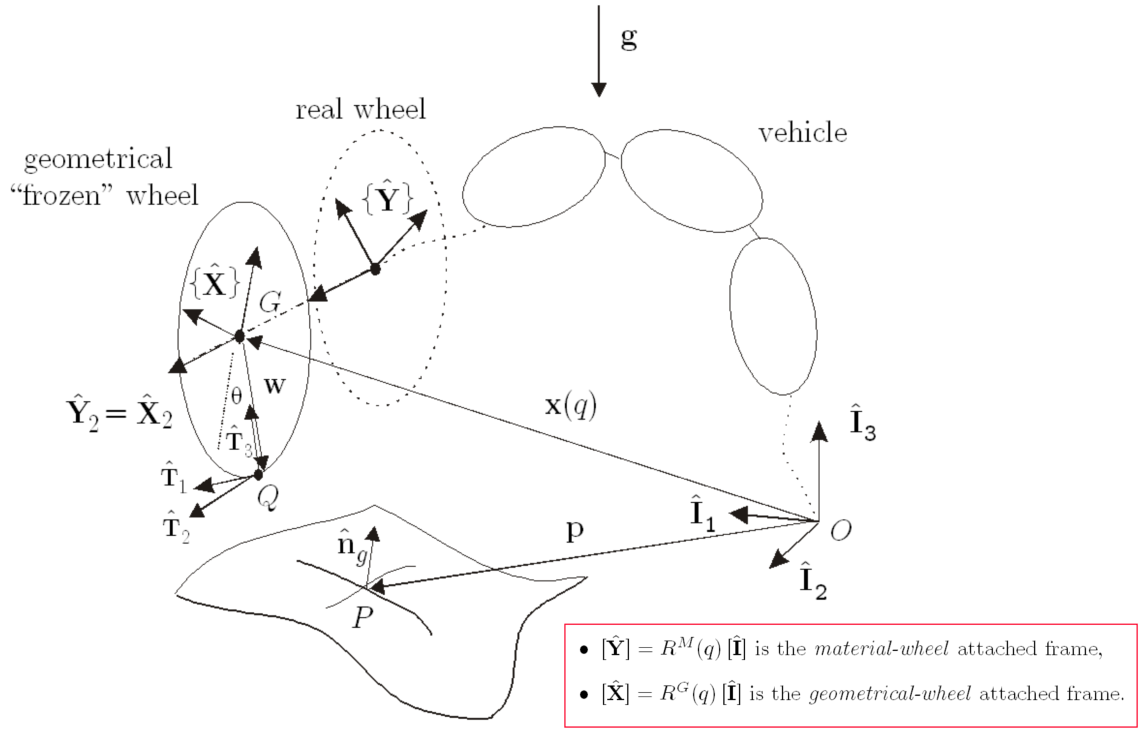
\includegraphics[width=0.8\textwidth]{roue.PNG}
    \caption{Représentation de la roue. Attention $\theta$ n'y est pas la rotation de la roue mais une variable auxiliaire qui peut être non nul lorsque le profil n'est pas plan.}
    \label{roue}
\end{figure}
Deux variables auxiliaires permettent de localiser le point de contact : l'angle entre le repère géométrique (fixe) et le point de contact $\theta$ (qui est non nul lorsque le profil du sol n'est pas plan) et le rayon de la roue $r_w$.
Si il y a contact, alors $r_w \leq r_{nom}$ car le pneu peut s'écraser ($r_{nom}$ étant le rayon de la roue non chargée). Notons que si le contact se perd $r_w > r_{nom}$.
Deux contraintes s'appliquent sur ces variables auxiliaires (on parle alors de \textbf{pseudo-contrainte} !!!):
\begin{align*}
    h_1^w(q,r_w,\theta) &= z - \mu(x,y) = 0\\
    h_2^w(q,r_w, \theta) &= \mathbf{\hat{T}}_1 \cdot \mathbf{\hat{n}}_g = 0
\end{align*}
La première impose que la roue touche le sol et la seconde impose que la roue "géométrique" soit tangente au sol ($\mathbf{\hat{T}}_1 $ perpendiculaire à la normale au sol $\mathbf{\hat{n}}_g$). Il est également nécessaire de vérifier que le centre de la roue est bien au-dessus du sol:
$$r_w > 0 $$
Pour calculer les forces les définitions des angles de carrossage $\phi_w$ et de drift $\alpha_w$ sont nécessaire :
\begin{figure}[H]
    \begin{minipage}[b]{0.45\linewidth}
    \centering
        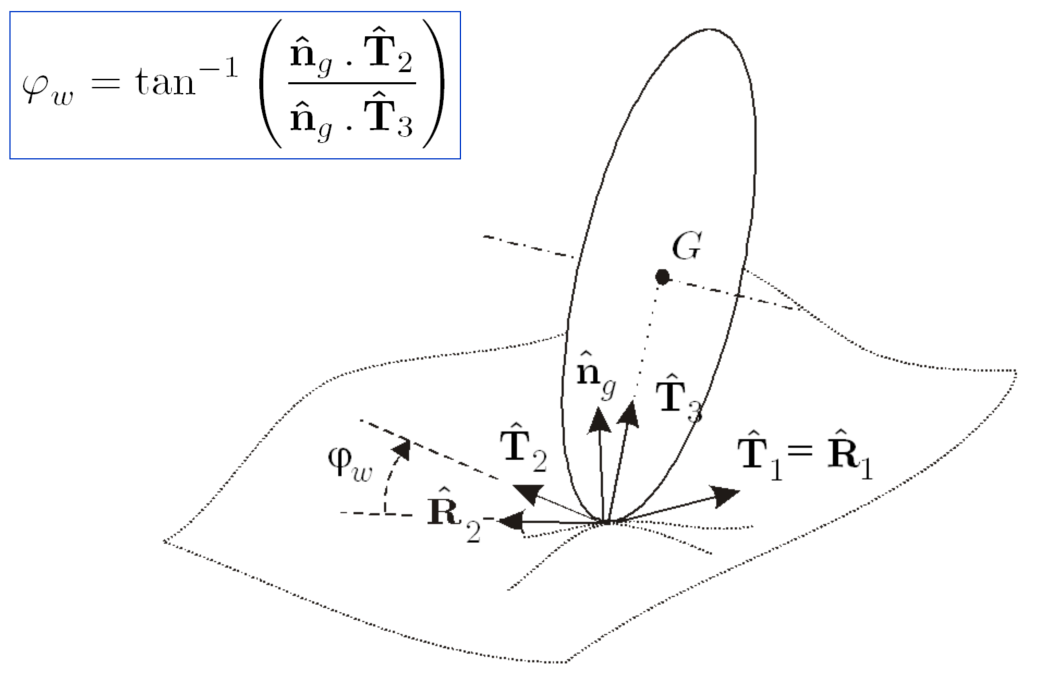
\includegraphics[width=0.8\linewidth]{carrossage.PNG}
        \caption{Angle de carrossage.}
    \end{minipage}\hfill
    \begin{minipage}[b]{0.45\linewidth}
    \centering
        \includegraphics[width=0.8\linewidth]{drift.PNG}
        \caption{Angle de drift (glissement) ou de dérive.}
    \end{minipage}
\end{figure}
La pénétration du pneu dans le sol est une fonction de l'angle de carrossage $\phi_w$:
$$p_w = max\{0, cos(\phi_w) \cdot (r_{nom}-r_w) \} $$
Les forces et couples à calculer sont représenter dans la \autoref{forces_roue}.
\begin{figure}[H]
    \centering
    \includegraphics[width = 0.6\textwidth]{forces_roue.PNG}
    \caption{Forces et couples à calculer. $M_{roll}$ est "l'overturning", $M_{pitch}$ est la résistance à la rotation de la roue et $M_{yaw}$ est le couple d'alignement.}
    \label{forces_roue}
\end{figure}

\paragraph{Modèle de force verticale :}
Un modèle populaire est de calculer la force verticale par un ressort-amortisseur fonction de la pénétration $p_w$ et de sa vitesse $\dot{p}_w$:
$$F_{vert} = K_{rad} p_w + D_{rad} \dot{p}_w $$

\paragraph{Modèle de Calspan :}
Le modèle de Calspan (voir \autoref{Calspan}) se limite au calcul de la force latérale $F_{lat}$ et du couple d'alignement $M_{yaw}$ : 
\begin{align*}
    F_{lat} &= f F_{vert} g(\overline{\alpha}) F_{slip} \\
    M_{yaw} &= (F_1 F_{vert} + F_2 |F_{lat}|) F_{lat}
\end{align*}
Sur base d'un coefficient de frottement latéral $f=(B_1 F_{vert} + B_2 + B_3(F_{vert})^2 ) S_N$, d'une fonction de forme (des forces latérales) $g(\overline{\alpha})$ où $\overline{\alpha}$ est un angle de glissement adimensionnel équivalent et de différents coefficients tabulés.

\paragraph{Modèle de Bakker :}
Modèle qui calcule dans un premier temps les forces longitudinales, latérales et le couple d'alignement de manière indépendante les unes des autres, puis en appliquant un coefficient dans le cas où le véhicule a un mouvement de glissement latéralet longitudinal en même temps. Côté un peu "formule magique" ... !

\section{Dynamique des deux roues : }

Les deux roues sont intéressants du fait de la non-linéarité de leur dynamique et de leur contrôle (Notamment la stabilité à haute vitesse mais pas à l'arrêt).
\paragraph{Modèle énergétique :}
Basé sur les énergies due aux inerties de rotation.
$$\tau_1^2 \ddot{\theta} - \theta = -K(\tau_2 \dot{\delta_f} + \delta_f + \tau_3 \dot{\delta_r} - \delta_r $$
Où $\theta$ est l'angle de roulis du vélo (inclinaison par rapport à la verticale), $\delta_f$ est l'angle entre le guidon et le châssis, $\delta_r $ et l'angle entre l'axe de la roue arrière et le châssis (généralement nul). Ce modèle peut être vu comme une fonction de tranfert entre l'angle du guidon et l'inclinaison du vélo :
\begin{figure}[H]
    \centering
    \includegraphics[width=0.6\textwidth]{transfert_velo.PNG}
\end{figure}
On remarque déjà malgré la simplicité du modèle que pour effectuer un virage (incliner le vélo d'un côté) il est nécessaire de contre-braquer d'abord.
 
\paragraph{Modèle Whipple :}
Equations simplifiées mais non linéaires , 4 corps $\Rightarrow$ 3 ddl, 25 paramètres. 

\paragraph{Modèle multi-corps :}
Permet plus de tests différents !

\paragraph{Analyse modale :}
Si on considère du roulement sans glissement un vélo à uniquement 3 ddl, et si on ne se préocupe pas des modes liés à l'avance (que l'on considère comme driven) on a donc $2\cdot 2$ modes propres :
\begin{itemize}
    \item 2 modes de louvoiement (le vélo fait des slaloms)
    \item un mode de renversement (faire des roues arrière par exemple)
    \item un mode de guidonnage (le guidon vibre et tourne tout seul $\Rightarrow$ aller voir "Guidonnage moto" sur Youtube, vous ne serez pas déçu !) 
    
\end{itemize}
\begin{figure}[H]
    \centering
    \includegraphics[width=0.7\textwidth]{velo_modal.PNG}
    \caption{Analyse modale d'un vélo}
    \label{velo_modal}
\end{figure}


\end{document}
